% !TeX spellcheck = pl_PL
%%%%%%%%%%%%%%%%%%%%%%%%%%%%%%%%%%%%%%%%%%%
%                                        %
% Szablon pracy dyplomowej magisterskiej %
% zgodny  z aktualnymi  przepisami  SZJK %
%                                        %
%%%%%%%%%%%%%%%%%%%%%%%%%%%%%%%%%%%%%%%%%%
%                                        %
%  (c) Krzysztof Simiński, 2018-2023     %
%                                        %
%%%%%%%%%%%%%%%%%%%%%%%%%%%%%%%%%%%%%%%%%%
%                                        %
% Najnowsza wersja szablonów jest        %
% podstępna pod adresem                  %
% github.com/ksiminski/polsl-aei-theses  %
%                                        %
%%%%%%%%%%%%%%%%%%%%%%%%%%%%%%%%%%%%%%%%%%
%
%
% Projekt LaTeXowy zapewnia odpowiednie formatowanie pracy,
% zgodnie z wymaganiami Systemu zapewniania jakości kształcenia.
% Proszę nie zmieniać ustawień formatowania (np. fontu,
% marginesów, wytłuszczeń, kursywy itd. ).
%
% Projekt można kompilować na kilka sposobów.
%
% 1. kompilacja pdfLaTeX
%
% pdflatex main
% bibtex   main
% pdflatex main
% pdflatex main
%
%
% 2. kompilacja XeLaTeX
%
% Kompilatacja przy użyciu XeLaTeXa różni się tym, że na stronie
% tytułowej używany jest font Calibri. Wymaga to jego uprzedniego
% zainstalowania.
%
% xelatex main
% bibtex  main
% xelatex main
% xelatex main
%
%
%%%%%%%%%%%%%%%%%%%%%%%%%%%%%%%%%%%%%%%%%%%%%%%%%%%%%
% W przypadku pytań, uwag, proszę pisać na adres:   %
%      krzysztof.siminski(małpa)polsl.pl            %
%%%%%%%%%%%%%%%%%%%%%%%%%%%%%%%%%%%%%%%%%%%%%%%%%%%%%
%
% Chcemy ulepszać szablony LaTeXowe prac dyplomowych.
% Wypełniając ankietę spod poniższego adresu pomogą
% Państwo nam to zrobić. Ankieta jest całkowicie
% anonimowa. Dziękujemy!


% https://docs.google.com/forms/d/e/1FAIpQLScyllVxNKzKFHfILDfdbwC-jvT8YL0RSTFs-s27UGw9CKn-fQ/viewform?usp=sf_link
%
%%%%%%%%%%%%%%%%%%%%%%%%%%%%%%%%%%%%%%%%%%%%%%%%%%%%%%%%%%%%%%%%%%%%%%%%%

%%%%%%%%%%%%%%%%%%%%%%%%%%%%%%%%%%%%%%%%%%%%%%%
%                                             %
% PERSONALIZACJA PRACY – DANE PRACY           %
%                                             %
%%%%%%%%%%%%%%%%%%%%%%%%%%%%%%%%%%%%%%%%%%%%%%%

% Proszę wpisać swoje dane w poniższych definicjach.

% TODO
% dane autora
\newcommand{\FirstNameAuthor}{Imię}
\newcommand{\SurnameAuthor}{Nazwisko}
\newcommand{\IdAuthor}{$\langle$wpisać właściwy$\rangle$}   % numer albumu  (bez $\langle$ i $\rangle$)

% drugi autor:
%\newcommand{\FirstNameCoauthor}{Imię}   % Jeżeli jest drugi autor, to tutaj należy podać imię.
%\newcommand{\SurnameCoauthor}{Nazwisko} % Jeżeli jest drugi autor, to tutaj należy podać nazwisko.
%\newcommand{\IdCoauthor}{$\langle$wpisać właściwy$\rangle$}  % numer albumu drugiego autora (bez $\langle$ i $\rangle$)
% Gdy nie ma drugiego autora, należy zostawić poniższe definicje puste, jak poniżej. Gdy jest drugi autor, należy zakomentować te linie.
\newcommand{\FirstNameCoauthor}{} % Jeżeli praca ma tylko jednego autora, to dane drugiego autora zostają puste.
\newcommand{\SurnameCoauthor}{}   % Jeżeli praca ma tylko jednego autora, to dane drugiego autora zostają puste.
\newcommand{\IdCoauthor}{}  % Jeżeli praca ma tylko jednego autora, to dane drugiego autora zostają puste.
%%%%%%%%%%

\newcommand{\Supervisor}{$\langle$tytuł lub stopień naukowy oraz imię i nazwisko$\rangle$}     % dane promotora (bez $\langle$ i $\rangle$)
\newcommand{\Title}{Tytuł pracy dyplomowej magisterskiej}           % tytuł pracy po polsku
\newcommand{\TitleAlt}{Thesis title in English}                     % thesis title in English
\newcommand{\Program}{$\langle$wpisać właściwy$\rangle$}            % kierunek studiów  (bez $\langle$ i $\rangle$)
\newcommand{\Specialisation}{$\langle$wpisać właściwą$\rangle$}     % specjalność  (bez $\langle$ i $\rangle$)
\newcommand{\Departament}{$\langle$wpisać właściwą$\rangle$}        % katedra promotora  (bez $\langle$ i $\rangle$)

% Jeżeli został wyznaczony promotor pomocniczy lub opiekun, proszę go/ją wpisać ...
\newcommand{\Consultant}{$\langle$stopień naukowy imię i nazwisko$\rangle$} % dane promotora pomocniczego, opiekuna (bez $\langle$ i $\rangle$)
% ... w przeciwnym razie proszę zostawić puste miejsce jak poniżej:
%\newcommand{\Consultant}{} % brak promotowa pomocniczego / opiekuna

% koniec fragmentu do modyfikacji
%%%%%%%%%%%%%%%%%%%%%%%%%%%%%%%%%%%%%%%%%%


%%%%%%%%%%%%%%%%%%%%%%%%%%%%%%%%%%%%%%%%%%%%%%%
%                                             %
% KONIEC PERSONALIZACJI PRACY                 %
%                                             %
%%%%%%%%%%%%%%%%%%%%%%%%%%%%%%%%%%%%%%%%%%%%%%%

%%%%%%%%%%%%%%%%%%%%%%%%%%%%%%%%%%%%%%%%


%%%%%%%%%%%%%%%%%%%%%%%%%%%%%%%%%%%%%%%%%%%%%%%
%                                             %
% PROSZĘ NIE MODYFIKOWAĆ PONIŻSZYCH USTAWIEŃ! %
%                                             %
%%%%%%%%%%%%%%%%%%%%%%%%%%%%%%%%%%%%%%%%%%%%%%%



\documentclass[a4paper,twoside,12pt]{book}
\usepackage[utf8]{inputenc}                                      
\usepackage[T1]{fontenc}  
\usepackage{amsmath,amsfonts,amssymb,amsthm}


\usepackage[british,polish]{babel} 
\usepackage{indentfirst}
\usepackage{xurl}
\usepackage{xstring}
\usepackage{ifthen}



\usepackage{ifxetex}

\ifxetex
	\usepackage{fontspec}
	\defaultfontfeatures{Mapping=tex—text} % to support TeX conventions like ``——-''
	\usepackage{xunicode} % Unicode support for LaTeX character names (accents, European chars, etc)
	\usepackage{xltxtra} % Extra customizations for XeLaTeX
\else
	\usepackage{lmodern}
\fi



\usepackage[margin=2.5cm]{geometry}
\usepackage{graphicx} 
\usepackage{hyperref}
\usepackage{booktabs}
\usepackage{tikz}
\usepackage{pgfplots}
\usepackage{mathtools}
\usepackage{geometry}
\usepackage{subcaption}   % subfigures
\usepackage[page]{appendix} % toc,
\renewcommand{\appendixtocname}{Dodatki}
\renewcommand{\appendixpagename}{Dodatki}
\renewcommand{\appendixname}{Dodatek}

\usepackage{csquotes}
\usepackage[natbib=true,backend=bibtex,maxbibnames=99]{biblatex}  % kompilacja bibliografii BibTeXem
%\usepackage[natbib=true,backend=biber,maxbibnames=99]{biblatex}  % kompilacja bibliografii Biberem
\bibliography{biblio}

\usepackage{ifmtarg}   % empty commands  

\usepackage{setspace}
\onehalfspacing


\frenchspacing

%%%%%%%%%%%%%%%%%%%%%%%%%%%%%%%%%%
% środowiska dla definicji, twierdzenia, przykładu
\usepackage{amsthm}

\newtheorem{Definition}{Definicja}
\newtheorem{Example}{Przykład}
\newtheorem{Theorem}{Twierdzenie}
%%%%%%%%%%%%%%%%%%%%%%%%%%%%%%%%%%

%%%% TODO LIST GENERATOR %%%%%%%%%

\usepackage{color}
\definecolor{brickred}      {cmyk}{0   , 0.89, 0.94, 0.28}

\makeatletter \newcommand \kslistofremarks{\section*{Uwagi} \@starttoc{rks}}
  \newcommand\l@uwagas[2]
    {\par\noindent \textbf{#2:} %\parbox{10cm}
{#1}\par} \makeatother


\newcommand{\ksremark}[1]{%
{%\marginpar{\textdbend}
{\color{brickred}{[#1]}}}%
\addcontentsline{rks}{uwagas}{\protect{#1}}%
}

\newcommand{\comma}{\ksremark{przecinek}}
\newcommand{\nocomma}{\ksremark{bez przecinka}}
\newcommand{\styl}{\ksremark{styl}}
\newcommand{\ortografia}{\ksremark{ortografia}}
\newcommand{\fleksja}{\ksremark{fleksja}}
\newcommand{\pauza}{\ksremark{pauza `--', nie dywiz `-'}}
\newcommand{\kolokwializm}{\ksremark{kolokwializm}}
\newcommand{\cudzyslowy}{\ksremark{,,polskie cudzysłowy''}}

%%%%%%%%%%%%%% END OF TODO LIST GENERATOR %%%%%%%%%%%

\newcommand{\printCoauthor}{%		
    \StrLen{\FirstNameCoauthor}[\FNCoALen]
    \ifthenelse{\FNCoALen > 0}%
    {%
		{\large\bfseries\Coauthor\par}
	
		{\normalsize\bfseries \LeftId: \IdCoauthor\par}
    }%
    {}
} 

%%%%%%%%%%%%%%%%%%%%%
\newcommand{\autor}{%		
    \StrLen{\FirstNameCoauthor}[\FNCoALenXX]
    \ifthenelse{\FNCoALenXX > 0}%
    {\FirstNameAuthor\ \SurnameAuthor, \FirstNameCoauthor\ \SurnameCoauthor}%
	{\FirstNameAuthor\ \SurnameAuthor}%
}
%%%%%%%%%%%%%%%%%%%%%

\StrLen{\FirstNameCoauthor}[\FNCoALen]
\ifthenelse{\FNCoALen > 0}%
{%
\author{\FirstNameAuthor\ \SurnameAuthor, \FirstNameCoauthor\ \SurnameCoauthor}
}%
{%
\author{\FirstNameAuthor\ \SurnameAuthor}
}%

%%%%%%%%%%%% ZYWA PAGINA %%%%%%%%%%%%%%%
% brak kapitalizacji zywej paginy
\usepackage{fancyhdr}
\pagestyle{fancy}
\fancyhf{}
\fancyhead[LO]{\nouppercase{\it\rightmark}}
\fancyhead[RE]{\nouppercase{\it\leftmark}}
\fancyhead[LE,RO]{\it\thepage}


\fancypagestyle{tylkoNumeryStron}{%
   \fancyhf{} 
   \fancyhead[LE,RO]{\it\thepage}
}

\fancypagestyle{bezNumeracji}{%
   \fancyhf{} 
   \fancyhead[LE,RO]{}
}


\fancypagestyle{NumeryStronNazwyRozdzialow}{%
   \fancyhf{} 
   \fancyhead[LE]{\nouppercase{\autor}}
   \fancyhead[RO]{\nouppercase{\leftmark}} 
   \fancyfoot[CE, CO]{\thepage}
}


%%%%%%%%%%%%% OBCE WTRETY  
\newcommand{\obcy}[1]{\emph{#1}}
\newcommand{\english}[1]{{\selectlanguage{british}\obcy{#1}}}
%%%%%%%%%%%%%%%%%%%%%%%%%%%%%

% polskie oznaczenia funkcji matematycznych
\renewcommand{\tan}{\operatorname {tg}}
\renewcommand{\log}{\operatorname {lg}}

% jeszcze jakies drobiazgi

\newcounter{stronyPozaNumeracja}

%%%%%%%%%%%%%%%%%%%%%%%%%%% 
\newcommand{\printOpiekun}[1]{%		

    \StrLen{\Consultant}[\mystringlen]
    \ifthenelse{\mystringlen > 0}%
    {%
       {\large{\bfseries OPIEKUN, PROMOTOR POMOCNICZY}\par}
       
       {\large{\bfseries \Consultant}\par}
    }%
    {}
} 
%
%%%%%%%%%%%%%%%%%%%%%%%%%%%%%%%%%%%%%%%%%%%%%%
 
% Proszę nie modyfikować poniższych definicji!
\newcommand{\Author}{\FirstNameAuthor\ \MakeUppercase{\SurnameAuthor}} 
\newcommand{\Coauthor}{\FirstNameCoauthor\ \MakeUppercase{\SurnameCoauthor}}
\newcommand{\Type}{PRACA MAGISTERSKA}
\newcommand{\Faculty}{Wydział Automatyki, Elektroniki i Informatyki} 
\newcommand{\Polsl}{Politechnika Śląska}
\newcommand{\Logo}{politechnika_sl_logo_bw_pion_pl.pdf}
\newcommand{\LeftId}{Nr albumu}
\newcommand{\LeftProgram}{Kierunek}
\newcommand{\LeftSpecialisation}{Specjalność}
\newcommand{\LeftSUPERVISOR}{PROWADZĄCY PRACĘ}
\newcommand{\LeftDEPARTMENT}{KATEDRA}
%%%%%%%%%%%%%%%%%%%%%%%%%%%%%%%%%%%%%%%%%%%%%%

%%%%%%%%%%%%%%%%%%%%%%%%%%%%%%%%%%%%%%%%%%%%%%%
%                                             %
% KONIEC USTAWIEŃ                             %
%                                             %
%%%%%%%%%%%%%%%%%%%%%%%%%%%%%%%%%%%%%%%%%%%%%%%




%%%%%%%%%%%%%%%%%%%%%%%%%%%%%%%%%%%%%%%%%%%%%%%
%                                             %
% MOJE PAKIETY, USTAWIENIA ITD                %
%                                             %
%%%%%%%%%%%%%%%%%%%%%%%%%%%%%%%%%%%%%%%%%%%%%%%

% Tutaj proszę umieszczać swoje pakiety, makra, ustawienia itd.



 

\newcommand{\model}[1]{\mathcal{#1}}
\newcommand{\modelU}{\model{U}}
\newcommand{\modelL}{\model{L}}

\newcommand{\modul}[1]{\left( #1 \right)}

\newcommand{\Upper}{`upper'}
\newcommand{\Lower}{`lower'}

\newcommand{\loss}{\mathcal{L}}

\newcommand{\dwielinie}[2]{\substack{#1\\#2}}
\newcommand{\kardynalnosc}{\kappa}
\newcommand{\specyficznosc}{\sigma}
\newcommand{\czystosc}{\zeta}

\DeclareMathOperator{\ksiIS}{\mathrm{is}}
\DeclareMathOperator{\ksiLIKE}{\mathrm{like}}
\DeclareMathOperator{\ksiAND}{\mathrm{and}}

\DeclareMathOperator{\ksiIF}{\mathrm{IF}}
\DeclareMathOperator{\ksiTHEN}{\mathrm{THEN}}


\newcommand{\rozniczka}[2]{\frac{\partial #1}{\partial #2}}  

\newcommand{\klaster}{c}
\newcommand{\srodek}{\macierz{v}}
\newcommand{\fpar}{f}   % fuzzification parameter
\newcommand{\waga}{\eta}  % example's weight
\newcommand{\odleglosc}{t}  % distance
\newcommand{\relacja}[1]{\boldsymbol{#1}} % relation

\newcommand{\kernel}{k}

\newcommand{\term}[1]{\mathfrak{#1}}
\newcommand{\zbior}[1]{\mathbb{#1}}  % set
\newcommand{\macierz}[1]{{\boldsymbol{\mathrm{#1}}}}  
\newcommand{\wektor}[1]{\macierz{\MakeLowercase{#1}}}
\newcommand{\newItem}[2]{%
  \expandafter\def\csname #1\endcsname {\MakeLowercase{#2}} %
  \expandafter\def\csname n#1\endcsname {\MakeUppercase{#2}} %
  \expandafter\def\csname z#1\endcsname {\zbior{\MakeUppercase{#2}}} %
  \expandafter\def\csname t#1\endcsname {\term{\MakeLowercase{#2}}} %
  \expandafter\def\csname m#1\endcsname {\macierz{\MakeUppercase{#2}}} %
  \expandafter\def\csname w#1\endcsname {\wektor{#2}} %
  }

%\newItem{Implikacja}{b'}
%\newItem{Membership}{\mu}
%\newItem{Membership}{\mu}
\newItem{estimators}{\theta}
\newItem{weight}{\omega}
\newItem{Atrybut}{a}
\newItem{Centre}{v}
\newItem{ClusterMembership}{\mu}
\newItem{Decyzja}{y}
\newItem{Deskryptor}{x}
\newItem{Distance}{d}
\newItem{Etykieta}{e}
\newItem{GlobalTypicality}{g}
\newItem{Granula}{g}
\newItem{Implikacja}{c}
\newItem{Individual}{q} 
\newItem{Iteracja}{i}
%\newItem{Klasa}{\delta}
\newItem{Zgoda}{z}
\newItem{Klasa}{c}
\newItem{Klasyfikator}{k}
\newItem{MetaKlasyfikator}{m}
\newItem{Klaster}{c}
\newItem{Konsekwencja}{b}
\newItem{Krotka}{x}
\newItem{Membership}{u}
\newItem{Obiekt}{k}
\newItem{Odleglosc}{d}
\newItem{Odpowiedz}{a}
\newItem{Parameter}{p}
\newItem{Podobienstwo}{s}
\newItem{Processed}{p}
\newItem{Prototyp}{p}
\newItem{Przeslanka}{a}
\newItem{Przyklad}{a}
\newItem{Regula}{r}
\newItem{Residual}{r}
\newItem{Rozmycie}{s}
\newItem{Rozszerzalna}{e}
\newItem{Rzeczywista}{r}
\newItem{Sasiad}{h}
\newItem{SecondaryMembership}{\varsigma}
\newItem{Seed}{s}
\newItem{Test}{a}
\newItem{Typicality}{t}
\newItem{Waga}{w}
\newItem{Weight}{z}
\newItem{Width}{w}
\newItem{Wynik}{y}
\newItem{Wspolczynnik}{p}
\newItem{Zespolona}{c}
\newItem{X}{x}
\newItem{Y}{y}
\newItem{Z}{z}
\newItem{D}{d}
\newItem{A}{a}


\newcommand{\glebokosc}{L}
\newcommand{\MetaDecyzja}{\upsilon}
\newcommand{\Kaskada}{\wektor{K}}
\newcommand{\Sample}{\wektor{x}}
\newcommand{\decCommit}{commit}
\newcommand{\decDefer}{defer} 
\newcommand{\Ifspe}{I_{\mathrm{fspe}}}
\newcommand{\interpretowalnosc}{\Ifspe}

\newcommand{\atrybut}{\Atrybut}
\newcommand{\zbAtrybutow}{\zbAtrybut}
\newcommand{\nAtrybutow}{\nAtrybut}

\newcommand{\OznaczeniePrzeslanki}{p}
\newcommand{\premiseSet}{\zbPrzeslanka}
\newcommand{\termPrzeslanka}{\tPrzeslanka}

\newcommand{\consequenceSet}{\zbKonsekwencja}
\newcommand{\termKonsekwencja}{\tKonsekwencja}

%\newcommand{\zbKonsekwencja}{\consequenceSet}
%\newcommand{\zbImplikacja}{\zbior{E}}
%\newcommand{\typicality}{\tau}

\newcommand{\deskryptor}{\Deskryptor}
\newcommand{\krotka}{\wDeskryptor}
\newcommand{\localisation}{y}
\newcommand{\SystemAnswer}{\localisation_0}
\newcommand{\decision}{y}
\newcommand{\setWidth}{w}
\newcommand{\Gorny}[1]{\overline{#1}}
\newcommand{\Dolny}[1]{\underline{#1}}
\newcommand{\GornyTylda}[1]{\widetilde{#1}}
\newcommand{\DolnyTylda}[1]{\undertilde{#1}}

\newcommand{\krotkaUpper}{\overline{\krotka}}
\newcommand{\krotkaLower}{\underline{\krotka}}
\newcommand{\krotkaUpperTilde}{\GornyTylda{\krotka}}
\newcommand{\krotkaLowerTilde}{\DolnyTylda{\krotka}}
\newcommand{\zbKrotek}{\zbior{X}}
\newcommand{\zbKrotekUpper}{\overline{\zbKrotek}}
\newcommand{\zbKrotekLower}{\underline{\zbKrotek}}
\newcommand{\zbKrotekUpperTilde}{\widetilde{\zbKrotek}}
\newcommand{\zbKrotekLowerTilde}{\undertilde{\zbKrotek}}
\newcommand{\nKrotek}{X}
\newcommand{\nKrotekUpper}{\nKrotek_u}
\newcommand{\nKrotekLower}{\nKrotek_l} 


\newcommand{\regula}{\Regula}
\newcommand{\zbRegul}{\zbRegula}
\newcommand{\nRegul}{\nRegula}
\newcommand{\reg}{^{(\Regula)}}

\newcommand{\firStr}{F} % firing strength
\newcommand{\firStrUpper}{\overline{\firStr}}
\newcommand{\firStrLower}{\underline{\firStr}}

\newcommand{\minkowski}{m}


\newcommand{\memb}{\ClusterMembership}
%\newcommand{\membUpper}{\overline{\memb}}
%\newcommand{\membLower}{\underline{\memb}}
%\newcommand{\memb}{m}
\newcommand{\membUpper}{\widetilde{\memb}}
\newcommand{\membLower}{\undertilde{\memb}}
\newcommand{\membMac}{\mClusterMembership}
\newcommand{\membMacUpper}{\widetilde{\membMac}}
\newcommand{\membMacLower}{\undertilde{\membMac}}

% przynaleznosc do klastra
\newcommand{\ClMemb}{\ClusterMembership}  % \mu
\newcommand{\ClMembUpperTilde}{\widetilde{\ClusterMembership}}
\newcommand{\ClMembLowerTilde}{\undertilde{\ClusterMembership}}
\newcommand{\ClMembMac}{\macierz{\ClusterMembership}}
\newcommand{\ClMembMacUpperTilde}{\widetilde{\ClusterMembership}}
\newcommand{\ClMembMacLowerTilde}{\undertilde{\ClusterMembership}}

% przynaleznosc do reguly
\newcommand{\RuleMemb}{\zeta}
\newcommand{\RuleMembUpperTilde}{\GornyTylda{\RuleMemb}}
\newcommand{\RuleMembLowerTilde}{\DolnyTylda{\RuleMemb}}
\newcommand{\RuleMembUpper}{\overline{\RuleMemb}}
\newcommand{\RuleMembLower}{\underline{\RuleMemb}}
\newcommand{\RuleMembMac}{\macierz{\RuleMemb}}
\newcommand{\RuleMembMacUpperTilde}{\GornyTylda{\RuleMembMac}}
\newcommand{\RuleMembMacLowerTilde}{\DolnyTylda{\RuleMembMac}}

\newcommand{\membSet}{\mu}
\newcommand{\membUpperSet}{\overline{\membSet}}
\newcommand{\membLowerSet}{\underline{\membSet}}

\newcommand{\AttrWeight}{z}
\newcommand{\AttrWeightUpper}{\widetilde{\AttrWeight}}
\newcommand{\AttrWeightLower}{\undertilde{\AttrWeight}}
\newcommand{\AttrWeightMac}{\macierz{\AttrWeight}}

\newcommand{\ClCentre}{v}
\newcommand{\ClCentreUpper}{\widetilde{\ClCentre}}
\newcommand{\ClCentreLower}{\undertilde{\ClCentre}}
\newcommand{\ClCentreMac}{\macierz{\ClCentre}}

%\newcommand{\WykWymiaru}{d}
\newcommand{\WykWymiaru}{2}
%\newcommand{\lewy}{\left|}
%\newcommand{\prawy}{\right|}
\newcommand{\lewy}{\left(}
\newcommand{\prawy}{\right)}
%\newcommand{\dlaKazdego}[1]{\forall\; #1:}
%\newcommand{\istnieje}[1]{\exists\; #1:}

\newcommand{\quality}{Q}
\newcommand{\mcc}{\varphi}


%%%%%%%%%%%%%%%%%%%%%%%%%%%%%%%%%%%%%%%%%%%
% kwantyfikatory zalezne od jezyka


\newcommand\ScaleExists[1]{\vcenter{\hbox{\scalefont{#1}$\exists$}}}
\newcommand\ScaleForAll[1]{\vcenter{\hbox{\scalefont{#1}$\forall$}}}


\DeclareMathOperator*\bigexists{%
  \vphantom\sum
  \mathchoice{\ScaleExists{2}}{\ScaleExists{1.4}}{\ScaleExists{1}}{\ScaleExists{0.75}}}

\DeclareMathOperator*\bigforall{%
  \vphantom\sum
  \mathchoice{\ScaleForAll{2}}{\ScaleForAll{1.4}}{\ScaleForAll{1}}{\ScaleForAll{0.75}}}

\iflanguage{polish}{%
\newcommand{\dlaKazdego}{\bigwedge}
\newcommand{\istnieje}{\bigvee}
}%
{%
\newcommand{\dlaKazdego}{\bigforall}
\newcommand{\istnieje}{\bigexists}
}
 


%%%%%%%%%%%%%%%%%%%%%%%%%

%\newcommand{\dlaKazdego}[1]{\underset{#1}{\forall}\;}
%\newcommand{\istnieje}[1]{\underset{#1}{\exists}\;}
\newcommand{\wagaUpper}{w}

\newcommand{\param}{\Wspolczynnik}
\newcommand{\wektorParam}{\macierz{\param}}

%\newcommand{\zbKonsekwencja}{\zbior{B}}
%\newcommand{\zbImplikacja}{\zbior{B}'}

\newcommand{\T}{\mathrm{T}}
\newcommand{\tr}{^{\T}}
\newcommand{\multilineSubscript}[1]{\substack{#1}}

\newcommand{\core}{\ClCentre}
\newcommand{\fuzziness}{\Rozmycie}
\newcommand{\fuzzinessUpper}{\overline{\fuzziness}}
\newcommand{\fuzzinessLower}{\underline{\fuzziness}}
\newcommand{\wektorCore}{\macierz{\core}}
\newcommand{\wektorFuzziness}{\macierz{\fuzziness}}
\newcommand{\wektorFuzzinessUpper}{\overline{\wektorFuzziness}}
\newcommand{\wektorFuzzinessLower}{\underline{\wektorFuzziness}}
\newcommand{\wektorFuzzinessTildeUpper}{\widetilde{\wektorFuzziness}}
\newcommand{\wektorFuzzinessTildeLower}{\undertilde{\wektorFuzziness}}

\newcommand{\podstawa}{w}
\newcommand{\wektorPodstawa}{\macierz{w}}
\newcommand{\fuzzyImplication}{\rightsquigarrow}
\newcommand{\nKlastrow}{\nRegul}
\newcommand{\nAttr}{\nAtrybutow}
\newcommand{\w}[1]{\macierz{#1}}

\newcommand{\ClFuzziness}{s}
\newcommand{\ClFuzzinessUpper}{\overline{\ClFuzziness}}
\newcommand{\ClFuzzinessLower}{\underline{\ClFuzziness}}
\newcommand{\ClFuzzinessMac}{\macierz{\ClFuzziness}}

% operatory
\DeclareMathOperator*{\tnorm}{\star}
\DeclareMathOperator*{\opBigTnorm}{\bigstar}
\newcommand{\bigtnorm}[2]{\opBigTnorm\limits^{#2}_{#1}}

%\DeclareMathOperator*{\tnorm}{\odot}
%\DeclareMathOperator*{\opBigTnorm}{\bigodot}
%\newcommand{\bigtnorm}[2]{\opBigTnorm\limits^{#2}_{#1}}

\DeclareMathOperator*{\snorm}{\oplus}
\DeclareMathOperator*{\opBigSnorm}{\bigoplus}
\newcommand{\bigsnorm}[2]{\opBigSnorm\limits^{#2}_{#1}}

\newcommand{\penalizacja}{\lambda}
\newcommand{\prog}{t}
\newcommand{\szerokoscodroczenia}{\delta}

% \newcommand{\tNormOp}[2]{#1 \tnorm #2}
\newcommand{\tNormOp}[2]{T \left(#1, #2\right)}
\DeclareMathOperator{\sgn}{sgn}
\DeclareMathOperator{\abs}{\mathrm{sgn}}

\newcommand{\dodawanie}{\oplus}
\newcommand{\mnozenie}{\otimes}
\newcommand{\dzialanie}{\diamond}

\newcommand{\kernelNFSEXP}{NFS-exponential}
\newcommand{\kernelNFSPROD}{NFS-product}


\newcommand{\wyliczone}{y}
\newcommand{\oczekiwane}{\psi}


% nazwy zbiorów danych
\newcommand{\zbiordanych}[1]{`#1'}

\newcommand{\airfoil}{\zbiordanych{aerofoil}} 
%\newcommand{\airfoil}{\zbiordanych{airfoil}} 
\newcommand{\appendicitis}{\zbiordanych{Appendicitis}}
\newcommand{\banknote}{\zbiordanych{banknote}}
\newcommand{\BCdiagnostics}{\zbiordanych{Diagnostics}}
\newcommand{\BCoriginal}{\zbiordanych{Wisconsin}}
\newcommand{\BCwdbc}{\BCdiagnostics}
\newcommand{\BCwisconsin}{\BCoriginal}
\newcommand{\beijing}{\zbiordanych{beijing}}
\newcommand{\biasmax}{\zbiordanych{bias-max}}
\newcommand{\biasmin}{\zbiordanych{bias-min}}
\newcommand{\blood}{\zbiordanych{blood}}
\newcommand{\banana}{\zbiordanych{banana}}
\newcommand{\bupa}{\zbiordanych{bupa}}
\newcommand{\Blood}{\zbiordanych{Blood}}
\newcommand{\BoxJenkins}{\zbiordanych{BoxJenkins}}
\newcommand{\breastcancer}{\zbiordanych{Breast cancer}}
\newcommand{\carbon}{\zbiordanych{carbon}}
\newcommand{\CH}{\zbiordanych{CH$_4$}}
\newcommand{\chemical}{\zbiordanych{Monomer}}
\newcommand{\compactiv}{\zbiordanych{compactiv}}
\newcommand{\concrete}{\zbiordanych{concrete}}
\newcommand{\Concrete}{\zbiordanych{concrete}}
\newcommand{\COO}{\zbiordanych{CO$_2$}}
\newcommand{\death}{\zbiordanych{death}}
\newcommand{\dee}{\zbiordanych{dee}}
\newcommand{\deltaail}{\zbiordanych{delta-ail}}
\newcommand{\deltaelv}{\zbiordanych{delta-elv}}
\newcommand{\diabetes}{\zbiordanych{diabetes}}
\newcommand{\eleDwa}{\zbiordanych{ele-2}}
\newcommand{\eleI}{\zbiordanych{ele-1}}
\newcommand{\energycooling}{\zbiordanych{energy-cooling}}
\newcommand{\energyheating}{\zbiordanych{energy-heating}}
\newcommand{\fire}{\zbiordanych{fire}}
\newcommand{\friedman}{\zbiordanych{Friedman}}
\newcommand{\gasfurnace}{\zbiordanych{Gas Furnace}}
\newcommand{\gIII}{\zbiordanych{g123}}
\newcommand{\Glass}{\zbiordanych{Glass}}
\newcommand{\gVI}{\zbiordanych{g136}}
\newcommand{\haberman}{\zbiordanych{haberman}}
\newcommand{\heart}{\zbiordanych{heart}}
\newcommand{\house}{\zbiordanych{house}}
\newcommand{\htru}{\zbiordanych{htru}}
\newcommand{\Iris}{\zbiordanych{Iris}}
\newcommand{\ilpd}{\zbiordanych{ilpd}}
\newcommand{\ionosphere}{\zbiordanych{ionosphere}}
\newcommand{\magic}{\zbiordanych{magic}}
\newcommand{\laser}{\zbiordanych{laser}}
\newcommand{\leukocytes}{\zbiordanych{leukocytes}}
\newcommand{\lorenz}{\zbiordanych{Lorenz}}
\newcommand{\metan}{\zbiordanych{methane}}
\newcommand{\methane}{\metan}
\newcommand{\mg}{\zbiordanych{Mackey-Glass}}
\newcommand{\MG}{\zbiordanych{Mackey-Glass}}
\newcommand{\milk}{\zbiordanych{Milk}}
\newcommand{\mortgage}{\zbiordanych{mortgage}}
\newcommand{\ozone}{\zbiordanych{ozone}}
\newcommand{\parkinson}{\zbiordanych{Parkinson}}
\newcommand{\parkinsons}{\zbiordanych{parkinsons}}
\newcommand{\phoneme}{\zbiordanych{phoneme}}
\newcommand{\pima}{\zbiordanych{pima}}
\newcommand{\plastic}{\zbiordanych{plastic}}
\newcommand{\power}{\zbiordanych{power}}
\newcommand{\Pox}{\zbiordanych{Chickenpox}}
\newcommand{\qsar}{\zbiordanych{qsar}}
\newcommand{\qsaraquatic}{\zbiordanych{qsar-aquatic-toxicity}}
\newcommand{\qsarfish}{\zbiordanych{qsar-fish-toxicity}}
\newcommand{\quake}{\zbiordanych{quake}}
\newcommand{\rice}{\zbiordanych{rice}}
\newcommand{\Ripley}{\zbiordanych{Ripley}}
\newcommand{\ripley}{\zbiordanych{Ripley synthetic}}
\newcommand{\ringdataset}{\zbiordanych{ring}}
\newcommand{\roessler}{\zbiordanych{R{\"{o}}ssler}}
\newcommand{\stock}{\zbiordanych{stock}}
\newcommand{\surface}{\zbiordanych{Surface}}
\newcommand{\synthetic}{\zbiordanych{synthetic}}
\newcommand{\synthLinear}{\zbiordanych{synthetic linear}}
\newcommand{\synthNonLinear}{\zbiordanych{synthetic nonlinear}}
\newcommand{\Telugu}{\zbiordanych{Telugu}}
\newcommand{\treasury}{\zbiordanych{Treasury}}
\newcommand{\trip}{\zbiordanych{Trip}}
\newcommand{\TS}{\zbiordanych{TwoSpirals}}
\newcommand{\Varicella}{\zbiordanych{Varicella}}
\newcommand{\vertebral}{\zbiordanych{vertebral}}
\newcommand{\Wages}{\zbiordanych{Wages}}
\newcommand{\wankara}{\zbiordanych{wankara}}
\newcommand{\water}{\zbiordanych{Waste Water}}
\newcommand{\WBC}{\zbiordanych{WBCancer}}
\newcommand{\Wheat}{\zbiordanych{Wheat}}
\newcommand{\WIG}{\zbiordanych{WIG20}}
\newcommand{\wilt}{\zbiordanych{wilt}}
\newcommand{\wisconsin}{\zbiordanych{wisconsin}}
\newcommand{\wizmir}{\zbiordanych{wizmir}}
\newcommand{\yacht}{\zbiordanych{yacht}}
\newcommand{\monkone}{\zbiordanych{monks-1}}
\newcommand{\monktwo}{\zbiordanych{monks-2}}
\newcommand{\spectf}{\zbiordanych{spectf}}
\newcommand{\wdbc}{\zbiordanych{wdbc}}
\newcommand{\hillvalley}{\zbiordanych{hill-valley}}
%\newcommand{}{\dataset{}}



\newcommand{\fubi}{FuBi}

\newcommand{\subspaceAnnbfis}{Sub\annbfis}
\newcommand{\fubiannbfis}{\fubi NFS}
\newcommand{\ma}{MA}
\newcommand{\tsk}{TSK}
\newcommand{\annbfis}{ANNBFIS}
\newcommand{\prototype}{Proto}
\newcommand{\ThWDNFS}{3WDNFS}

% operatory 

\DeclareMathOperator{\opAnd}{\mathbf{and}}
\DeclareMathOperator{\opIs}{\mathbf{is}}


% macierz pomyłek

\newcommand\myatop[2]{\left[#1\to#2\right]} 
\newcommand\klasatoklasa[2]{\myatop{#1}{#2}}
\newcommand{\TP}{\myatop{p}{p}}
\newcommand{\FP}{\myatop{n}{p}}
\newcommand{\TN}{\myatop{n}{n}}
\newcommand{\FN}{\myatop{p}{n}}
\newcommand{\originalPositive}{\myatop{p}{}}
\newcommand{\originalNegative}{\myatop{n}{}}
\newcommand{\predictedPositive}{\myatop{}{p}}
\newcommand{\predictedNegative}{\myatop{}{n}}
\newcommand{\all}{\myatop{}{}}
\newcommand{\odroczenie}{\myatop{}{d}}
\newcommand{\bezdecyzyjny}{d (\prog, \szerokoscodroczenia)}
\newcommand{\odroczeniefn}{\left|\bezdecyzyjny\right|}
\newcommand{\odroczeniefnjednejzmiennej}{\left[\to d (\szerokoscodroczenia)\right]}
\newcommand{\liczbaregul}{\eta}
\newcommand{\len}{n}

\newcommand{\FOne}{F_1}
\newcommand{\FOneScore}{$\FOne$-score}
\newcommand{\accuracy}{A}
\newcommand{\precision}{P}
\newcommand{\recall}{R}
\newcommand{\specificity}{S}
\newcommand{\youden}{Y}
\newcommand{\costfn}{Q}
\newcommand{\dystrybuantapozytywna}{F_p}
\newcommand{\dystrybuantanegatywna}{F_n}
\newcommand{\sumaprefpozytywna}{S_p}
\newcommand{\sumaprefnegatywna}{S_n}
\newItem{size}{n}
\newItem{klasa}{C}
\newItem{odpowiedz}{h}
%%%%%

\newcommand{\AnnRef}{$\vartriangleright$}
\newcommand{\AnnLep}{$\blacktriangleright$}

\newcommand{\TskRef}{$\vartriangleleft$}
\newcommand{\TskLep}{$\blacktriangleleft$}


 
%%%%%%%%%%%%%%%%%%%%%%%%%%%%%%%%%%%%%%%%%%%%%%%%%%%%%%%%%%%%%%%%%%%%%
% listingi i fragmentu kodu źródłowego 
% pakiet: listings lub minted
% % % % % % % % % % % % % % % % % % % % % % % % % % % % % % % % % % % 

% biblioteka listings
\usepackage{listings}
\lstset{%
morekeywords={string,exception,std,vector},% słowa kluczowe rozpoznawane przez pakiet listings
language=C++,% C, Matlab, Python, SQL, TeX, XML, bash, ... – vide https://www.ctan.org/pkg/listings
commentstyle=\textit,%
identifierstyle=\textsf,%
keywordstyle=\sffamily\bfseries, %\texttt, %
%captionpos=b,%
tabsize=3,%
frame=lines,%
numbers=left,%
numberstyle=\tiny,%
numbersep=5pt,%
breaklines=true,%
escapeinside={@*}{*@},%
}

% % % % % % % % % % % % % % % % % % % % % % % % % % % % % % % % % % % 
% pakiet minted
%\usepackage{minted}

% pakiet wymaga specjalnego kompilowania:
% pdflatex -shell-escape main.tex
% xelatex  -shell-escape main.tex

%\usepackage[chapter]{minted} % [section]
%%\usemintedstyle{bw}   % czarno-białe kody 
%
%\setminted % https://ctan.org/pkg/minted
%{
%%fontsize=\normalsize,%\footnotesize,
%%captionpos=b,%
%tabsize=3,%
%frame=lines,%
%framesep=2mm,
%numbers=left,%
%numbersep=5pt,%
%breaklines=true,%
%escapeinside=@@,%
%}

%%%%%%%%%%%%%%%%%%%%%%%%%%%%%%%%%%%%%%%%%%%%%%%%%%%%%%%%%%%%%%%%%%%%%

\newcommand{\dataset}[1]{`#1'}
\newcommand{\iris}{\dataset{iris}}
\newcommand{\blobs}{\dataset{blobs}}
\newcommand{\circles}{\dataset{circles}}
\newcommand{\corners}{\dataset{corners}}
\newcommand{\crescents}{\dataset{crescents}}
\newcommand{\laguna}{\dataset{laguna}}
\newcommand{\spheres}{\dataset{spheres}}
\newcommand{\gowalla}{\dataset{gowalla}}
\newcommand{\brightkite}{\dataset{brightkite}}

\newcommand{\procedura}[1]{\textsc{#1}}
\newcommand{\PrimitiveClustering}{\procedura{PrimitiveClustering}}
\newcommand{\SingleLinkage}{\procedura{SingleLinkage}}
\newcommand{\CompleteLinkage}{\procedura{CompleteLinkage}}
\newcommand{\MojAlg}{\procedura{GrAgglo}}
\newcommand{\MojHierAlg}{\procedura{FuzzyAgglo}}

\usepackage{algorithm}
\usepackage{algpseudocode}


\floatname{algorithm}{Algorytm}

%%%%%%%%%%%%%%%%%%%%%%%%%%%%%%%%%%%%%%%%%%%%%%%
%                                             %
% KONIEC MOICH USTAWIEŃ                       %
%                                             %
%%%%%%%%%%%%%%%%%%%%%%%%%%%%%%%%%%%%%%%%%%%%%%%



%%%%%%%%%%%%%%%%%%%%%%%%%%%%%%%%%%%%%%%%


\begin{document}
\kslistofremarks

\frontmatter

%%%%%%%%%%%%%%%%%%%%%%%%%%%%%%%%%%%%%%%%%%%%%%%
%                                             %
% PROSZĘ NIE MODYFIKOWAĆ STRONY TYTUŁOWEJ!    %
%                                             %
%%%%%%%%%%%%%%%%%%%%%%%%%%%%%%%%%%%%%%%%%%%%%%%


%%%%%%%%%%%%%%%%%%  STRONA TYTUŁOWA %%%%%%%%%%%%%%%%%%%
\pagestyle{empty}
{
	\newgeometry{top=1.5cm,%
	             bottom=2.5cm,%
	             left=3cm,
	             right=2.5cm}
 
	\ifxetex 
	  \begingroup
	  \setsansfont{Calibri}
	   
	\fi 
	 \sffamily
	\begin{center}
	\includegraphics[width=50mm]{\Logo}
	 
	
	{\Large\bfseries\Type\par}
	
	\vfill  \vfill  
			 
	{\large\Title\par}
	
	\vfill  
		
	{\large\bfseries\Author\par}
	
	{\normalsize\bfseries \LeftId: \IdAuthor}

	\printCoauthor
	
	\vfill  		
 
	{\large{\bfseries \LeftProgram:} \Program\par} 
	
	{\large{\bfseries \LeftSpecialisation:} \Specialisation\par} 
	 		
	\vfill  \vfill 	\vfill 	\vfill 	\vfill 	\vfill 	\vfill  
	 
	{\large{\bfseries \LeftSUPERVISOR}\par}
	
	{\large{\bfseries \Supervisor}\par}
				
	{\large{\bfseries \LeftDEPARTMENT\ \Departament} \par}
		
	{\large{\bfseries \Faculty}\par}
		
	\vfill  \vfill  

    	
    \printOpiekun{\Consultant}
    
	\vfill  \vfill  
		
    {\large\bfseries  Gliwice \the\year}

   \end{center}	
       \ifxetex 
       	  \endgroup
       \fi
	\restoregeometry
}
  
%%%%%%%%%%%%%%%%%%%%%%%%%%%%%%%%%%%%%%%%%%%%%%%
%                                             %
% KONIEC STRONY TYTUŁOWEJ                     %
%                                             %
%%%%%%%%%%%%%%%%%%%%%%%%%%%%%%%%%%%%%%%%%%%%%%%  


\cleardoublepage

\rmfamily\normalfont
\pagestyle{empty}


%%% No to zaczynamy pisać pracę :-) %%%%

% TODO
\subsubsection*{Tytuł pracy} 
\Title

\subsubsection*{Streszczenie}  
(Streszczenie pracy – odpowiednie pole w systemie APD powinno zawierać kopię tego streszczenia.)

\subsubsection*{Słowa kluczowe} 
(2-5 slow (fraz) kluczowych, oddzielonych przecinkami)

\subsubsection*{Thesis title} 
\begin{otherlanguage}{british}
\TitleAlt
\end{otherlanguage}

\subsubsection*{Abstract} 
\begin{otherlanguage}{british}
(Thesis abstract – to be copied into an appropriate field during an electronic submission – in English.)
\end{otherlanguage}
\subsubsection*{Key words}  
\begin{otherlanguage}{british}
(2-5 keywords, separated by commas)
\end{otherlanguage}




%%%%%%%%%%%%%%%%%% SPIS TRESCI %%%%%%%%%%%%%%%%%%%%%%
% Add \thispagestyle{empty} to the toc file (main.toc), because \pagestyle{empty} doesn't work if the TOC has multiple pages
\addtocontents{toc}{\protect\thispagestyle{empty}}
\tableofcontents

%%%%%%%%%%%%%%%%%%%%%%%%%%%%%%%%%%%%%%%%%%%%%%%%%%%%%
\setcounter{stronyPozaNumeracja}{\value{page}}
\mainmatter
\pagestyle{empty}

\cleardoublepage

\pagestyle{NumeryStronNazwyRozdzialow}

%%%%%%%%%%%%%% wlasciwa tresc pracy %%%%%%%%%%%%%%%%%

% TODO
\chapter{Wstęp}

%\begin{itemize}
%\item wprowadzenie w problem/zagadnienie 
%\item osadzenie problemu w dziedzinie 
%\item cel pracy 
%\item zakres pracy 
%\item zwięzła charakterystyka rozdziałów 
%\end{itemize}



% TODO
\chapter{Granularne algorytmy grupowania hierarchicznego}  % Analiza tematu
% 

 

Grupowanie danych oraz obliczenia granularne są wykorzystywane do analizy danych. Umożliwiają znalezienie podobieństw między rozpatrywanymi obiektami i sklasyfikowanie ich. Połączenie tych dwóch podejść może wydobyć zalety każdego z nich. 

%\begin{itemize}
%\item Jaki problem chcę (muszę :-) rozwiązać?
%\item Dlaczego rozwiązanie problemu jest ważne?
%\item Jak inni rozwiązują ten problem?
%\item Jakie są zalety i wady tych rozwiązań?
%\end{itemize}
%
%Odwołania do literatury: 
%książek \cite{bib:ksiazka},
%artykułów w czasopismach \cite{bib:artykul}, 
%materiałów konferencyjnych \cite{bib:konferencja}
%i stron www \cite{bib:internet}.

%Równania powinny być numerowane
%\begin{align}
%y = \frac{\partial x}{\partial t}
%\end{align}

%
%\begin{itemize}
%\item analiza tematu
%\item wprowadzenie do dziedziny (\english{state of the art}) – sformułowanie problemu, 
%\item poszerzone studia literaturowe, przegląd literatury tematu (należy wskazać źródła wszystkich informacji zawartych w pracy)
%\item opis znanych rozwiązań, algorytmów, osadzenie pracy w kontekście
%\item Tytuł rozdziału jest często zbliżony do tematu pracy. 
%\item Rozdział jest wysycony cytowaniami do literatury \cite{bib:artykul,bib:ksiazka,bib:konferencja}. 
%Cytowanie książki \cite{bib:ksiazka}, artykułu w czasopiśmie \cite{bib:artykul}, artykułu konferencyjnego \cite{bib:konferencja} lub strony internetowej \cite{bib:internet}.
%\end{itemize}

%\begin{Definition}\label{def:1}
%Definicja to zdanie (lub układ zdań) odpowiadające na pytanie o strukturze „co to jest a?”. Definicja normalna jest zdaniem złożonym z 2 członów: definiowanego (łac. definiendum) i definiującego (łac. definiens), połączonych spójnikiem definicyjnym („jest to”, „to tyle, co” itp.). 
%\end{Definition}
%
%\begin{Theorem}[Pitagorasa]\label{t:pitagoras}
%W dowolnym trójkącie prostokątnym suma kwadratów długości przyprostokątnych jest równa kwadratowi długości przeciwprostokątnej tego trójkąta. 
%\end{Theorem}
%
%\begin{Example}[generalizacja]\label{ex:generalizacja}
%Przykładem generalizacji jest para: zwierzę i pies. Pies jest zwierzęciem. Pies jest uszczegółowieniem pojęcia zwierzę. Zwierzę jest uogólnieniem pojęcia pies.
%\end{Example}

\section{Grupowanie danych}
\label{sec:grupowanie}
 

Grupowanie (klasteryzacja) danych polega na przypisaniu elementów do klas o pewnym znaczeniu, gdzie elementy tej samej klasy są podobne
\cite{bib:fcm-for-optimizing,bib:clustering-alg-survey}, a równocześnie niepodobne do obiektów z innych grup. Algorytmy grupowania są algorytmami nienadzorowanymi -- mają jedynie informacje o podobieństwie między poszczególnymi elementami.

 

Do głównych rodzin algorytmów grupowania zaliczane są \cite{bib:clustering-alg-survey}:
\begin{itemize}
	\item Algorytmy hierarchiczne: grupowanie polega na utworzeniu sekwencji zagnieżdżonych podziałów danych \cite{bib:hierarchical-clustering},
	\item Algorytmy oparte o minimalizację funkcji kryterialnej: związane z iteracyjnym wyznaczaniem środków klastrów do momentu spełnienia kryterium zatrzymania (na przykład: $k$-means, fuzzy $c$-means),
	\item Algorytmy gęstościowe: obszary o dużej gęstości danych tworzą klastry, pozostałe uznawane są za szumy (na przykład: DBSCAN \cite{bib:dbscan-algorithm}, OPTICS \cite{bib:optics-algorithm}),
	\item Algorytmy grafowe: dane uznawane są za wierzchołki grafów, a podobieństwa między nimi -- za krawędzie (na przykład algorytmy oparte o minimalne drzewo rozpinające), 
	\item Inne algorytmy(na przykład: DBCLASD \cite{bib:dbclasd-algorithm}, CLIQUE \cite{bib:clique-algorithm}).
\end{itemize}

\section{Algorytmy grupowania hierarchicznego}

%Ogólna idea działania algorytmu.
%Typy algorytmu (single linkage, complete linkage...)

Grupowanie hierarchiczne polega na utworzeniu sekwencji zagnieżdżonych podziałów danych \cite{bib:hierarchical-clustering}.

Algorytm aglomeracyjnego grupowania hierarchicznego iteracyjnie scala mniejsze klastry danych w większe, zaczynając od klastrów jednoelementowych (każdy punkt danych jest klastrem), kończąc na jednym wspólnym klastrze. 
Kolejne dwa klastry, które mają zostać scalone w danej iteracji, wybierane są na podstawie metryki odległości między nimi oraz łączności (ang. \english{linkage}). \ksremark{przykład algorytmu}

Odwrotnością algorytmu aglomeracyjnego jest algorytm deglomeracyjny (ang. \english{divisive}), w którym na początku wszystkie dane znajdują się w jednym klastrze, który jest iteracyjnie dzielony na mniejsze, aż do uzyskania klastrów wyłącznie jednoelementowych. \ksremark{przykład algorytmu}

Proces hierarchicznego scalania (lub rozdzielania) klastrów można zwizualizować jako dendrogram (rys. \ref{fig:dendrogram-iris}). Wykres dendrogramu zazwyczaj przycina się, aby pokazywał tylko kilka ostatnich scaleń. Oś pozioma reprezentuje scalane klastry: jeżeli klastrem jest pojedynczy element, to reprezentuje go jego indeks, jeżeli zawiera więcej elementów -- jego liczebność podana w nawiasach. Oś pionowa odpowiada odległości między scalanymi klastrami. \ksremark{Trzeba napisać trochę szerzej o dendrogramie. Co oznacza wysokość łączenia itd. itp.}


%\begin{algorithm}[t]
%	\caption{tytuł}
%	\label{alg:cascade_inference}
%	\begin{algorithmic}[1]
%		\Require $a$: parametr procedury
%		\Procedure{nazwa}{$a$}
%		\Comment{komentarz}
%		\For{$i = 1$ to $\infty$} \label{alg:etykieta} \Comment{komentarz}
%		\State instrukcja
%		\If{warunek} 
%		\State instrukcja
%		\EndIf
%		\While{warunek}
%		\State \Call{funkcja}{parametr}  \Comment{wywołanie funkcji / procedury} 
%		\EndWhile 
%		\EndFor
%		\State \Return wynik
%		\EndProcedure
%	\end{algorithmic}
%\end{algorithm}

\begin{figure}
\centering
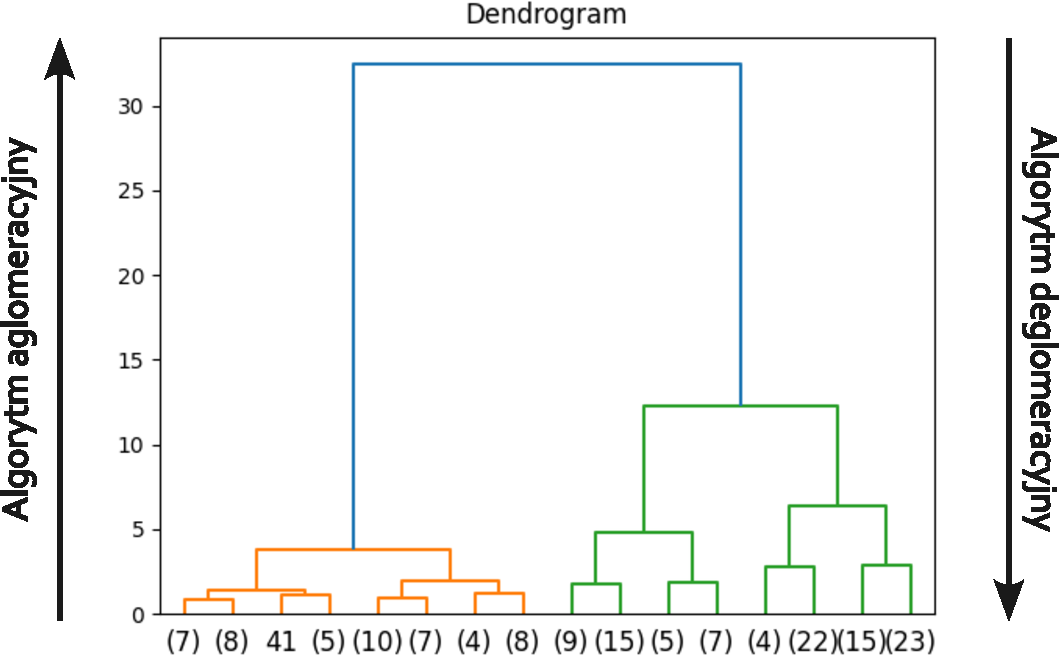
\includegraphics[width=\textwidth]{./dendrogram_iris.pdf}
\caption{Dendrogram otrzymany na podstawie grupowania hierarchicznego o łączności \english{single linkage} przykładowego zbioru danych \iris.}
\label{fig:dendrogram-iris}
\end{figure}

Często wybierana euklidesowa metryka odległości \cite{bib:hierarchical-overview} zdefiniowana jest jako
\begin{align}
	\Odleglosc_e \left(\wX_{i}, \wX_{j}\right) = \sqrt{\sum_{\Atrybut=0}^{\nAtrybut}(\X_{i\Atrybut} - \X_{j\Atrybut})^{2}},
	\label{eq:odleglosc:euklidesowa}
\end{align}
gdzie $\nAtrybut$ to liczba atrybutów punktu danych $\wX$, 
a $\X_{i\Atrybut}$ oznacza $\Atrybut$-ty atrybut $i$-tego punktu.
%
Metryka ta jest uszczegółowieniem metryki Minkowskiego
\begin{align}
\Odleglosc_m \left(\wX_{i}, \wX_{j}\right) = \left(\sum_{\Atrybut=0}^{\nAtrybut}|\X_{i\Atrybut} - \X_{j\Atrybut}|^{p}\right)^{1/p},
\end{align}
dla $p=2$. Inną popularną metryką jest odległość Manhattan, również należąca do rodziny metryk Minkowskiego, dla $p=1$.

Łączność określa, jak na podstawie odległości pomiędzy poszczególnymi punktami należącymi do klastrów wyznaczyć odległość pomiędzy tymi klastrami.
%
Do łączności zaimplementowanych w popularnych bibliotekach należą \english{single linkage} (najbliższe sąsiedztwo), \english{complete linkage} (najdalsze sąsiedztwo), \english{average linkage} (średnie sąsiedztwo) oraz metoda Warda (minimalna wariancja) \cite{bib:ward-linkage}.
%
Implementacje aglometacyjnego algorytmu hierarchicznego przedstawione są w \cite{bib:hierarchical-algorithms} Wykorzystywane one są przez bibliotekę \english{SciPy} języka Python \cite{bib:scipy-linkage}.

%przepisać, przekopiować pseudokody?
Algorytm naiwny (\PrimitiveClustering{}) może być wykorzystany dla każdej łączności, jednak jego wadą jest złożoność czasowa wynosząca $O(n^{3})$.
Jego parametrami wejściowymi są lista etykiet danych oraz macierz podobieństwa między danymi. W algorytmie naiwnym, iteracyjnie wykonywane są trzy kroki:
\begin{enumerate}
	\item Znalezienie w macierzy podobieństwa minimalnej wartości -- znalezienie najbliższej sobie pary klastrów,
	\item Scalenie odnalezionych klastrów,
	\item Aktualizacja wartości podobieństw w macierzy według wybranej łączności.
\end{enumerate}
Pseudokod działania algorytmu przedstawia alg. \ref{alg:primitive_clustering}.

\begin{algorithm}[t]
	\caption{Naiwny algorytm aglomeracyjnego grupowania hierarchicznego \PrimitiveClustering{} \cite{bib:hierarchical-algorithms}}
	\label{alg:primitive_clustering}
	\begin{algorithmic}[1]
		\Require $S$: etykiety elementów  \Comment{\ksremark{W rozdziale 3 inaczej oznaczamy etykiety.}}
		\Require $\mDistance$: macierz podobieństwa między każdą parą elementów 
		\Procedure{PrimitiveClustering}{$S, \mDistance$}
		\State $N \gets $ liczba elementów
		\State $L \gets [] $ \Comment{Lista wynikowa \ksremark{Co to znaczy?}}
		\State $rozmiar[x] \gets 1$ dla wszystkich $x \in S$  \Comment{\ksremark{for x in S ...}} \Comment{\ksremark{Czym jest rozmiar?}}
		\For{$i = 0$ to $N-2$} 
		\State $(a,b) \gets \arg\min_{(S \times S) \setminus \Delta}\mDistance$ \Comment{Operacja $\arg\min$ na macierzy $\mDistance$, uwzględniająca elementy ze zbioru $S$ z wyłączeniem przekątnej głównej}
		\State $S \gets S \setminus \{a, b\}$  \Comment{\ksremark{Trzeba skomentować.}}
		\State nowy element $n \notin S$  \Comment{\ksremark{To też trzeba skomentować.}}
		\For{$x$ in $S$}
		\State $\mDistance[n, x] \gets \mDistance[x, n] \gets $ \Call{UpdateFormula}{...} \Comment{wzór dla odpowiedniej łączności} \Comment{\ksremark{np. alg. \ref{alg:single_linkage}, alg. \ref{alg:complete_linkage}}}
		\EndFor
		\State $rozmiar[n] \gets rozmiar[a] + rozmiar[b]$
		\State $S \gets S \cup n$
		\EndFor
		\State \Return $L$  \Comment{\ksremark{Trzeba skomentować.}}
		\EndProcedure
	\end{algorithmic}
\end{algorithm}

Algorytm ogólny \texttt{GENERAL\_LINKAGE()} zawiera dodatkową optymalizację w stosunku do algorytmu naiwnego: wykorzystywana jest kolejka priorytetowa zawierająca kandydatów na najbliższych sąsiadów klastrów, co pozwala ograniczyć czas poszukiwania minimum macierzy w kroku 1. Optymistyczna złożoność czasowa tego algorytmu wynosi $\Omega(n^{2})$, pesymistyczna -- nadal $O(n^{3})$.

\subsection{Single Linkage}

Na czym polega
Wizualizacja, dendrogram
Typy implementacji (naiwna, SLINK...)

W algorytmie \SingleLinkage{} \cite{bib:hierarchical-clustering} odległość między klastrami jest równa minimalnej odległości między dwoma punktami należącymi do tych klastrów.
Oznacza to, że w momencie złączenia klastrów $A_{1}$ i $A_{2}$ w jeden klaster $A$, odległość tego klastra do innego klastra $B$ zdefiniowana jest jako:
\begin{align}
\Odleglosc \left(A, B\right) = \min(\Odleglosc(A_{1}, B), \Odleglosc(A_{2}, B)).
\end{align}

Wzór ten można przedstawić również w postaci pseudokodu \ref{alg:single_linkage}, którym uzupełnić można algorytm \ref{alg:primitive_clustering}.

\begin{algorithm}[t]
	\caption{Funkcja aktualizacji odległości między klastrami dla łączności \SingleLinkage{}}
	\label{alg:single_linkage}
	\begin{algorithmic}[1]
		\Require $d_{a, x}, d_{b, x}$: wartości odległości między klastrem $x$ a łączonymi w jeden klastrami $a$ i $b$
		\Procedure{UpdateFormula}{$d_{a, x}, d_{b, x}$}
		\State \Return $\min(d_{a, x}, d_{b, x})$
		\EndProcedure
	\end{algorithmic}
\end{algorithm}

%
Przykład takiego przypisania ilustruje rys. \ref{fig:single-linkage-example}. Odległość klastra $B$ od klastra $A_{1}$ jest znana i wynosi $\Odleglosc(A_{1}, B)$, czyli jest ona najmniejszą odległością między dowolnymi dwoma elementami klastrów $B$ i $A_{1}$. Odległość klastra $B$ od klastra $A_{2}$ również jest znana i wynosi $\Odleglosc(A_{2}, B)$. Klastry $A_{1}$ i $A_{2}$ scalane są w jeden klaster $A$, należy więc obliczyć odległość nowopowstałego klastra od pozostałych. Zamiast porównywać wszystkie możliwe kombinacje elementów klastrów $A$ i $B$, wystarczy znaleźć minimum z dwóch wartości: $\Odleglosc(A_{1}, B)$ i $\Odleglosc(A_{2}, B)$. W tym przypadku jest to odległość $\Odleglosc(A_{2}, B)$, czyli $\Odleglosc(A, B) = \Odleglosc(A_{2}, B)$
\ksremark{Trzeba tutaj opisać, co się na tym rysunku dzieje.}

%rysunek?
\begin{figure}
\centering
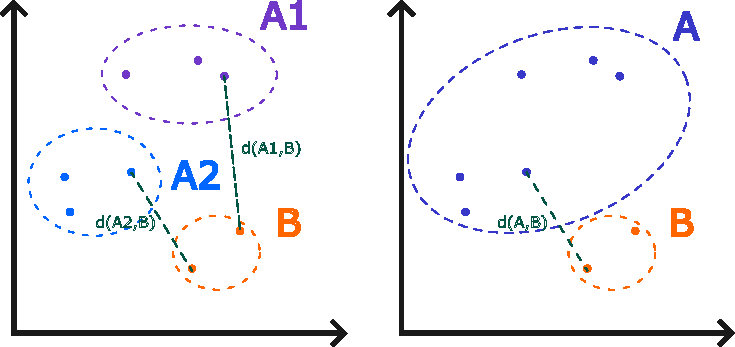
\includegraphics[width=\textwidth]{./single_linkage_example.pdf}
\caption{Ilustracja działania algorytmu \english{single linkage}. Odległość klastra $B$ od klastrów $A_{1}$ i $A_{2}$ jest znana. Po złączeniu $A_{1}$ i $A_{2}$ w klaster $A$, nowa odległość od klastra $B$ jest równa minimalnej z poprzednich dwóch -- w tym przypadku jest to odległość $\Odleglosc(A_{2}, B)$.}
\label{fig:single-linkage-example}
\end{figure}

Algorytm ten jest wrażliwy na szumy, dobrze działa dla wyraźnie oddzielonych klastrów.

Dla \english{single linkage} wykorzystać można szybsze, dedykowane algorytmy, na przykład algorytm minimalnego drzewa rozpinającego (\texttt{MST\_LINKAGE()}).


\ksremark{Więcej, trzeba napisać więcej!}

\subsection{Complete Linkage}

Algorytm \CompleteLinkage{} jest odwrotnością \SingleLinkage{}: odległość między klastrami jest równa maksymalnej odległości między dwoma punktami należącymi do tych klastrów. W momencie złączenia dwóch klastrów w jeden, jego odległość od pozostałych klastrów określa się więc jako:
\begin{align}
\Odleglosc \left(A, B\right) = \max(\Odleglosc(A_{1}, B), \Odleglosc(A_{2}, B)).
\end{align}

Wzór również można przedstawić jako pseudokod \ref{alg:complete_linkage}, uzupełniający algorytm \ref{alg:primitive_clustering}.

\begin{algorithm}[t]
	\caption{Funkcja aktualizacji odległości między klastrami dla łączności \CompleteLinkage{}}
	\label{alg:complete_linkage}
	\begin{algorithmic}[1]
		\Require $d_{a, x}, d_{b, x}$: wartości odległości między klastrem $x$ a łączonymi w jeden klastrami $a$ i $b$
		\Procedure{UpdateFormula}{$d_{a, x}, d_{b, x}$}
		\State \Return $\max(d_{a, x}, d_{b, x})$
		\EndProcedure
	\end{algorithmic}
\end{algorithm}
%
Algorytm dobrze działa dla kulistych, gęstych klastrów, ale w porównaniu z \SingleLinkage{} zwraca gorsze wyniki dla danych o innych kształtach \cite{bib:hierarchical-clustering, bib:sklearn-linkage-comparison}.

\ksremark{Trzeba napisać jeszcze, jaka jest różnica w wynikach \SingleLinkage\ i complete.}

\section{Algorytm rozmytych $c$ średnich}
\label{sec:fcm}

Algorytm rozmytych $c$ średnich (ang. \english{fuzzy $c$-means}, FCM) należy do rodziny algorytmów opartych o minimalizację funkcji kryterialnej. Algorytm wyznacza klastry, dla których przynależność każdego punktu danych jest liczbą z przedziału $\left[ 0,1 \right]$. Wynikiem klasteryzacji FCM jest macierz środków klastrów $\mCentre$ oraz macierz przynależności $\mClusterMembership$. Złożoność czasowa ze względu na liczbę danych tego algorytmu wynosi $O(n)$ \cite{bib:fcm-kmeans-comparison}.

Funkcja kryterialna algorytmu fuzzy c-means ma postać:
\begin{align}
	J(\mCentre, \mClusterMembership) = \sum_{\Iteracja=1}^{N} \sum_{\Klaster=1}^{\nKlaster}\ClusterMembership_{\Iteracja\klaster}^{m} ||\wX_{\Iteracja} - \wCentre_{\klaster}||^{m},
\end{align}
%\sum_{\size=1}^{\nSize}  \sum_{\Klaster=1}^{\nKlaster}\ClusterMembership_{\size\klaster}^{m}
%nie działa z \nSize ani \nLen
gdzie $\wX_{\Iteracja}$ -- współrzędne $\Iteracja$-tego punktu danych, $\wCentre_{\klaster}$ -- współrzędne środka $\klaster$-tego klastra danych, $\ClusterMembership_{\Iteracja\klaster} \in \left[ 0,1 \right]$ -- wartość przynależności $\Iteracja$-tego punktu do $\klaster$-tego klastra. Parametr $m \in \left( 1,+\infty \right]$ jest współczynnikiem rozmycia algorytmu, najczęściej wykorzystuje się wartość 2 \cite{bib:implementation-of-fcm-pcm-algs,bib:scikit-fuzzy-cmeans-docs-fcm}.

Dla każdego punktu, suma jego wartości przynależności do wszystkich klastrów wynosi 1:

\begin{align}
	\label{eq:cluster_mem_condition}
	\forall \Iteracja \in [1, N] \sum_{\Klaster=1}^{\nKlaster}\ClusterMembership_{\Iteracja\klaster} = 1
\end{align}

W każdej iteracji algorytmu obliczane są najpierw nowe współrzędne środków klastrów:
\begin{align}
	\label{eq:center_update}
	\wCentre_{\klaster} = \frac{\sum_{\Iteracja=1}^{N} \ClusterMembership_{\Iteracja\klaster}^{m} \wX_{\Iteracja}}{\sum_{\Iteracja=1}^{N} \ClusterMembership_{\Iteracja\klaster}^{m}},
\end{align}
a następnie wartości elementów macierzy przynależności:
\begin{align}
	\label{eq:membership_update}
	\ClusterMembership_{\Iteracja\klaster} = \frac{1}{\sum_{j=1}^{\nKlaster}\left( \frac{||\wX_{\Iteracja} - \wCentre_{\klaster}||}{||\wX_{\Iteracja} - \wCentre_{j}||} \right)^{\frac{2}{m - 1}}}.
\end{align}
Kroki powtarzane są do momentu spełnienia warunku zatrzymania, na przykład:
\begin{align}
	\label{eq:fcm_stop_contidion}
	||\mClusterMembership^{(t)} - \mClusterMembership^{(t-1)}|| < \epsilon,
\end{align}
%
gdzie $t$ -- numer iteracji, $\epsilon$ -- parametr tolerancji. Dodatkowym warunkiem zatrzymania może też być z góry określona maksymalna liczba iteracji \cite{bib:scikit-fuzzy-cmeans-docs-fcm, bib:skfuzzy-docs-fcm}.

\begin{algorithm}[t]
	\caption{Algorytm rozmytych $c$ średnich}
	\label{alg:fcm}
	\begin{algorithmic}[1]
		\Require $\zX$: dane do klasteryzacji
		\Require $\nKlaster$: liczba klastrów docelowych
		\Require $m$: współczynnik rozmycia 
		\Require $\nIteracja$: maksymalna liczba iteracji
		\Require $\varepsilon$: tolerancja
		\Procedure{FuzzyCMeans}{$\zX, \nKlaster, m, \nIteracja, \varepsilon$}
		\State $\nX \gets $ liczba próbek
		\State $\nAtrybut \gets $ liczba atrybutów \Comment{$\nX$ i $\nAtrybut$: wymiary $\zX$} 
		\State $\wCentre \gets $ losowe wartości początkowe środków klastrów
		\State $U \gets $ losowe wartości początkowe przynależności punktów do klastrów, spełniające warunek ze wzoru \ref{eq:cluster_mem_condition} \Comment{\ksremark{$\mMembership$}}
		\State $i\gets 1$
		\State koniec $\gets$ false
		\While{$i < \nIteracja$ $\land$ $\lnot$ koniec} 
		\State aktualizacja wartości $\wCentre$ na podstawie wzoru \ref{eq:center_update} \Comment{\ksremark{Dla wzorów zawsze używamy eqref zamiast ref.}}
		\State aktualizacja wartości $\mMembership$ na podstawie wzoru \ref{eq:membership_update}
		\If{spełniony warunek \ref{eq:fcm_stop_contidion}}
		\State  koniec $\gets$ true
		\EndIf
		\EndWhile
		\State \Return $v, U$
		\EndProcedure
	\end{algorithmic}
\end{algorithm}

\section{Obliczenia ziarniste}

\ksremark{zagajenie}

Obliczenia ziarniste (granularne) pozwalają na analizę danych w bardziej zbliżony do ludzkiego sposób zrozumienia. 

\subsection{Ziarna informacyjne}
\ksremark{Co to jest?}
\ksremark{Jak są reprezentowane?}
\ksremark{Jak się tworzy ziarna obliczeniowe?}

Jednym z podstawowych pojęć związanych z obliczeniami ziarnistymi są ziarna informacyjne. 
Są one encjami o pewnej semantyce, kolekcjami obiektów o określonym w~pewien sposób podobieństwie \cite{bib:general-framework-information-granules,bib:designing-higher-order-information-granules}.
%
W zależności od znaczenia i zastosowania ziaren, mogą one być reprezentowane na różne sposoby: jako zbiory klasyczne, przedziały liczb, zbiory rozmyte, zbiory cieniowane, zbiory przybliżone, czy funkcje prawdopodobieństwa \cite{bib:general-framework-information-granules}.
%
Ziarna informacyjne utworzyć można poprzez grupowanie danych. W przypadku ziaren reprezentowanych przez zbiory rozmyte, typowym algorytmem grupowania jest algorytm rozmytych $c$-średnich \ref{sec:fcm}.
% TODO link do rozdziału o FCM

\subsection{Zbiory rozmyte}

Zbiory klasyczne są pojęciem pierwotnym: obiekt $\X$ (liczba, punkt, dana itp.) należy do zbioru $\zA$ ($\X \in \zA$) lub do niego nie należy ($\X \notin \zA$). 

W przypadku zbiorów rozmytych, obiekt $\X$ należy do zbioru $\zA$ z pewnym stopniem przynależności z przedziału $\left[ 0,1 \right]$, gdzie 0 oznacza całkowity brak przynależności, a 1 -- całkowitą przynależność \cite{bib:introduction-to-fuzzy-sets}. Zbiór rozmyty $\zA$ opisać można poprzez funkcję przynależności $\ClusterMembership_{\zA}: \zX \to \left[ 0,1 \right]$.

Dla zbioru rozmytego można wyróżnić jego rdzeń oraz nośnik:

\begin{Definition}
	\cite{bib:introduction-to-fuzzy-sets} Rdzeń zbioru rozmytego $\zA$ to taki jego podzbiór $\zA_{C}$, dla którego $\ClusterMembership_{\zA_{C}} = 1$.
\end{Definition}

\begin{Definition}
	\cite{bib:introduction-to-fuzzy-sets} Nośnik zbioru rozmytego $\zA$ to taki jego podzbiór $\zA_{S}$, dla którego $\ClusterMembership_{\zA_{S}} > 0$.
\end{Definition}

Graficzną interpretację tych charakterystyk przedstawiono na rys. \ref{fig:core-support-example}. Zbiór rozmyty może nie posiadać rdzenia ($\forall_{\X \in \zA}\;  \ClusterMembership(\X)_{\zA} < 1$), może mieć nieskończony nośnik ($\forall_{\X \in \zA}\;  \ClusterMembership(\X)_{\zA} > 0$).

\begin{figure}
\centering
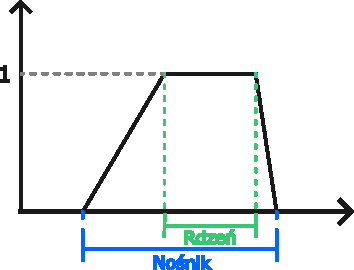
\includegraphics[width=\textwidth]{./core_support_example.pdf}
\caption{Wykres trapezowego zbioru rozmytego, ilustrujący jego rdzeń i nośnik.}
\label{fig:core-support-example}
\end{figure}

\subsubsection{Operacje na zbiorach rozmytych}

Podstawowymi operacjami na zbiorach klasycznych są iloczyn i suma. Ich odpowiednikami dla zbiorów rozmytych są odpowiednio t-norma ($\star_T$) i s-norma ($\star_S$), które spełniają warunki określone w tabeli \ref{id:tab:tnorm-snorm}.

\begin{table}
\centering
\caption{Warunki t-norm i s-norm}
\label{id:tab:tnorm-snorm}
\begin{tabular}{lll}
\toprule
	& t-norma & s-norma  \\
\midrule
	    warunki graniczne & $x \star_T 1 = x, x \star_T 0 = 0$ & $x \star_S 1 = 1, x \star_S 0 = x$ \\
	    przemienność & $x \star_T y = y \star_T x$ & $x \star_S y = y \star_S x$ \\
		monotoniczność & jeżeli $x \le u$ to $x \star_T y \le u \star_T y$,  & jeżeli $x \le u$ to $x \star_S y \le u \star_S y$,\\ 
		& jeżeli $y \le r$ to $x \star_T y \le x \star_T r$ & jeżeli $y \le r$ to $x \star_S y \le x \star_S r$ \\
	    łączność & $x \star_T (y \star_T z) = (x \star_T y) \star_T z$ & $x \star_S (y \star_S z) = (x \star_S y) \star_S z$ \\
\bottomrule
\end{tabular}
\end{table}  

Istnieje wiele t-norm i s-norm spełniających te warunki. W ramach tej pracy, najistotniejsze są:

\begin{itemize}
	\item t-norma i s-norma algebraiczna:
	\begin{align}
		\label{eq:algebraic-norms}
		x \star_T y = xy \\
		x \star_S y = x + y - xy
	\end{align}
	\item t-norma i s-norma Łukasiewicza:
	\begin{align}
		x \star_T y = \max(x + y - 1, 0) \\
		x \star_S y = \min(x + y, 1)
	\end{align}
\end{itemize}

Inną typową operacją na zbiorach rozmytych jest negacja. Musi ona spełniać warunki $\bar{0} = 1, \bar{1} = 0, x \le y \Rightarrow \bar{x} \ge \bar{y}$ \cite{bib:mathematics-fuzzy-sets-logic}. Najczęściej wykorzystywaną negacją jest negacja standardowa:
\begin{align}
	\bar{x} = 1 - x
\end{align}

Jest to negacja silna, czyli spełnia ona również warunek $\bar{\bar{x}} = x$.

\subsection{Rozszerzalne liczby rozmyte}
\label{sec:rozszerzalne-liczby-rozmyte}
\ksremark{Liczby rozmyte}
\ksremark{Kształty (trójkątne, wykładnicze, gaussowskie)}
\ksremark{Relacje między liczbami (arytmetyka, porównanie)}

Rozszerzalne liczby rozmyte (ang. \english{extensional fuzzy numbers}) są uogólnieniem liczb rzeczywistych. Są to zbiory rozmyte, które modelują semantykę taką, jak ,,około 5'', ,,prawie 10'', ,,ponad 20'', czyli odpowiadają rzeczywistym liczbom ostrym z pewną tolerancją \cite{bib:arithmetics-extensional-fuzzy-numbers,bib:mathematics-fuzzy-sets-logic}. Definiowana jest dla nich rozmyta relacja $\ast$-podobieństwa $\nPodobienstwo$.

\begin{Definition}
\label{def:fuzzy-similarity}
	\cite{bib:arithmetics-extensional-fuzzy-numbers} Rozmyta relacja $\ast$-podobieństwa $\nPodobienstwo(\X,\Y)$, gdzie $\ast$ jest lewostronnie ciągłą t-normą, spełnia warunki:
	\begin{align}
		\nPodobienstwo(\X,\X) & = 1 \\
		\nPodobienstwo(\X,\Y) & = \nPodobienstwo(\Y,\X)\\
		\nPodobienstwo(\X,\Y) & \ast \nPodobienstwo(\Y,\Z) \leqslant \nPodobienstwo(\X,\Z)
	\end{align}
\end{Definition}

Rozszerzalne liczby rozmyte to liczby ostre rozszerzone o relację $\ast$-podobieństwa. Dla dowolnego $\Y \in \zRzeczywista$ liczbę rozmytą można przedstawić jako \cite{bib:arithmetics-extensional-fuzzy-numbers}:
\begin{align}
	\X_{\nPodobienstwo}(\Y) = \nPodobienstwo(\X, \Y)
\end{align}

\subsubsection{Kształty liczb rozmytych}
\label{sec:ksztalty-liczb-rozmytych}

Kształt rozszerzalnej liczby rozmytej określony jest przez relację $\ast$-podobieństwa. Może on być dowolny, o ile spełnia warunki określone w definicji \ref{def:fuzzy-similarity}. W pracy wykorzystywane są trzy kształty, opisane w \cite{bib:fuzzy-numbers-revisited-logic-operations}:

\paragraph{Liczby trójkątne}

Dla liczb trójkątnych relacja $\ast$-podobieństwa $\nPodobienstwo_{t}$ definiowana jest jako:
\begin{align}
	\label{eq:similarity_t}
	\nPodobienstwo_{t}(\X,\Y) = \max \left\{1 - \frac{|\X-\Y|}{p}, 0 \right\},
\end{align}
gdzie $p > 0$, a $\ast$ to t-norma Łukasiewicza.

\paragraph{Liczby wykładnicze}

Dla liczb wykładniczych relacja $\ast$-podobieństwa $\nPodobienstwo_{e}$ definiowana jest jako:
\begin{align}
	\label{eq:similarity_e}
	\nPodobienstwo_{e}(\X,\Y) = \exp \left(- \frac{|\X-\Y|}{p} \right),
\end{align}
gdzie $p > 1$, a $\ast$ to t-norma iloczynowa.

\paragraph{Liczby gaussowskie}

Dla liczb gaussowskich relacja $\ast$-podobieństwa $\nPodobienstwo_{g}$ definiowana jest jako:
\begin{align}
	\label{eq:similarity_g}
	\nPodobienstwo_{g}(\X,\Y) = \exp \left(- \frac{(\X-\Y)^{2}}{2p^{2}} \right),
\end{align}
gdzie $p > 0$, a $\ast$ to t-norma iloczynowa.

\subsubsection{Operacje arytmetyczne}

Operacje arytmetyczne na rozszerzalnych liczbach rozmytych są proste obliczeniowo i nie zwiększają rozmycia. Wynikiem operacji arytmetycznej na rozszerzalnej liczbie lub liczbach rozmytych jest rozszerzalna liczba rozmyta.

Operacje arytmetyczne jednoargumentowe można zapisać w ogólny sposób jako:
\begin{align}
	\mathbf{op}(\X_{\nPodobienstwo}) = \mathbf{op}(\X)_{\nPodobienstwo},
\end{align}
na przykład:
\begin{align}
	(\X_{\nPodobienstwo})^{2} = (\X^{2})_{\nPodobienstwo}.
\end{align}

Operacje arytmetyczne dwuargumentowe można zapisać jako:
\begin{align}
	\X_{\nPodobienstwo_{\X}} \; \mathbf{op} \; \Y_{\nPodobienstwo_{\Y}} = (\X \; \mathbf{op} \; \Y)_{cl(\nPodobienstwo_{\X} \cup \nPodobienstwo_{\Y})},
\end{align}
gdzie $cl(\nPodobienstwo_{\X} \cup \nPodobienstwo_{\Y})$ jest domknięciem relacji $\nPodobienstwo_{\X}$ i $\nPodobienstwo_{\Y}$. Dla zdefiniowanych w podsekcji \ref{sec:ksztalty-liczb-rozmytych} kształtów ($\nPodobienstwo \in \{ \nPodobienstwo_{t}, \nPodobienstwo_{e}, \nPodobienstwo_{g}\}$) przyjąć można, że
\begin{align}
	cl(\nPodobienstwo(p_{\X}) \cup \nPodobienstwo(p_{\Y})) = \max\{p_{\X}, p_{\Y}\}.
\end{align}

Przykładowo, odległość euklidesową między dwoma punktami, będącymi dwuwymiarowymi trójkątnymi liczbami rozmytymi, zapisać można jako:
\begin{multline}
	\Odleglosc ((5_{\nPodobienstwo_{t}(2,5)}, -2_{\nPodobienstwo_{t}(0,5)}), (8_{\nPodobienstwo_{t}(1,25)}, 2_{\nPodobienstwo_{t}(4)})) = \\
	= \sqrt{(5_{\nPodobienstwo_{t}(2,5)} - 8_{\nPodobienstwo_{t}(1,25)})^{2} + (-2_{\nPodobienstwo_{t}(0,5)} - 2_{\nPodobienstwo_{t}(4)})^{2}} = 5_{\nPodobienstwo_{t}(4)}.
\end{multline}

\subsubsection{Operacje logiczne}
Operacje porównania na rozszerzalnych liczbach rozmytych oparte są o operator równości rozmytej \cite{bib:fuzzy-numbers-revisited-logic-operations}:
\begin{Definition}
	Operator równości rozmytej $=_{\nPodobienstwo}: \zRozszerzalna \times \zRozszerzalna \to [0,1]$ zdefiniowany jest przy pomocy rozmytej relacji $\ast$-podobieństwa $\nPodobienstwo$:
	\begin{align}
		\label{eq:fuzzy-equality}
		\left(\X_{\nPodobienstwo(p_{\X})} =_{\nPodobienstwo} \Y_{\nPodobienstwo(p_{\Y})}\right) = \nPodobienstwo_{\max\{p_{\X},p_{\Y}\}}(\X, \Y)
	\end{align}
\end{Definition}

Przykładowo, dla liczb z relacją trójkątną:
\begin{align}
	\left(\X_{\nPodobienstwo_{t}(p_{\X})} =_{\nPodobienstwo} \Y_{\nPodobienstwo_{t}(p_{\Y})}\right) = \max \left\{1 - \frac{|\X-\Y|}{\max\{p_{\X},p_{\Y}\}}, 0 \right\}
\end{align}

Operatory nierówności wyznaczane są w następujący sposób:

\begin{align}
	\left(\X_{\nPodobienstwo(p_{\X})} <_{\nPodobienstwo} \Y_{\nPodobienstwo(p_{\Y})}\right) = \left\{ \begin{array}{cl}
	1 -  \left(\X_{\nPodobienstwo(p_{\X})} =_{\nPodobienstwo} \Y_{\nPodobienstwo(p_{\Y})}\right) & : \  \X \le \Y \\
	0 & : \ \X > \Y
	\end{array} \right.
\end{align}

\begin{align}
	\left(\X_{\nPodobienstwo(p_{\X})} \le_{\nPodobienstwo} \Y_{\nPodobienstwo(p_{\Y})}\right) = \left\{ \begin{array}{cl}
	1 & : \  \X \le \Y \\
	\left(\X_{\nPodobienstwo(p_{\X})} =_{\nPodobienstwo} \Y_{\nPodobienstwo(p_{\Y})}\right) & : \ \X > \Y
	\end{array} \right.
\end{align}

\begin{align}
	\left(\X_{\nPodobienstwo(p_{\X})} >_{\nPodobienstwo} \Y_{\nPodobienstwo(p_{\Y})}\right) = \left\{ \begin{array}{cl}
	1 -  \left(\X_{\nPodobienstwo(p_{\X})} =_{\nPodobienstwo} \Y_{\nPodobienstwo(p_{\Y})}\right) & : \  \X \ge \Y \\
	0 & : \ \X < \Y
	\end{array} \right.
\end{align}

\begin{align}
	\left(\X_{\nPodobienstwo(p_{\X})} \ge_{\nPodobienstwo} \Y_{\nPodobienstwo(p_{\Y})}\right) = \left\{ \begin{array}{cl}
	1 & : \  \X \ge \Y \\
	\left(\X_{\nPodobienstwo(p_{\X})} =_{\nPodobienstwo} \Y_{\nPodobienstwo(p_{\Y})}\right) & : \ \X < \Y
	\end{array} \right.
\end{align}


% TODO

% \chapter{[Tytuł rozdziału]} 

% tekst

% \section{[Tytuł podrozdziału]}

% \section{[Tytuł podrozdziału]}

% W całym dokumencie powinny znajdować się odniesienia do zawartych w nim ilustracji (rys. \ref{fig:2}).

% \begin{figure}
% \centering
% \begin{tikzpicture}
% \begin{axis}[
%     y tick label style={
%         /pgf/number format/.cd,
%             fixed,   % po zakomentowaniu os rzednych jest indeksowana wykladniczo
%             fixed zerofill, % 1.0 zamiast 1
%             precision=1,
%         /tikz/.cd
%     },
%     x tick label style={
%         /pgf/number format/.cd,
%             fixed,
%             fixed zerofill,
%             precision=2,
%         /tikz/.cd
%     }
% ]
% \addplot [domain=0.0:0.1] {rnd};
% \end{axis} 
% \end{tikzpicture}
% \caption{Wykres przebiegu funkcji.} % Podpis jest zawsze POD rysunkiem.
% \label{fig:2}
% \end{figure}


%%%%%%%%%%%%%%%%%%%%%
%% RYSUNEK Z PLIKU
%
%\begin{figure}
%\centering
%\includegraphics[width=0.5\textwidth]{./politechnika_sl_logo_bw_pion_pl.pdf}
%\caption{Podpis rysunku zawsze pod rysunkiem.}
%\label{fig:etykieta-rysunku}
%\end{figure}
%Rys. \ref{fig:etykieta-rysunku} przestawia …
%%%%%%%%%%%%%%%%%%%%%
%
%%%%%%%%%%%%%%%%%%%%%
%% WIELE RYSUNKÓW 
%
%\begin{figure}
%\centering
%\begin{subfigure}{0.4\textwidth}
%    \includegraphics[width=\textwidth]{./politechnika_sl_logo_bw_pion_pl.pdf}
%    \caption{Lewy górny rysunek.}
%    \label{fig:lewy-gorny}
%\end{subfigure}
%\hfill
%\begin{subfigure}{0.4\textwidth}
%    \includegraphics[width=\textwidth]{./politechnika_sl_logo_bw_pion_pl.pdf}
%    \caption{Prawy górny rysunek.}
%    \label{fig:prawy-gorny}
%\end{subfigure}
%
%\begin{subfigure}{0.4\textwidth}
%    \includegraphics[width=\textwidth]{./politechnika_sl_logo_bw_pion_pl.pdf}
%    \caption{Lewy dolny rysunek.}
%    \label{fig:lewy-dolny}
%\end{subfigure}
%\hfill
%\begin{subfigure}{0.4\textwidth}
%    \includegraphics[width=\textwidth]{./politechnika_sl_logo_bw_pion_pl.pdf}
%    \caption{Prawy dolny rysunek.}
%    \label{fig:prawy-dolny}
%\end{subfigure}
%        
%\caption{Wspólny podpis kilku rysunków.}
%\label{fig:wiele-rysunkow}
%\end{figure}
%Rys. \ref{fig:wiele-rysunkow} przestawia wiele ważnych informacji, np. rys. \ref{fig:prawy-gorny} jest na prawo u góry.
%%%%%%%%%%%%%%%%%%%%%


% Tekst dokumentu powinien również zawierać odniesienia do tabel (tab. \ref{id:tab:wyniki}).

% \begin{table}
% \centering
% \caption{Opis tabeli nad nią.}
% \label{id:tab:wyniki}
% \begin{tabular}{rrrrrrrr}
% \toprule
% 	         &                                     \multicolumn{7}{c}{metoda}                                      \\
% 	         \cmidrule{2-8}
% 	         &         &         &        \multicolumn{3}{c}{alg. 3}        & \multicolumn{2}{c}{alg. 4, $\gamma = 2$} \\
% 	         \cmidrule(r){4-6}\cmidrule(r){7-8}
% 	$\zeta$ &     alg. 1 &   alg. 2 & $\alpha= 1.5$ & $\alpha= 2$ & $\alpha= 3$ &   $\beta = 0.1$  &   $\beta = -0.1$ \\
% \midrule
% 	       0 &  8.3250 & 1.45305 &       7.5791 &    14.8517 &    20.0028 & 1.16396 &                       1.1365 \\
% 	       5 &  0.6111 & 2.27126 &       6.9952 &    13.8560 &    18.6064 & 1.18659 &                       1.1630 \\
% 	      10 & 11.6126 & 2.69218 &       6.2520 &    12.5202 &    16.8278 & 1.23180 &                       1.2045 \\
% 	      15 &  0.5665 & 2.95046 &       5.7753 &    11.4588 &    15.4837 & 1.25131 &                       1.2614 \\
% 	      20 & 15.8728 & 3.07225 &       5.3071 &    10.3935 &    13.8738 & 1.25307 &                       1.2217 \\
% 	      25 &  0.9791 & 3.19034 &       5.4575 &     9.9533 &    13.0721 & 1.27104 &                       1.2640 \\
% 	      30 &  2.0228 & 3.27474 &       5.7461 &     9.7164 &    12.2637 & 1.33404 &                       1.3209 \\
% 	      35 & 13.4210 & 3.36086 &       6.6735 &    10.0442 &    12.0270 & 1.35385 &                       1.3059 \\
% 	      40 & 13.2226 & 3.36420 &       7.7248 &    10.4495 &    12.0379 & 1.34919 &                       1.2768 \\
% 	      45 & 12.8445 & 3.47436 &       8.5539 &    10.8552 &    12.2773 & 1.42303 &                       1.4362 \\
% 	      50 & 12.9245 & 3.58228 &       9.2702 &    11.2183 &    12.3990 & 1.40922 &                       1.3724 \\
% \bottomrule
% \end{tabular}
% \end{table}  

\chapter{Rozmyty algorytm aglomeracyjnego grupowania hierarchicznego}

%\begin{itemize}
%\item  Jak ja rozwiązuję problem?
%\begin{itemize}
%\item rozwiązanie zaproponowane przez dyplomanta
%\item analiza teoretyczna rozwiązania
%\item uzasadnienie wyboru zastosowanych metod, algorytmów, narzędzi
%\end{itemize}
%\end{itemize}

%\section{Plan rozwiązania}

Problemem algorytmów grupowania hierarchicznego jest ich duża złożoność czasowa -- w przypadku algorytmu ogólnego aż do $O(n^{3})$. Zmniejszenie liczby danych poprzez zastosowanie wstępnej granulacji algorytmem rozmytych $c$-średnich może znacznie przyspieszyć jego działanie, jako że algorytm ten ma stałą złożoność czasową w zależności od liczby danych. \ksremark{Napisałbym tutaj, że ma złożoność $O(\nGranula^3)$, ale $\nGranula \ll n$.}

Rozmyty algorytm aglomeracyjnego grupowania hierarchicznego \MojAlg\ składa się z trzech głównych kroków:

\begin{enumerate}
	\item granulacja oryginalnych danych przy pomocy algorytmu rozmytych $c$-średnich (roz. \ref{sec:granulacja-danych-oryginalnych}),
	\item przekształcenie otrzymanych wyników w granule o potrzebnych parametrach (roz. \ref{sec:granulacja-danych-oryginalnych} \ksremark{¿czy na pewno}),
	\item aglomeracyjne grupowanie hierarchiczne granul z uwzględnieniem ich rozmycia: \MojHierAlg\ (roz. \ref{sec:granulacja-danych-oryginalnych} \ksremark{¿czy na pewno}).
\end{enumerate}

Złożoność czasowa tego algorytmu może zostać określona jako $O(n + \nGranula^3)$, przy czym $\nGranula \ll n$ odpowiada liczbie granul.

\section{Granulacja danych oryginalnych}
\label{sec:granulacja-danych-oryginalnych}

W pierwszym kroku oryginalne dane są granulowane przez algorytm rozmytych $c$-średnich. Dane mają postać macierzy liczb rzeczywistych o wymiarach $\nX \times \nAtrybut$, gdzie $\nX$ -- liczba danych, $\nAtrybut$ -- liczba atrybutów. Wartość parametru rozmycia $m$ algorytmu określona jest na stałe jako 2. Liczba docelowych klastrów $\nKlaster$ jest jednym z parametrów badawczych i jest znacznie mniejsza od $\nX$.

\section{Przekształcenie granul}

Granule wykorzystywane do grupowania hierarchicznego mają postać wielowymiarowych rozszerzalnych liczb rozmytych. Dla każdego wymiaru musi zostać określona wartość ostra liczby $x$ oraz jej rozmycie $p$.

Wartości ostre są tożsame ze środkami klastrów będących wynikiem algorytmu rozmytych $c$-średnich, czyli z wektorem $\wCentre$ (wzór \ref{eq:center_update}).

Wartościom rozmycia nie odpowiada bezpośrednio żadna ze struktur zwracanych przez FCM. Dla każdego klastra $\Klaster$ i wymiaru (atrybutu) $\Atrybut$, rozmycie oblicza się jako następującą wariancję:
\begin{align}
	p_{\Klaster \Atrybut} = \sqrt{\frac{\sum_{\Iteracja = 1}^{\nX} \ClusterMembership_{\klaster\Iteracja}^{m} (\X_{\Iteracja\Atrybut} - \Centre_{\Klaster\Atrybut})^{2}}{\sum_{\Iteracja = 1}^{\nX} \ClusterMembership_{\klaster\Iteracja}^{m}}}.
\end{align}

Granule nie mają na stałe określonego kształtu rozszerzalnych liczb rozmytych, które składają się na ich wymiary. Kształt jest więc parametrem dla operacji logicznych na nich wykonywanych.

\subsection{Rozmyte grupowanie hierarchiczne}

Zbiór granul $\zGranula$ oraz ich kształt są parametrami wejściowymi algorytmu rozmytego aglomeracyjnego grupowania hierarchicznego \MojHierAlg.
%
Na początku wyznaczane są rozmyte odległości euklidesowe (wzór \eqref{eq:odleglosc:euklidesowa})między każdą parą granul, przy pomocy operacji arytmetycznych określonych w sekcji \ref{sec:rozszerzalne-liczby-rozmyte}. Wynikiem obliczeń jest symetryczna macierz odległości $\mDistance$ o wymiarach $\nX \times \nX$, gdzie $\Distance_{ij} = \Distance_{ji} = \Distance(\wX_{i}, \wX_{j})$.

Grupowanie hierarchiczne \MojHierAlg{} ma postać zmodyfikowanego algorytmu naiwnego \PrimitiveClustering{}, o złożoności czasowej $O(\nGranula^{3})$. Zmieniony musi zostać sposób wyznaczania kolejnych minimalnych odległości w macierzy $\mDistance$ oraz, zależne od łączności, aktualizacje odległości do nowo scalonego klastra. 

Minimum i maksimum wyznacza się przy pomocy operacji porównania. W przypadku rozszerzalnych liczb rozmytych, wynikami takich operacji są liczby z przedziału $[0, 1]$. W celu określenia, która z liczb rozmytych jest większa lub mniejsza, wprowadzony zostaje parametr $\xi$, będący parametrem badawczym. Algorytmy rozmytego minimum i maksimum przedstawiają odpowiednio pseudokody \ref{alg:fuzzy-min} i \ref{alg:fuzzy-max}. Na podstawie alg. \ref{alg:fuzzy-min} można też utworzyć rozmytą funkcję $\arg\min$ (alg. \ref{alg:fuzzy-argmin}).

Dla łączności \SingleLinkage{}, algorytm \MojHierAlg{} ma postać opisaną pseudokodem \ref{alg:fuzzy_single_linkage}.

\begin{algorithm}[t]
	\caption{Minimum rozmyte}
	\label{alg:fuzzy-min}
	\begin{algorithmic}[1]
		\Require $a, b$: porównywane rozszerzalne liczby rozmyte
		\Require $r$: typ relacji (trójkątna, wykładnicza, gaussowska)
		\Require $\xi$: parametr porównania \ksremark{To trzeba będzie chyba nazwać jakoś inaczej.}
		\Procedure{FuzzyMinimum}{$a, b, r, \xi$}
		\If{$(a <_{\nPodobienstwo_r} b) > \xi$}
		\State \Return $a$
		\Else
		\State \Return $b$
		\EndIf
		\EndProcedure
	\end{algorithmic}
\end{algorithm}

\begin{algorithm}[t]
	\caption{Maksimum rozmyte}
	\label{alg:fuzzy-max}
	\begin{algorithmic}[1]
		\Require $a, b$: porównywane rozszerzalne liczby rozmyte, $r$: typ relacji (trójkątna, wykładnicza, gaussowska), $\xi$: parametr porównania \ksremark{Trzeba rozbić parametry jak w alg. \ref{alg:fuzzy-min}.}
		\Procedure{FuzzyMaximum}{$a, b, r, \xi$}
		\If{$(a >_{\nPodobienstwo_r} b) > \xi$}
		\State \Return $a$
		\Else
		\State \Return $b$
		\EndIf
		\EndProcedure
	\end{algorithmic}
\end{algorithm}

\begin{algorithm}[t]
	\caption{Rozmyta funkcja $\arg\min$}
	\label{alg:fuzzy-argmin}
	\begin{algorithmic}[1]
		\Require $\mX$: macierz liczb rozmytych, $\wPunkt$: wektor indeksów, dla których znajdowane jest minimum, $r$: typ relacji (trójkątna, wykładnicza, gaussowska), $\xi$: parametr porównania 
		\Procedure{FuzzyArgMin}{$\mX, r, \xi$}
		\State result $\gets \infty_{S(0)}$  \Comment{liczba rozmyta, dla której $x=\infty, p=0$}
		\State $(w, k) \gets (0, 0)$  \Comment{\ksremark{Trzeba to skomentować.}}
		\For{$i = 1$ to $\nPunkt - 1$} \Comment{\ksremark{Trzeba napisać, co oznacza $\nPunkt$. Może zamiast $\nPunkt$ użyć $|\wPunkt|$?}}
		\For{$j = i + 1$ to $\nPunkt$}
		\State $p_i, p_j \gets \wPunkt[i], \wPunkt[j]$   \Comment{\ksremark{Rozbiłbym to na dwie instrukcje.}}
		\If{($\mX[p_i, p_j] <_{\nPodobienstwo_r}$ result) > $\xi$}\Comment{\ksremark{Trzeba napisać $\mX[p_i][p_j]$}.}
		\State result $\gets \mX[p_i, p_j]$
		\State $(w, k) \gets (p_i, p_j)$ \Comment{\ksremark{Skoro mamy takie przypisanie, to może zamiast $i$ użyć $w$ i zamiast $j$ – $k$?}}
		\EndIf
		\EndFor
		\EndFor
		\State \Return $(w, k)$  \Comment{\ksremark{Tu napiszemy, co zwracamy.}}
		\EndProcedure
	\end{algorithmic}
\end{algorithm}

\begin{algorithm}[t]
	\caption{Algorytm rozmytego aglomeracyjnego grupowania hierarchicznego \MojHierAlg{} (\SingleLinkage{})}
	\label{alg:fuzzy_single_linkage}
	\begin{algorithmic}[1]
		\Require $\zX$: dane do klasteryzacji
		\Require $\nKlaster$: docelowa liczba klastrów 
		\Require $r$: typ relacji (trójkątna, wykładnicza, gaussowska)
		\Require $\xi$: parametr porównania
		\Procedure{\MojHierAlg}{$\zX, \nKlaster, r, \xi$}
		\State $\nX \gets $ liczba danych  \Comment{\ksremark{$\nX \gets |\zX|$ + komentarz: liczba danych}}
		\State $\mDistance \gets $ \Call{distance}{$\zX$} \Comment{symetryczna macierz $\nX \times \nX$ rozmytych odległości euklidesowych między każdą parą danych} \Comment{\ksremark{Czy gdzieś mamy funkcje `distance'?}}
		\State $\wPunkt \gets [1, 2, ..., \nX-1, \nX]$ \Comment{wektor indeksów, które będą sprawdzane}
		\State $\wEtykieta \gets [1, 2, ..., \nX-1, \nX]$ \Comment{etykiety}
		\For{$i = 1$ to $\nX - \nKlaster$} 
		\State $w, k \gets $ \Call{FuzzyArgMin}{$\mDistance, \wPunkt, r, \xi$} \Comment{scalenie najbliższych klastrów}  \Comment{\ksremark{Tu mamy odczyt numeru wiersza i kolumny, a nie scalenie. Czy dobrze rozumiem?}}
		\State $\wPunkt \gets \wPunkt \setminus {k}$ \Comment{nieużywane w dalszych iteracjach}
		\For{$\Punkt \in \wPunkt$}
		\State $\mDistance[w, \Punkt] = \mDistance[\Punkt, w] = $ \Call{FuzzyMinimum}{$\mDistance[w, \Punkt], \mDistance[k, \Punkt], r, \xi$} \Comment{przypisanie wynikające z łączności} \Comment{\ksremark{Czy tu na pewno ma być $w, p$ i $k, p$?}}
		\EndFor
		\State  \Comment{\ksremark{Poniższy fragment pseudokodu trzeba napisać trochę jaśniej. Zasadniczo wiadomo, o co chodzi.}}
		\State zamień etykiety o wartości $k$ na $w$  \Comment{\ksremark{Nie jestem pewien, czy rozumiem.}}
		\EndFor
		\State $\wEtykieta = [0, …, \nKlaster - 1] \gets$ przemianiowanie etykiet $\wEtykieta$ na kolejne wartości
		\State mapa $\gets$ lista unikalnych wartości w $\wEtykieta$
		\For{$i = 1$ to $\nX$} 
		\State $\wEtykieta[i] \gets$ indeks $\wEtykieta[i]$ w tablicy mapa \Comment{mapowanie etykiet na kolejne liczby naturalne}
		\EndFor
		\State \Return $\wEtykieta$
		\EndProcedure
	\end{algorithmic}
\end{algorithm}

\section{Narzędzia programistyczne}

Całość projektu zaimplementowano w języku Python\footnote{\url{https://www.python.org/}, dostęp 26.04.2026}. Jest to jeden z najczęściej wykorzystywanych języków programowania, szczególnie w projektach związanych z analizą danych. Język posiada wiele bibliotek, które implementują większość potrzebnych funkcjonalności.

Biblioteka \texttt{scikit-fuzzy-c-means} dostarcza implementację algorytmu rozmytych $c$-średnich. Środki klastrów inicjalizowane są metodą \texttt{K-Means++}.
Inną biblioteką, która również dostarcza tej implementacji, jest \texttt{scikit-fuzzy}. Oprócz tego, posiada ona bardziej rozwinięte API, umożliwiające wykonywanie różnych operacji na zbiorach rozmytych. Działanie algorytmu rozmytych $c$-średnich jest identyczne dla obydwu bibliotek.

Pozostałymi wykorzystanymi w projekcie bibliotekami są: \texttt{matplotlib} (wykresy danych), \texttt{scikit-learn} (aglomeracyjny algorytm hierarchiczny), \texttt{scipy} (dendrogram), \texttt{numpy} (obliczenia macierzowe, wykorzystywana też przez \texttt{scikit-learn} i \texttt{scipy}) i \texttt{pandas} (ramki danych).

% TODO
\chapter{Badania}

%Co już przeanalizowano
%\begin{itemize}
%\item Porównanie czasu wykonania grupowania oryginalnych danych oraz danych zgranulowanych (tylko dane o rozmiarze 1000, 2000 i 5000). Wynik: znaczne przyspieszenie grupowania przy zastosowaniu granulacji (złożoność grupowania hierarchicznego to $O(n^3)$, złożoność algorytmu fuzzy C-means to $O(n)$).
%\item Wyznaczenie dokładności (accuracy) grupowania danych rozmytych poprzez utworzenie macierzy pomyłek. Wynik: dokładność jest gorsza, niż w przypadku danych oryginalnych. Zależność dokładności od:
%	\begin{itemize}
%	\item Kształtu zbioru danych (blobs, corners itd.): Algorytm (nasz) działa najlepiej, gdy docelowe klastry mają zbliżoną liczebność i równomierną gęstość. 
%	Klastry w danych blobs1000 posiadają liczebność 960, 20, 20 (większe zbiory danych blobs zachowują tę proporcję). Algorytm fuzzy C-means często nie znajduje ani jednej granuli w mniejszych klastrach. Dokładność grupowania mimo to wynosi powyżej 96\% dzięki dysproporcji danych.
%	Dane corners mają większą gęstość w rogach klastrów. W związku z tym, w rogach znajduje się więcej granul o małym rozmyciu, a na poza nimi - mniej, o większym rozmyciu. Duże rozmycie wiąże się z błędnym grupowaniem hierarchicznym.
%	\item Liczby danych w zbiorze (1000, 2000, 5000, 10000, 20000, 30000, 40000, 50000): Im większa liczba danych, tym wyższa dokładność.
%	\item Liczby granul (50, 100, 200): Im większa liczba granul, tym wyższa dokładność.
%	\item Typu relacji (t, e, g): Wynik niekonkluzywny, ale w wielu przypadkach relacja trójkątna skutkuje wyższą dokładnością. \ksremark{Czy to jest spowodowane tym, że T ma skończony nośnik?}
%	\item Parametru ksi (0.05, 0.1, ... , 0.9, 0.95): Wynik niekonkluzywny, lepsze wyniki zazwyczaj uzyskiwane są dla niższych \ksremark{bardziej rozmyte czy bardziej ostre?} wartości parametru, ale dokładność znacznie fluktuuje.
%	\end{itemize}
%\item Wyznaczenie dendrogramu dla grupowania hierarchicznego. Wynik: zweryfikowanie poprawności działania algorytmu hierarchicznego?
%\end{itemize}
%
%Co jeszcze można zrobić
%\begin{itemize}
%\item Porównanie czasu wykonania grupowania dla danych o mniejszych różnicach (np. co 500: 500, 1000, 1500, ... 5000). \ksremark{TAK}
%\item Różne liczby iteracji algorytmu fuzzy C-means (teraz wyniki są tylko dla 80 iteracji). \ksremark{FCM jest dość stabilny. Klastry na większej liczby iteracji będą podobne.} \ksremark{Blobsy?}
%\item Dokładniejsze porównanie wpływu typu relacji na dokładność grupowania. 
%\item Duże zbiory danych, np. gowalla i brightkite. \ksremark{TAK}
%\end{itemize}

\ksremark{zagajenie}

\section{Zbiory danych}

\ksremark{Trzeba napisać, jakie mamy zbiory: że są dwuwymiarowe (dlaczego?), czym się charakteryzują? co przedstawiają? jakie są duże? skąd mamy te zbiory?}

Pierwszym zbiorem danych są dane syntetyczne, które znajdują się w plikach \url{.data} zlokalizowanych w folderze \url{dane}, pogrupowanych w podfoldery według kształtów. 
Dla każdego kształtu zbiory mają liczebność 1000, 2000, 5000, 10000, 20000, 30000, 40000 oraz 50000 wierszy.

Dane mają postać współrzędnych punktów w dwóch lub trzech wymiarach -- każdy wiersz w pliku reprezentuje współrzędne jednego punktu, współrzędne oddzielone są znakami tabulacji. Taka liczba wymiarów pozwala na wizualizację całości danych w postaci wykresu. W zależności od kształtu, dla danego zbioru można na podstawie wykresu wyróżnić 2, 3 lub 4 wyraźnie odseparowane klastry.
Wykresy danych przedstawiono na rys. \ref{fig:data-shapes}, a w tabeli \ref{id:tab:zbiory} -- dodatkowo ich charakterystykę (liczbę wymiarów i klastrów).

Dane te nie posiadają etykiet. W sposób opisany w podsekcji \ref{sec:etykietowanie-danych} każdemu punktowi przypisano etykietę w postaci liczby całkowitej $[0, \nKlaster-1]$ i zapisano w folderze \url{dane_labelled} w analogicznym formacie.

% czy 2011 to dobra data dla tych stron?
Wykorzystano również zbiory danych \brightkite\ \cite{bib:brightkite} (4491143 wierszy) oraz \gowalla\ \cite{bib:gowalla} (6442890 wierszy).
Dane przedstawiają informacje o logowaniach się użytkowników platform społecznościowych.
Dane przycięto, aby zawierały jedynie kolumny ,,latitude'' oraz ,,longitude'' -- dwuwymiarowe współrzędne lokalizacji logowań. Dane nie są sklasyfikowane. Analiza wykresów (rys. \ref{fig:gowalla-brightkite-shapes}) pozwala zauważyć kształty kontynentów -- można uznać je za docelowe klastry.
\begin{figure}
\centering
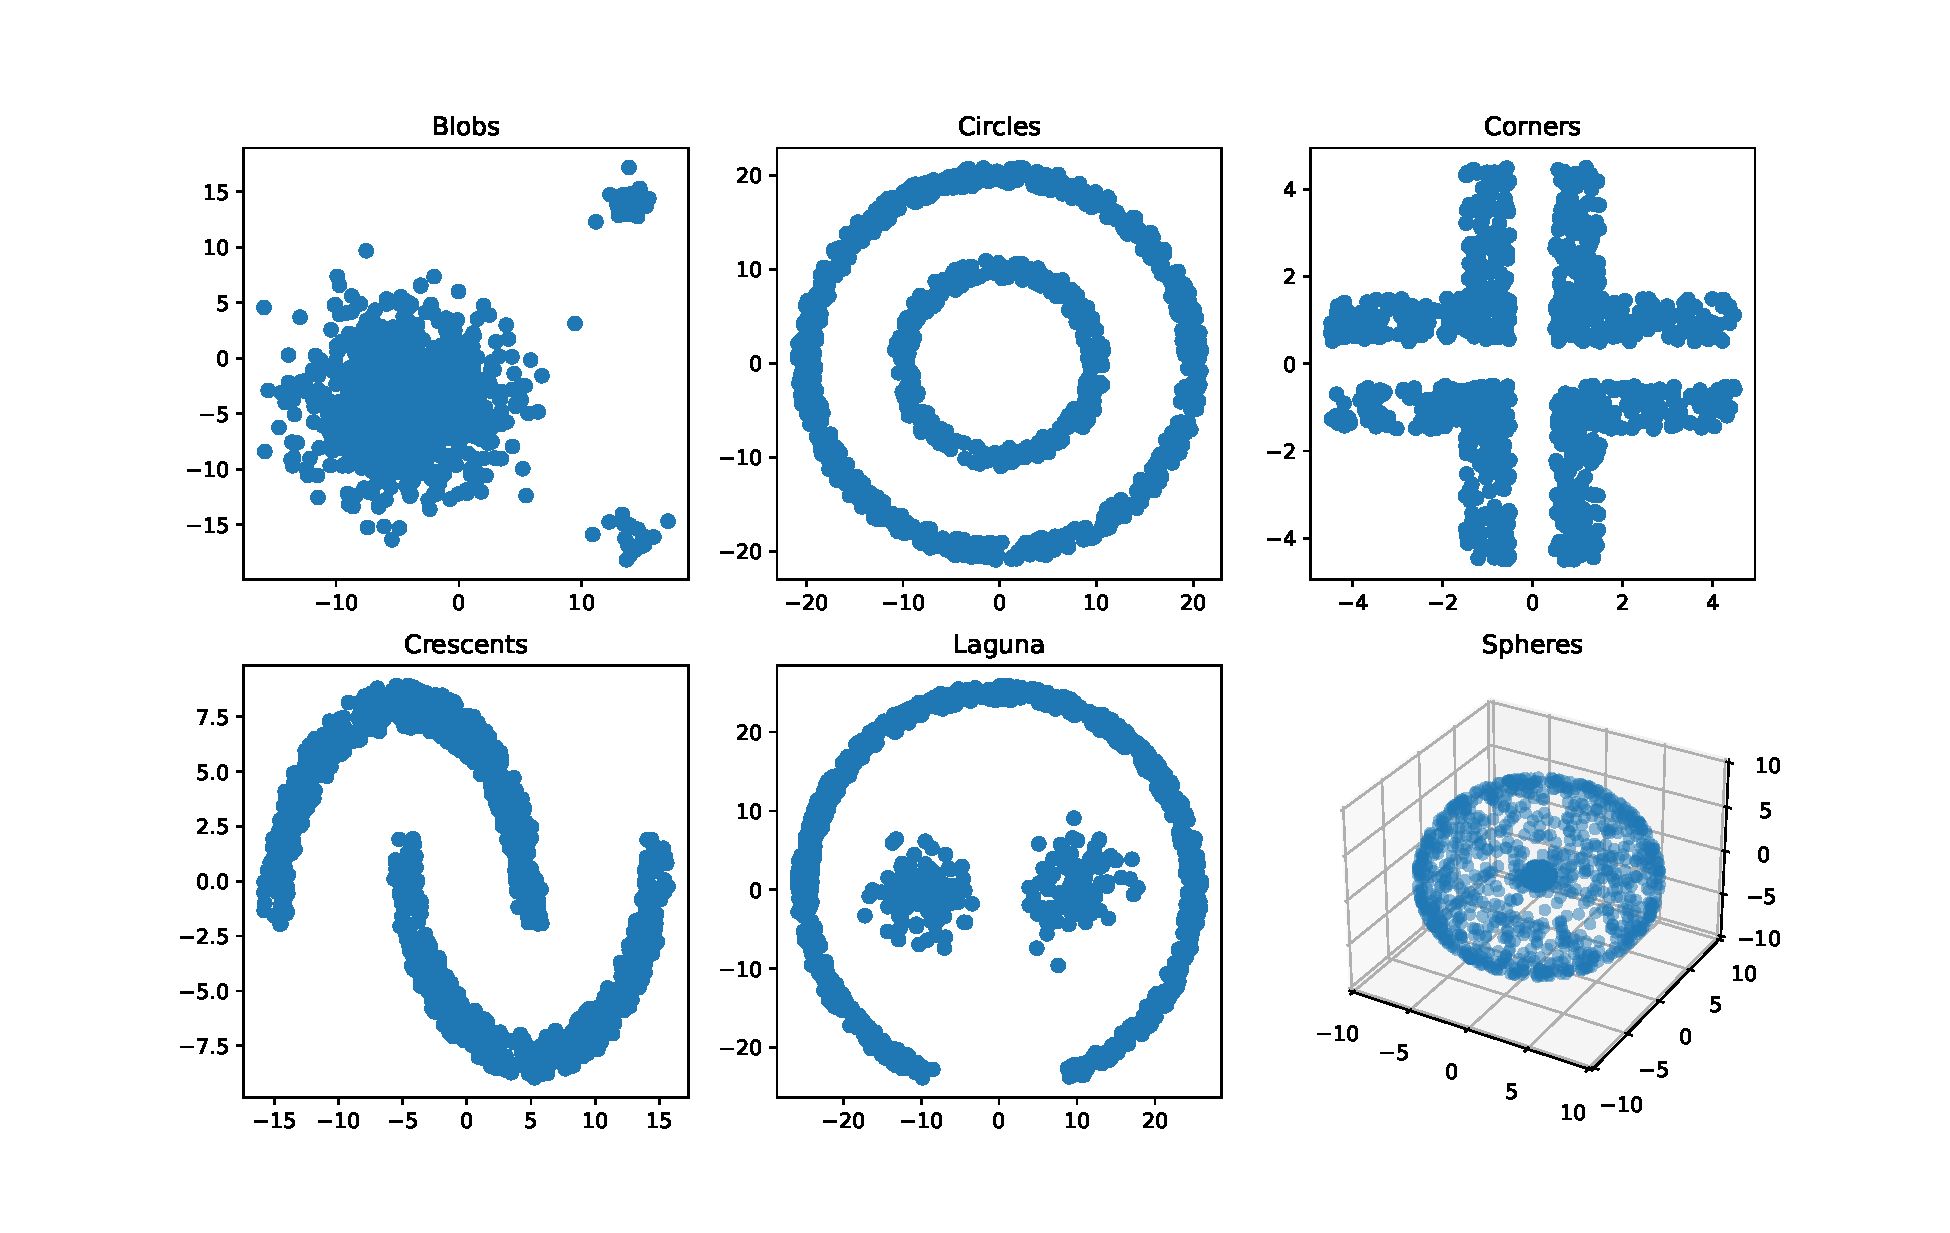
\includegraphics[width=\textwidth]{./data_shapes.pdf}
\caption{Wykresy danych o różnych kształtach z folderu \texttt{dane} o rozmiarze 1000 punktów.}
\label{fig:data-shapes}
\end{figure}

\begin{table}
\centering
\caption{Charakterystyka zbiorów danych dołączonych do projektu.}
\label{id:tab:zbiory}
\begin{tabular}{rrrrrrr}
\toprule
	& \blobs  & \circles & \corners  & \crescents  & \laguna  & \spheres  \\
\midrule
	    liczba klastrów & 3 & 2 & 4 & 2 & 3 & 2 \\
	    liczba wymiarów & 2 & 2 & 2 & 2 & 2 & 3 \\
\bottomrule
\end{tabular}
\end{table}

\begin{figure}
\centering
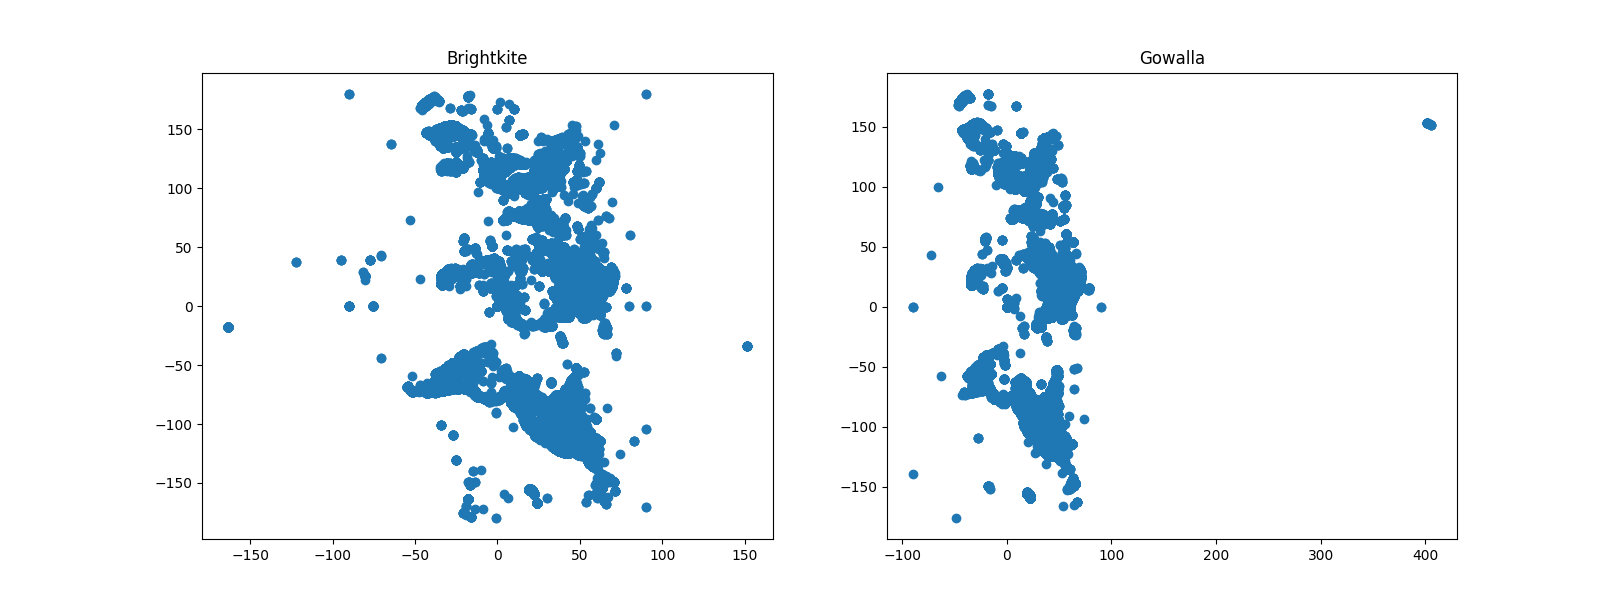
\includegraphics[width=\textwidth]{./gowalla_brightkite_shapes.png}
\caption{Wykresy danych \brightkite i \gowalla.}
\label{fig:gowalla-brightkite-shapes}
\end{figure}

\section{Metodyka badań}

Algorytm \MojAlg{} zbadano pod kątem szybkości wykonania oraz jakości grupowania poprzez porównanie jego efektów z efektami ostrego algorytmu aglomeracyjnego grupowania hierarchicznego \ksremark{konkretnie jakiego?}.

\subsection{Czas grupowania}

Aby znaleźć charakterystykę zależności czasu wykonania algorytmów od ilości danych, przygotowano dane o rozmiarach 500-10000 z krokiem 500.
W tym celu brane były początkowe podzbiory ze zbiorów danych o rozmiarze 10000. Jako że nieistotne były wyniki grupowania, nie było konieczne losowe próbkowanie.

Czas pojedynczego wykonania algorytmu ostrego zmierzono poprzez różnicę czasu rozpoczęcia i zakończenia grupowania hierarchicznego. Wykorzystana została własna implementacja ostrego algorytmu grupowania, analogiczna do wersji rozmytej.
W czasie pojedynczego wykonania algorytmu rozmytego zawarto czas wykonania algorytmu rozmytych $c$-średnich \ksremark{Może warto zapisać nazwę algorytmu do makra? Teraz mamy różny zapis nazwy tego samego algorytmu.}, utworzenia na jego podstawie listy granul oraz rozmytego grupowania hierarchicznego.

Pomiary dla każdego wariantu algorytmu oraz rozmiaru i kształtu danych powtórzono czterokrotnie i obliczono średnią arytmetyczną wyników.

\subsection{Jakość grupowania}

Jakość zmierzono poprzez porówanie wyników algorytmu AgglomerativeClustering \ksremark{$\gets$ trzeba ujednolicić zapis nazwy algorytmu} biblioteki scikit-learn z własną implementacją.

Pomiary wykonano dla wszystkich kształtów i rozmiarów danych. W przypadku algorytmu rozmytego, pomiary przeprowadzono również dla różnych łączności (\SingleLinkage{}, \CompleteLinkage{}), liczebności granul (50, 100, 200), typu relacji liczb rozmytych (trójkątne, wykładnicze, gaussowskie) oraz parametru $\xi \in \{ 0.05, 0.10, 0.15, \ldots, 0.95 \}$.

\subsubsection{Etykietowanie danych}
\label{sec:etykietowanie-danych}

W celu przypisania etykiet do danych z folderu \texttt{dane}, przygotowano pomocniczy skrypt w pliku \texttt{label\_assignment.py}. W zależności od tego, czy dane są dwu- czy trójwymiarowe, przypisanie etykiet odbywa się na inny sposób.

\paragraph{Dane dwuwymiarowe}

Oznaczanie etykiet dla danych dwuwymiarowych wykorzystuje widżet \texttt{LassoSelector} biblioteki \texttt{matplotlib}. Dla każdego pliku z danymi dwuwymiarowymi, wyświetlono wykres połączony z obiektem klasy \texttt{SelectFromCollection} z przykładu \cite{bib:mplt-lasso}. Klasa ta między innymi umożliwia wyznaczenie indeksów i współrzędnych punktów zaznaczonych myszą na wykresie. 

Każdemu punktowi domyślnie przypisano etykietę 0. Po zaznaczeniu zbioru punktów na wykresie, naciśnięcie klawisza cyfry na klawiaturze powoduje przypisanie tym punktom etykiety o danym numerze i wyświetlenie w konsoli informacji, ilu punktom ją przypisano. Proces można powtarzać dowolną ilość razy, można go zakończyć poprzez naciśnięcie klawisza ENTER i zamknięcie wykresu.

W celu ostatecznej weryfikacji pojawia się drugi wykres, na którym każdej etykiecie odpowiada inny kolor. Po zamknięciu tego wykresu, plik z etykietami jest zapisywany w folderze \texttt{dane\_labelled}. Plik ma format zgodny z oryginalnym plikiem z danymi (każdy wiersz to oddzielone znakami tabulacji współrzędne jednego punktu), z dodaną dodatkową kolumną z etykietami punktów.

\paragraph{Dane trójwymiarowe}

W przypadku danych trójwymiarowych skorzystano z faktu, że jedyne dane wykorzystywane w pracy, dla których należy znaleźć etykiety, to dane \spheres{}. Punkty otrzymane z tych danych tworzą dwie sfery: mniejsza, wewnętrzna sfera jest zamknięta w sześcianie o wymiarach $1 \times 1 \times 1$ jednostek, a punkty drugiej, większej sfery znajdują się poza tym sześcianem. Wszystkim punktom, których wszystkie współrzędne mają wartości $\le 1$ przypisano etykietę 1, pozostałym -- 0. Dane z etykietami zostały zapisane w folderze \texttt{dane\_labelled}, w takim samym formacie, jak dane dwuwymiarowe.

\paragraph{Wyniki etykietowania}
\label{sec:wyniki-etykietowania}

Na wykresie \ref{fig:data-shapes-labels} przedstawiono wyniki etykietowania danych. Punkty oznaczone tym samym kolorem posiadają te same etykiety.

W przypadku danych \laguna{} o liczebności 20000 i większej, dwa środkowe klastry przestają być wyraźnie oddzielone od siebie (rys. \ref{fig:laguna20000-labels}). Liczebności tych klastrów po podziale ich narzędziem \texttt{LassoSelector} nie są równe, jak w przypadku mniejszych zbiorów o tym samym kształcie -- różnice wynoszą nie więcej niż 18 punktów. Przy tak dużych zbiorach danych wpływ pojedynczych punktów jest marginalny, należy jednak uwzględnić tę niepewność w analizie wyników jakości grupowania.

\begin{figure}
\centering
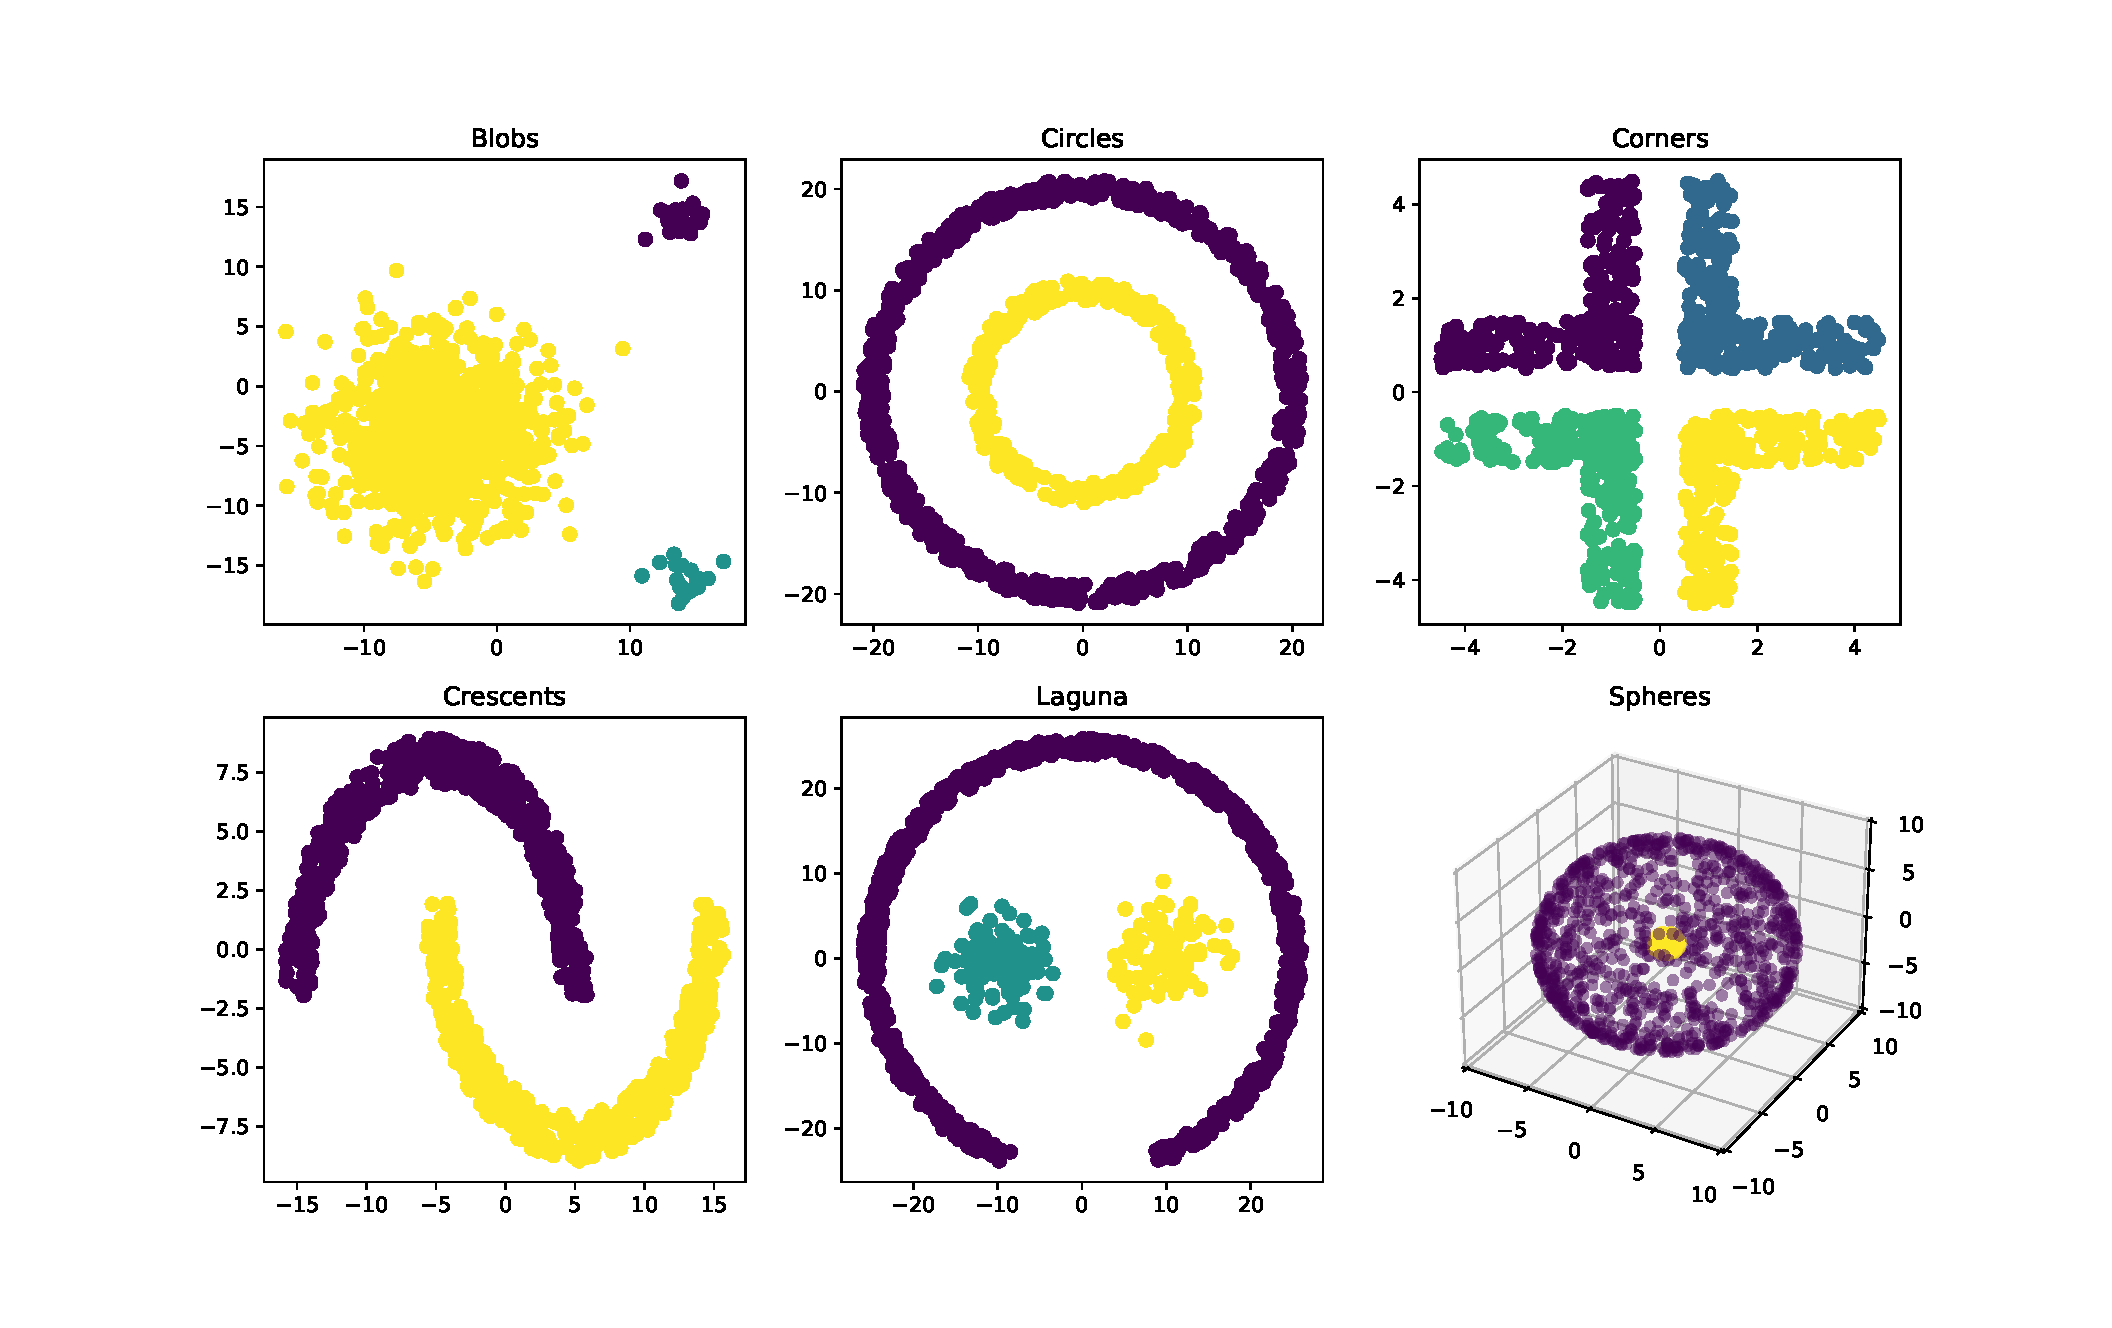
\includegraphics[width=\textwidth]{./data_shapes_labels.pdf}
\caption{Wykresy danych o różnych kształtach z folderu \texttt{dane\_labelled} o rozmiarze 1000 punktów, o etykietach oznaczonych kolorami.}
\label{fig:data-shapes-labels}
\end{figure}

\begin{figure}
\centering
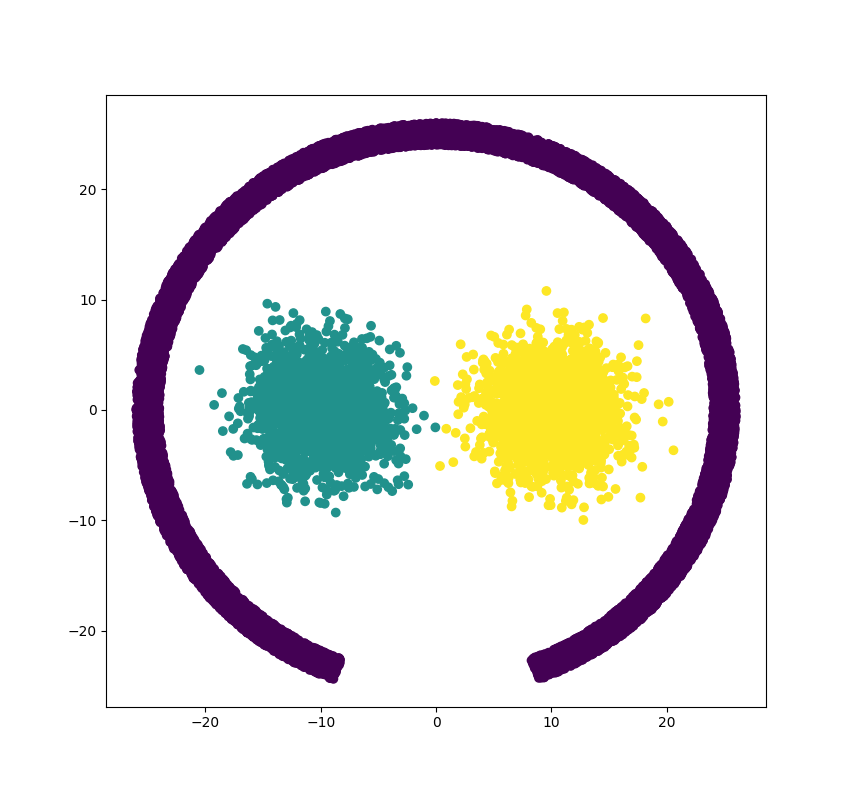
\includegraphics[width=\textwidth]{./laguna20000_labelled.png}
\caption{Wykres danych \laguna{} z folderu \texttt{dane\_labelled} o rozmiarze 20000 punktów, o etykietach oznaczonych kolorami.}
\label{fig:laguna20000-labels}
\end{figure}

\subsubsection{Miara jakości}

\ksremark{Trzeba napisać, na czym polega użyta miara. Opisałbym tę miarę w formie algorytmu. Przyznam się, że z tego opisu nie bardzo bym wiedział, jak to działa.}
Wybranymi miarami jakości grupowania są dokładność, trafność i precyzja.

Rozmyty algorytm grupowania jako wynik zwraca przynależność do klastrów granul, nie oryginalnych danych. Na potrzeby porównania konieczne jest określenie, do której granuli należy każdy punkt. Przynależność tą wyznaczano na dwa sposoby:

\paragraph{Na podstawie macierzy $\mClusterMembership$}

Dla każdego punktu $i$, znajdowana jest granula, dla której wartość odpowiedniego wiersza w macierzy przynależności $\wClusterMembership_i$ jest maksymalna.

\paragraph{Na podstawie relacji $\ast$-podobieństwa $\nPodobienstwo$}

Działanie tej metody przedstawia pseudokod \ref{alg:similarity_membership}.

Dla każdego punktu $i$, przynależność do granuli $j$ obliczana na podstawie wartości operacji $=_\nPodobienstwo$ (wzór \ref{eq:fuzzy-equality}) dla każdego wymiaru punktu i granuli. Operacja ta jest zależna od kształtu granul, dla liczb trójkątnych, wykładniczych i gaussowskich należy wykorzystać odpowiednio wzory \ref{eq:similarity_t}, \ref{eq:similarity_e} lub \ref{eq:similarity_g} uwzględniając, że dla liczby ostrej (współrzędnej oryginalnego punktu) $p = 0$. 

Wyniki dla każdej współrzędnej łączone są t-normą algebraiczną (wzór \ref{eq:algebraic-norms}). Wreszcie określa się, że punkt należy do tej granuli, dla której wynik tego złączenia jest maksymalny.

Należy uwzględnić, że rozszerzalne liczby rozmyte trójkątne posiadają skończony nośnik. Oznacza to, że punkt może nie należeć do żadnej granuli -- dla każdej z nich przynależność będzie zerowa. Punkt taki uznawany jest za szum i nie bierze udziału w wyznaczaniu wartości dokładności, trafności i precyzji, jednak odsetek punktów stanowiących szum jest w tym przypadku dodatkową miarą jakości.

Rysunek \ref{fig:shape-dep} przedstawia przykład takiego przypisania punktów do granul, dla czytelności wykresów wyznaczono jedynie 10 granul. Wykresy dla liczb wykładniczych i gaussowskich są bardzo podobne, ponadto wszystkie punkty są przypisane do granuli. W przypadku liczb trójkątnych, duża część punktów stanowi szum.

\begin{algorithm}[t]
	\caption{Wyznaczenie przynależności punktu do granuli na podstawie relacji $\ast$-podobieństwa $\nPodobienstwo$}
	\label{alg:similarity_membership}
	\begin{algorithmic}[1]
		\Require $\zX$: dane oryginalne
		\Require $\zGranula$: granule wyznaczone przez algorytm \MojAlg{}
		\Require $\wEtykieta_{\Granula}$: wektor o długości $\nGranula$ etykiet wyznaczonych dla wszystkich granul
		\Require $r$: typ relacji (trójkątna, wykładnicza, gaussowska)
		\Procedure{CalculateSimilarityMembership}{$\zX, \zGranula, \wEtykieta, r$}
		\State $\wEtykieta_{\X} \gets []$ \Comment{etykiety punktów}
		\State $szum \gets 0$ \Comment{liczba punktów nieprzynależących do żadnej granuli}
		\For{$\X$ in $\nX$}
		\State $\Etykieta \gets 0$
		\State $\ClusterMembership_{max} \gets 0$
		\For{$i=1$ to $\nGranula$}
		\State $\ClusterMembership \gets (\zGranula[i][1] =_{\nPodobienstwo} \X[1])$
		\For{$j=2$ to liczba wymiarów $\X$}
		\State $\ClusterMembership \gets \ClusterMembership * (\zGranula[i][j] =_{\nPodobienstwo} \X[j])$ \Comment{t-norma algebraiczna}\Comment{\ksremark{Chodzi tutaj o $*$?}}
		\EndFor
		\If{$\ClusterMembership > \ClusterMembership_{max}$}
		\State $\ClusterMembership_{max} \gets \ClusterMembership$
		\State $\Etykieta \gets i$
		\EndIf
		\EndFor
		\If{$\ClusterMembership_{max} > 0$}
		\State dodaj $i$ do $\wEtykieta_{\X}$
		\Else \Comment{punkt nie przynależy do żadnej granuli -- jest szumem}
		\State dodaj $-1$ do $\wEtykieta_{\X}$
		\State $szum \gets szum + 1$
		\EndIf
		\EndFor
		\State \Return $\wEtykieta_{\X}, szum$
		\EndProcedure
	\end{algorithmic}
\end{algorithm}

\begin{figure}
	\centering
	\begin{subfigure}{0.32\textwidth}
		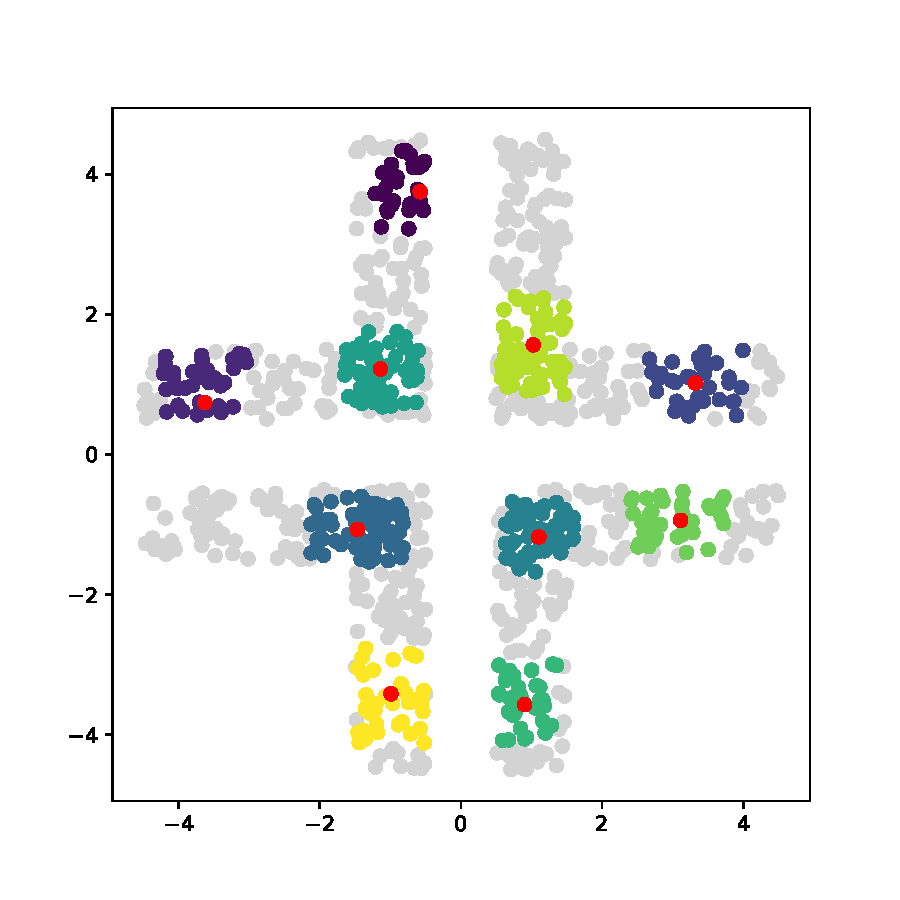
\includegraphics[width=\textwidth]{./shape_dep_t.pdf}
		\caption{Liczby trójkątne}
	\end{subfigure}
	\hfill
	\begin{subfigure}{0.32\textwidth}
		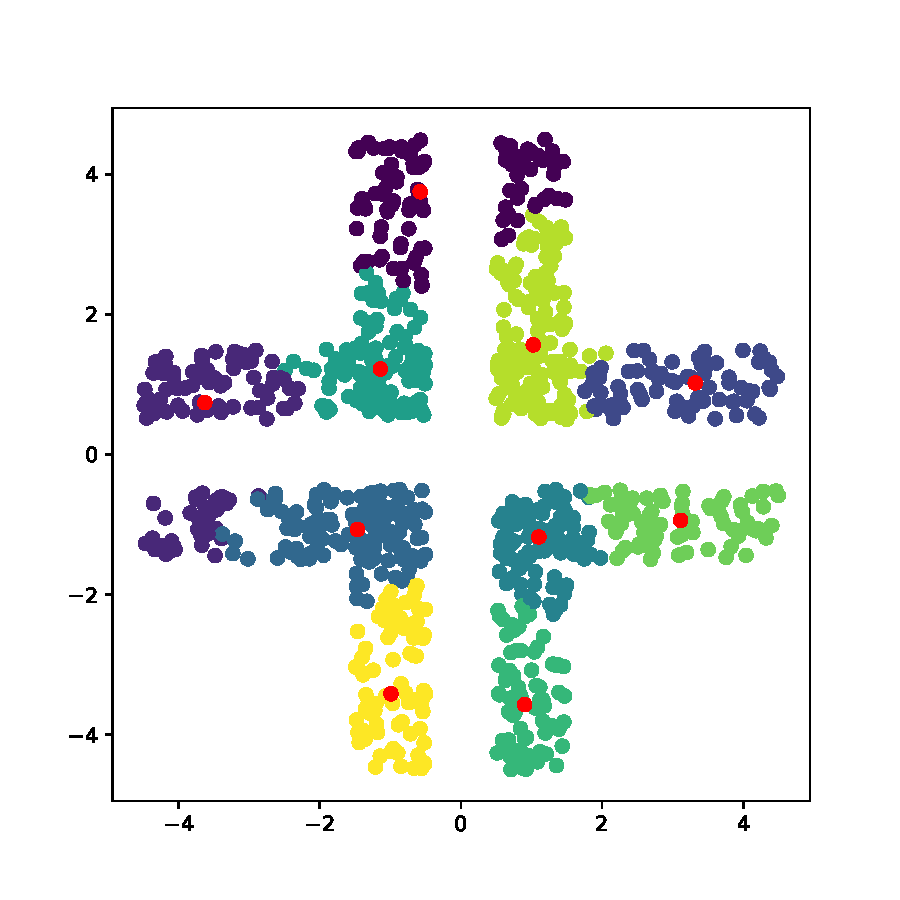
\includegraphics[width=\textwidth]{./shape_dep_e.pdf}
		\caption{Liczby wykładnicze}
	\end{subfigure}
	\hfill
	\begin{subfigure}{0.32\textwidth}
		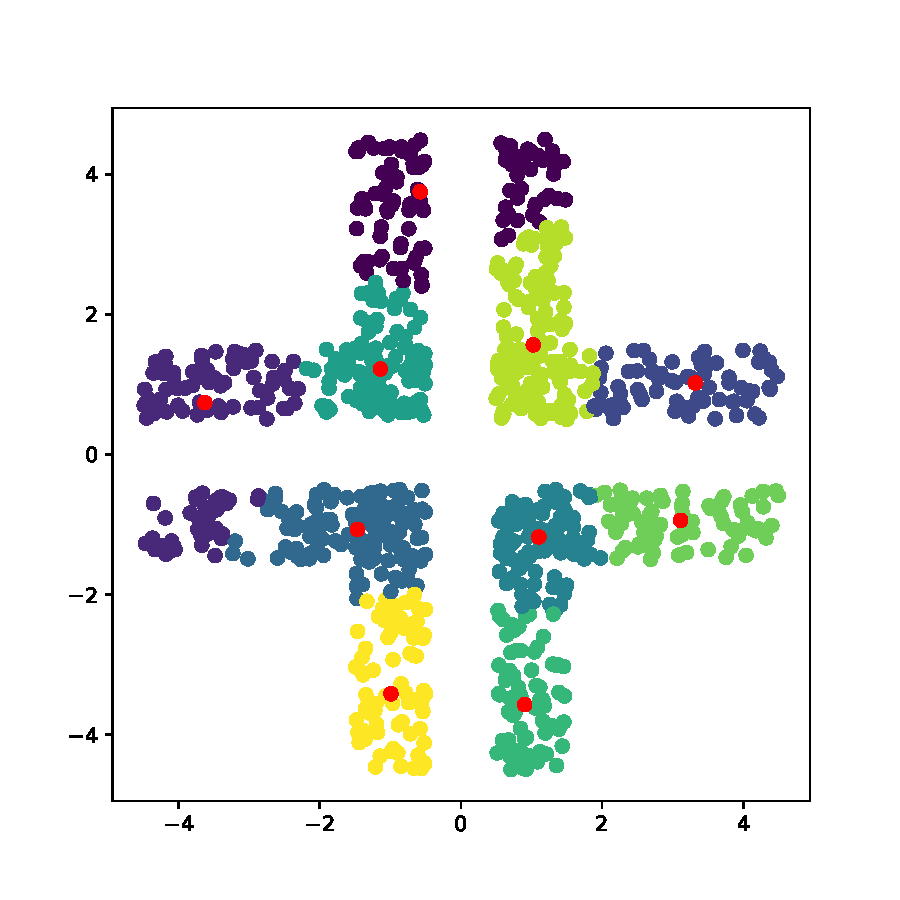
\includegraphics[width=\textwidth]{./shape_dep_g.pdf}
		\caption{Liczby gaussowskie}
	\end{subfigure}
	\caption{Przynależność punktów do granul w zależności od kształtu liczb rozmytych. 10 środków granul oznaczono kolorem czerwonym, punkty należące do różnych granul oznaczone są różnymi kolorami. Kolorem szarym oznaczono punkty stanowiące szum.}
	\label{fig:shape-dep}
\end{figure}

\paragraph{}

\begin{algorithm}[t]
	\caption{Wyznaczenie macierzy $\mConfusionMatrix$}
	\label{alg:calc_l_matrix}
	\begin{algorithmic}[1]
		\Require $\mClusterMembership$: macierz $\nX \times \nX$ przynależności danych do klastrów
		\Require $\wEtykieta_{r}$: wektor o długości $\nX$ etykiet wyznaczonych dla wszystkich punktów przez algorytm ostry
		\Require $\wEtykieta_{g}$: wektor o długości $\nKlaster$ etykiet wyznaczonych dla wszystkich granul przez algorytm \MojAlg
		\Procedure{CalculateLMatrix}{$\mClusterMembership, \wEtykieta_{r}, \wEtykieta_{g}$}
		\State $\mConfusionMatrix \gets$ macierz zerowa $\nKlaster \times \nKlaster$
		\For{$i = 1$ to $\nX$}
		\State $\ClusterMembership \gets$ \Call{argmax}{$\mClusterMembership[i]$} \Comment{Indeks identyfikujący granulę, dla której przynależność punktu $i$-tego jest największa}
		\State inkrementacja $\mConfusionMatrix[\wEtykieta_{r}[i]][\wEtykieta_{g}[\ClusterMembership]]$
		\EndFor
		\State \Return $\mConfusionMatrix$
		\EndProcedure
	\end{algorithmic}
\end{algorithm}

\begin{algorithm}[t]
	\caption{Permutacja macierzy $\mConfusionMatrix$}
	\label{alg:perm_l_matrix}
	\begin{algorithmic}[1]
		\Require $\mConfusionMatrix$: macierz $\nKlaster \times \nKlaster$, wyznaczona przez algorytm \ref{alg:calc_l_matrix}
		\Procedure{PermuteLMatrix}{$\mConfusionMatrix$}
		\For{$i = 1$ to $\nKlaster - 1$}
		\State $(w, k) \gets$ $\arg\max$($\mConfusionMatrix$[i:][i:]) \Comment{Indeksy wiersza i kolumny, w których znajduje się maksymalna wartość podmacierzy $\mConfusionMatrix[i:][i:]$}
		\State $w \gets w + i$
		\State $k \gets k + i$
		\State zamiana kolejnością wiersza $i$-tego i $w$-tego macierzy $\mConfusionMatrix$
		\State zamiana kolejnością kolumny $i$-tej i $k$-tej macierzy $\mConfusionMatrix$
		\EndFor
		\State \Return $\mConfusionMatrix$
		\EndProcedure
	\end{algorithmic}
\end{algorithm}

Wyznaczono macierz $\mConfusionMatrix$, w której wartość elementu $\ConfusionMatrix_{ij}$ jest równa liczbie punktów, dla których oczekiwana etykieta ma wartość $i$ i przynależących do klastra $j$ wyznaczonego przez algorytm \MojAlg{}:
\begin{align}
\ConfusionMatrix_{ij} = \sum_{k=0}^{N} [x_{k} \in i \wedge x_{k} \in j]
\end{align}

Sposób wyznaczenia tej macierzy przedstawiono również na pseudokodzie \ref{alg:calc_l_matrix}.

Numeracja klastrów wyznaczonych przez algorytm \MojAlg{} może być inna od oczekiwanych etykiet ze względu na różną kolejność ich wyznaczenia. Wykorzystując algorytm przedstawiony na pseudokodzie \ref{alg:perm_l_matrix}, wyznaczono taką permutację wierszy i kolumn macierzy $\mConfusionMatrix$, która maksymalizuje wartości na przekątnej. 

Z uzyskanej w ten sposób macierzy pomyłek, dokładność wyznaczana jest jako suma wartości na przekątnej macierzy podzielona przez całkowitą liczbę danych:
\begin{align}
\accuracy = \frac{\sum_{i=0}^{\nKlaster}\ConfusionMatrix_{ii}}{N}
\end{align}
lub
\begin{align}
\accuracy = \frac{\sum_{i=0}^{\nKlaster}\ConfusionMatrix_{ii}}{\sum_{i=0}^{\nKlaster}\sum_{j=0}^{\nKlaster}\ConfusionMatrix_{ij}},
\end{align}
gdzie $\nKlaster$ to liczba klastrów.

Trafność ($\recall$) i precyzja ($\precision$) wyznaczane są najpierw osobno dla każdego klastra $\klaster$:
%
\begin{align}
	\recall_{\klaster} = \frac{\ConfusionMatrix_{\klaster\klaster}}{\sum_{i=0}^{\nKlaster}\ConfusionMatrix_{\klaster i}},
\end{align}
%
\begin{align}
	\precision_{\klaster} = \frac{\ConfusionMatrix_{\klaster\klaster}}{\sum_{i=0}^{\nKlaster}\ConfusionMatrix_{i \klaster}}.
\end{align}
%
Trafność i precyzja dla całości wyników otrzymywane są jako średnia arytmetyczna metryk częściowych:
\begin{align}
	\recall = \frac{\sum_{i=0}^{\nKlaster}\recall_{i}}{\nKlaster},
\end{align}
\begin{align}
	\precision = \frac{\sum_{i=0}^{\nKlaster}\precision_{i}}{\nKlaster}.
\end{align}
%
Tak obliczona średnia oznacza, że każdy klaster ma jednakową wagę dla ostatecznego wyniku. Trafność i precyzja będą więc bardziej niż dokładność czułe na błędy przy klasyfikacji danych dla klastrów o różnej docelowej liczności. 

Sposób obliczenia metryk jakości przedstawia również pseudokod \ref{alg:calc_quality}.

\begin{algorithm}[t]
	\caption{Wyznaczenie dokładności, trafności i precyzji}
	\label{alg:calc_quality}
	\begin{algorithmic}[1]
		\Require $\mConfusionMatrix$: macierz $\nKlaster \times \nKlaster$, otrzymana na podstawie algorytmu \ref{alg:perm_l_matrix}
		\Require $\nX$: liczba danych
		\Procedure{CalculateQualityMetrics}{$\mConfusionMatrix, \nX$}
		\State $diag \gets 0$ \Comment{Suma wartości na przekątnej macierzy $\mConfusionMatrix$}
		\State $\recall \gets 0$
		\State $\precision \gets 0$
		\State $mian\_\recall \gets $ sumy wartości dla każdego wiersza macierzy $\mConfusionMatrix$
		\State $mian\_\precision \gets $ sumy wartości dla każdej kolumny macierzy $\mConfusionMatrix$
		\For{$i = 1$ to $\nKlaster$}
		\State $diag \gets diag + \mConfusionMatrix[i, i]$
		\If {$mian\_\recall[i] > 0 $}
			\State $\recall \gets \recall + \mConfusionMatrix[i, i] / mian\_\recall[i]$
		\EndIf
		\If {$mian\_\precision[i] > 0 $}
			\State $\precision \gets \precision + \mConfusionMatrix[i, i] / mian\_\precision[i]$
		\EndIf
		\EndFor
		\State $\accuracy \gets diag / \nX$
		\State $\recall \gets \recall / \nKlaster$
		\State $\precision \gets \precision / \nKlaster$
		\State \Return $\accuracy, \recall, \precision$
		\EndProcedure
	\end{algorithmic}
\end{algorithm}

\section{Wyniki}

\subsection{Czas grupowania}

Algorytm \MojAlg{}, który wykorzystuje wstępną granulację FCM, ma znacząco mniejszy czas wykonania w stosunku do algorytmu ostrego.
Charakterystykę czasu wykonania algorytmów w zależności od liczby danych przedstawiono na rys. \ref{fig:circles-times}.

\begin{figure}
\centering
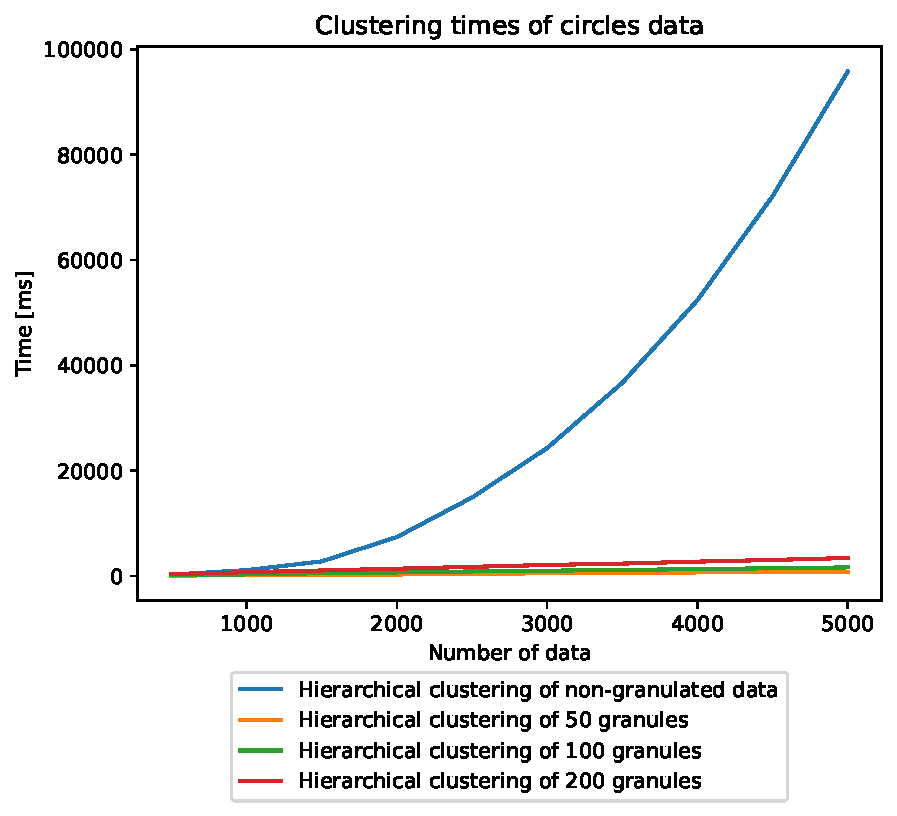
\includegraphics{./circles_times.pdf}
\caption{Charakterystyka czasu wykonania algorytmów ostrego i rozmytego dla różnej liczby granul od liczby danych wejściowych (circles).}
\label{fig:circles-times}
\end{figure}
\ksremark{Rys. \ref{fig:circles-times}: Opis wykresów musi być po polsku.}


Dla obydwu algorytmów, złożoność czasowa grupowania hierarchicznego wynosi $O(n^{3})$, jednak w przypadku algorytmu rozmytego dotyczy ona tylko granul, których liczba jest stała.
Złożoność czasowa algorytmu rozmytych $c$-średnich wynosi $O(n)$, więc jest on mniej wrażliwy na zwiększanie rozmiaru danych wejściowych. \ksremark{To napiszemy w rozdziale 3.}

\ksremark{Jak jakość grupowania zależy do liczby granul?}

\subsection{Jakość grupowania}

Na wykresach wyników grupowania hierarchicznego metodą rozmytą punkty szare odpowiadają współrzędnym oryginalnych danych. Wyjątkiem są wykresy danych \spheres, gdzie oryginalne punkty pominięto, aby zachować czytelność wykresu. Punkty kolorowe odpowiadają środkom granul, gdzie środki o tym samym kolorze należą do tego samego klastra. 
Elipsy (elipsoidy dla \spheres) w kolorze magenta wizualizują rozmycie granul, gdzie długość każdej półosi jest równa dwukrotności rozmycia w danym wymiarze. Mnożnik ten został wybrany ze względu na dobrą czytelność wynikowych wykresów.

\subsubsection{Dane generowane}

\paragraph{Zależność od kształtu danych}

Dokładność grupowania danych w zależności od ich kształtu dla łączności \SingleLinkage{} i \CompleteLinkage{} przedstawiono w tabeli \ref{id:tab:acc-ksztalt}, trafność -- w tabeli \ref{id:tab:rec-ksztalt}, a precyzję -- w tabeli \ref{id:tab:prec-ksztalt}.

W przypadku \SingleLinkage{}, najlepszą dokładność, trafność i precyzję zaobserwowano dla danych \crescents. Dane \corners\ mają najgorszą dokładność, a dane \blobs\ -- najgorszą trafność i precyzję. Wyniki przeanalizowano również na podstawie wykresów.


\begin{table}
\centering
\caption{Dokładność grupowania hierarchicznego danych w zależności od ich kształtu i wykorzystanej łączności}
\label{id:tab:acc-ksztalt}
\begin{tabular}{lcc}
\toprule
            & \multicolumn{2}{c}{dokładność}\\
            \cmidrule{2-3}
	kształt & \SingleLinkage{} &  \CompleteLinkage{} \\
\midrule
	    \blobs\  & 98,6881\% & 87,1617\% \\
		\circles\ & 99,7621\% & 56,8455\% \\
		\corners\  & 94,5375\% & 50,9458\% \\
		\crescents\  & 99,9536\% & 95,7456\% \\
		\laguna\  & 98,8489\% & 46,1161\% \\
		\spheres\  & 98,6634\% & 71,0699\% \\
\bottomrule
\end{tabular}
\end{table}  
\ksremark{Tab. \ref{id:tab:acc-ksztalt}: `Dokładność' to ta miara z macierzą, prawda?}
\ksremark{Tab. \ref{id:tab:acc-ksztalt}: Mamy jedno wykonanie algorytmu?}
\ksremark{Jak się zmienia dokładność w zależności od liczby granul?}

\begin{table}
\centering
\caption{Trafność grupowania hierarchicznego danych w zależności od ich kształtu i wykorzystanej łączności}
\label{id:tab:rec-ksztalt}
\begin{tabular}{rrr}
\toprule
	kształt & trafność \SingleLinkage{} & trafność \CompleteLinkage{} \\
\midrule
	    \blobs\  & 87,9054\% & 89,5804\% \\
		\circles\ & 99,6294\% & 49,7170\% \\
		\corners\  & 94,5375\% & 50,9458\% \\
		\crescents\  & 99,9536\% & 95,7456\% \\
		\laguna\  & 97,2418\% & 54,6761\% \\
		\spheres\  & 94,6116\% & 40,3605\% \\
\bottomrule
\end{tabular}
\end{table}  

\begin{table}
\centering
\caption{Precyzja grupowania hierarchicznego danych w zależności od ich kształtu i wykorzystanej łączności}
\label{id:tab:prec-ksztalt}
\begin{tabular}{rrr}
\toprule
	kształt & precyzja \SingleLinkage{} & precyzja \CompleteLinkage{} \\
\midrule
	    \blobs\  & 86,6801\% & 81,8197\% \\
		\circles\ & 99,7763\% & 49,5504\% \\
		\corners\  & 94,8456\% & 47,4230\% \\
		\crescents\  & 99,9711\% & 96,6097\% \\
		\laguna\  & 97,6756\% & 39,5390\% \\
		\spheres\  & 94,2357\% & 44,1444\% \\
\bottomrule
\end{tabular}
\end{table}  

Wykresy wyników grupowania danych \blobs\  (rys. \ref{fig:blobs1000e}) pokazują, że wysoka dokładność uzyskana dla nich z macierzy pomyłek nie przekłada się na zgodność wyników z oczekiwaniami.
Ze względu na dużą dysproporcję danych pomiędzy trzema klastrami (48:1:1), algorytm fuzzy C-means często traktuje dwa mniejsze z nich jako szum i nie tworzy dla nich granul.
Zawierają one jednak jedynie 4\% danych, dlatego dokładność grupowania pozostaje wysoka. 
Trafność i precyzja lepiej odzwierciedlają zgodność z oczekiwaniami -- są znacznie niższe od dokładności. Mniejsze klastry mają tę samą wagę, co większy klaster, dlatego niepoprawne grupowania wyraźnie wpływają na wartość metryki.

Dane \circles\ (rys. \ref{fig:circles20000g}) mają drugie najwyższe wyniki dokładności, trafności i precyzji. Dla mniejszej liczby (50) rozmyte odległości między granulami położonymi na zewnętrznym okręgu są większe niż między okręgiem zewnętrznym a wewnętrznym, jedyne błędy grupowania pojawiają się dla tej liczebności granul, dla wysokich wartości parametru $\xi$ ($0.9, 0.95$). Okrąg zewnętrzny jest też bardziej liczny niż wewnętrzny (proporcja 7:3). Dysproporcja ta nie jest jednak tak duża, jak w przypadku \blobs\, algorytm rozmytych $c$-średnich tworzy granule w równomiernych odstępach.

Klastry dla danych \corners\  mają nierównomierną gęstość, przez co algorytm rozmytych $c$-średnich tworzy więcej granul bliżej środka układu współrzędnych (rys. \ref{fig:corners1000e}).
Odległości między granulami położonymi na ,,ramionach'' i w ,,środkach'' klastrów są na tyle duże, że odległości ,,środków'' różnych klastrów mogą być od nich mniejsze.
Wszystkie klastry mają tę samą liczebność, wartości dokładności, trafności i precyzji są zbliżone do siebie.

Dane \crescents\  tworzą dwa klastry o identycznej liczebności i gęstości, dzięki czemu dokładność, trafność i precyzja ich grupowania są najlepsze (rys. \ref{fig:crescents1000t}). Ze względu na bliskie położenie końców łuków, przy dużym rozmyciu wciąż możliwe są błędy, jednak szansa na nie jest bardzo mała. Dla 1368 kombinacji parametrów, dla których przeprowadzono pomiary, błędy pojawiły się w 3 przypadkach: przy 50 granulach o kształcie wykładniczym, parametrze $\xi=0.95$, dla liczebności danych wejściowych 20000, 40000 i 50000.

Dla danych \laguna\, błędy mogą pojawić się, gdy pojedyncze granule utworzone zostają w większej odległości od środkowego klastra, do którego oczekiwane jest, że powinny należeć. Punkt taki może wtedy zostać zakwalifikowany, jako osobny klaster, co na rysunku \ref{fig:laguna2000g} pokazują przykłady dla 50 granul i $\xi={0.5, 0.9}$ oraz 200 granul i $\xi=0.9$. Podobny błąd przedstawia wykres dla 200 granul i $\xi=0.5$ -- pewna grupa punktów na otaczającym okręgu jest na tyle oddalona od pozostałych, że zostaje uznana za osobny klaster, dwa klastry środkowe są łączone. Powyżej liczebności 20000 punktów włącznie, dokładność nigdy nie osiąga 100\%, jednak najczęściej wynosi powyżej 99.9\%. Jak zaznaczono w sekcji dotyczącej etykietowania danych (sekcja \ref{sec:wyniki-etykietowania}), środkowe klastry są na tyle zbliżone do siebie, że na podstawie wykresu nie można definitywnie określić, które punkty pomiędzy nimi należą do którego z nich. Pojedyncze punkty mogą więc być klasyfikowane niepoprawnie z punktu widzenia przypisanych do nich etykiet. Proporcja danych wynosi 8:1:1 (otaczający okrąg ma większą liczebność), jednak jakość grupowania jest na tyle wysoka, że zarówno dokładność, jak i trafność i precyzja mają podobne wartości.

W przypadku danych \spheres\  (rys. \ref{fig:spheres1000e}) można zauważyć, że wyniki poprawiają się wraz ze zwiększeniem liczby granul i zmniejszeniem wartości parametru $\xi$. Proporcja liczebności klastrów wynosi 9:1, trafność i precyzja są o około 4 punkty procentowe mniejsze od dokładności.

\begin{figure}
\centering
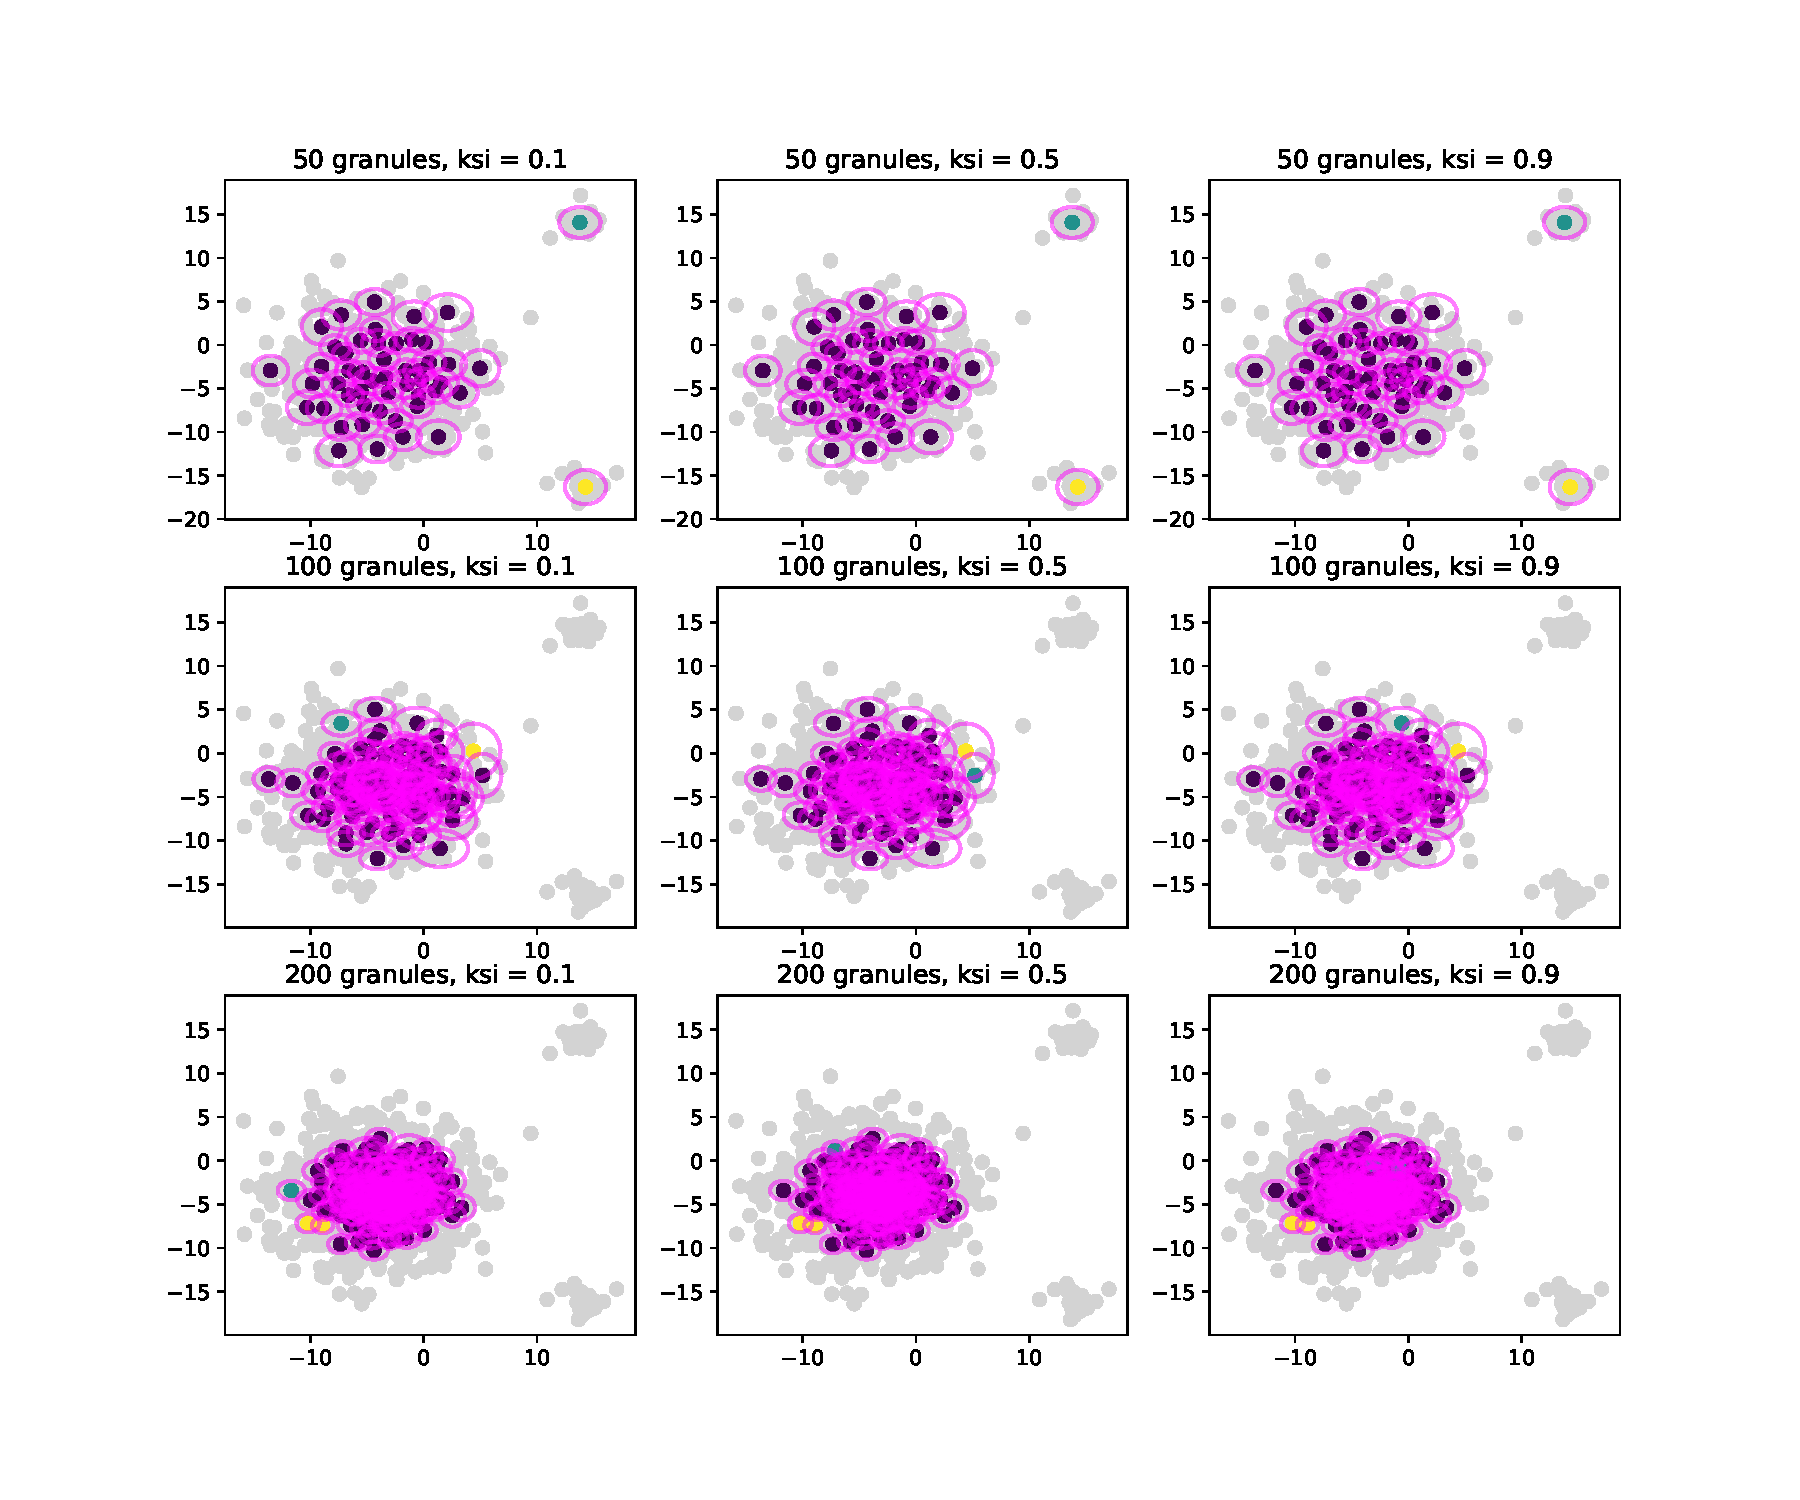
\includegraphics[width=\textwidth]{./blobs1000e.pdf}
\caption{Efekty wykonania grupowania \MojAlg\ dla danych \blobs\  o~rozmiarze 1000 i wykładniczej relacji między liczbami rozmytymi, przy łączności \SingleLinkage{}.}
\label{fig:blobs1000e}
\end{figure}

\begin{figure}
\centering
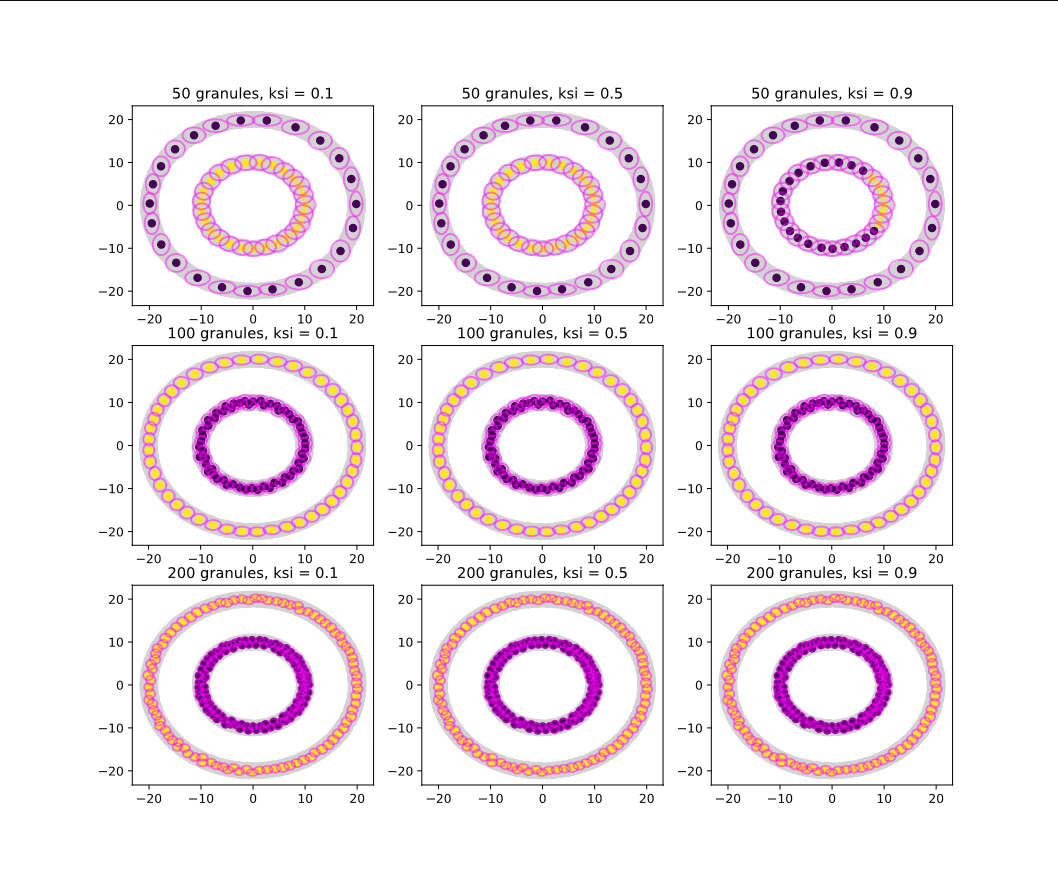
\includegraphics[width=\textwidth]{./circles20000g.png}
\caption{Efekty wykonania grupowania \MojAlg\ dla danych \circles\ o rozmiarze 20000 i gaussowskiej relacji między liczbami rozmytymi, przy łączności \SingleLinkage{}.}
\label{fig:circles20000g}
\end{figure}

\begin{figure}
\centering
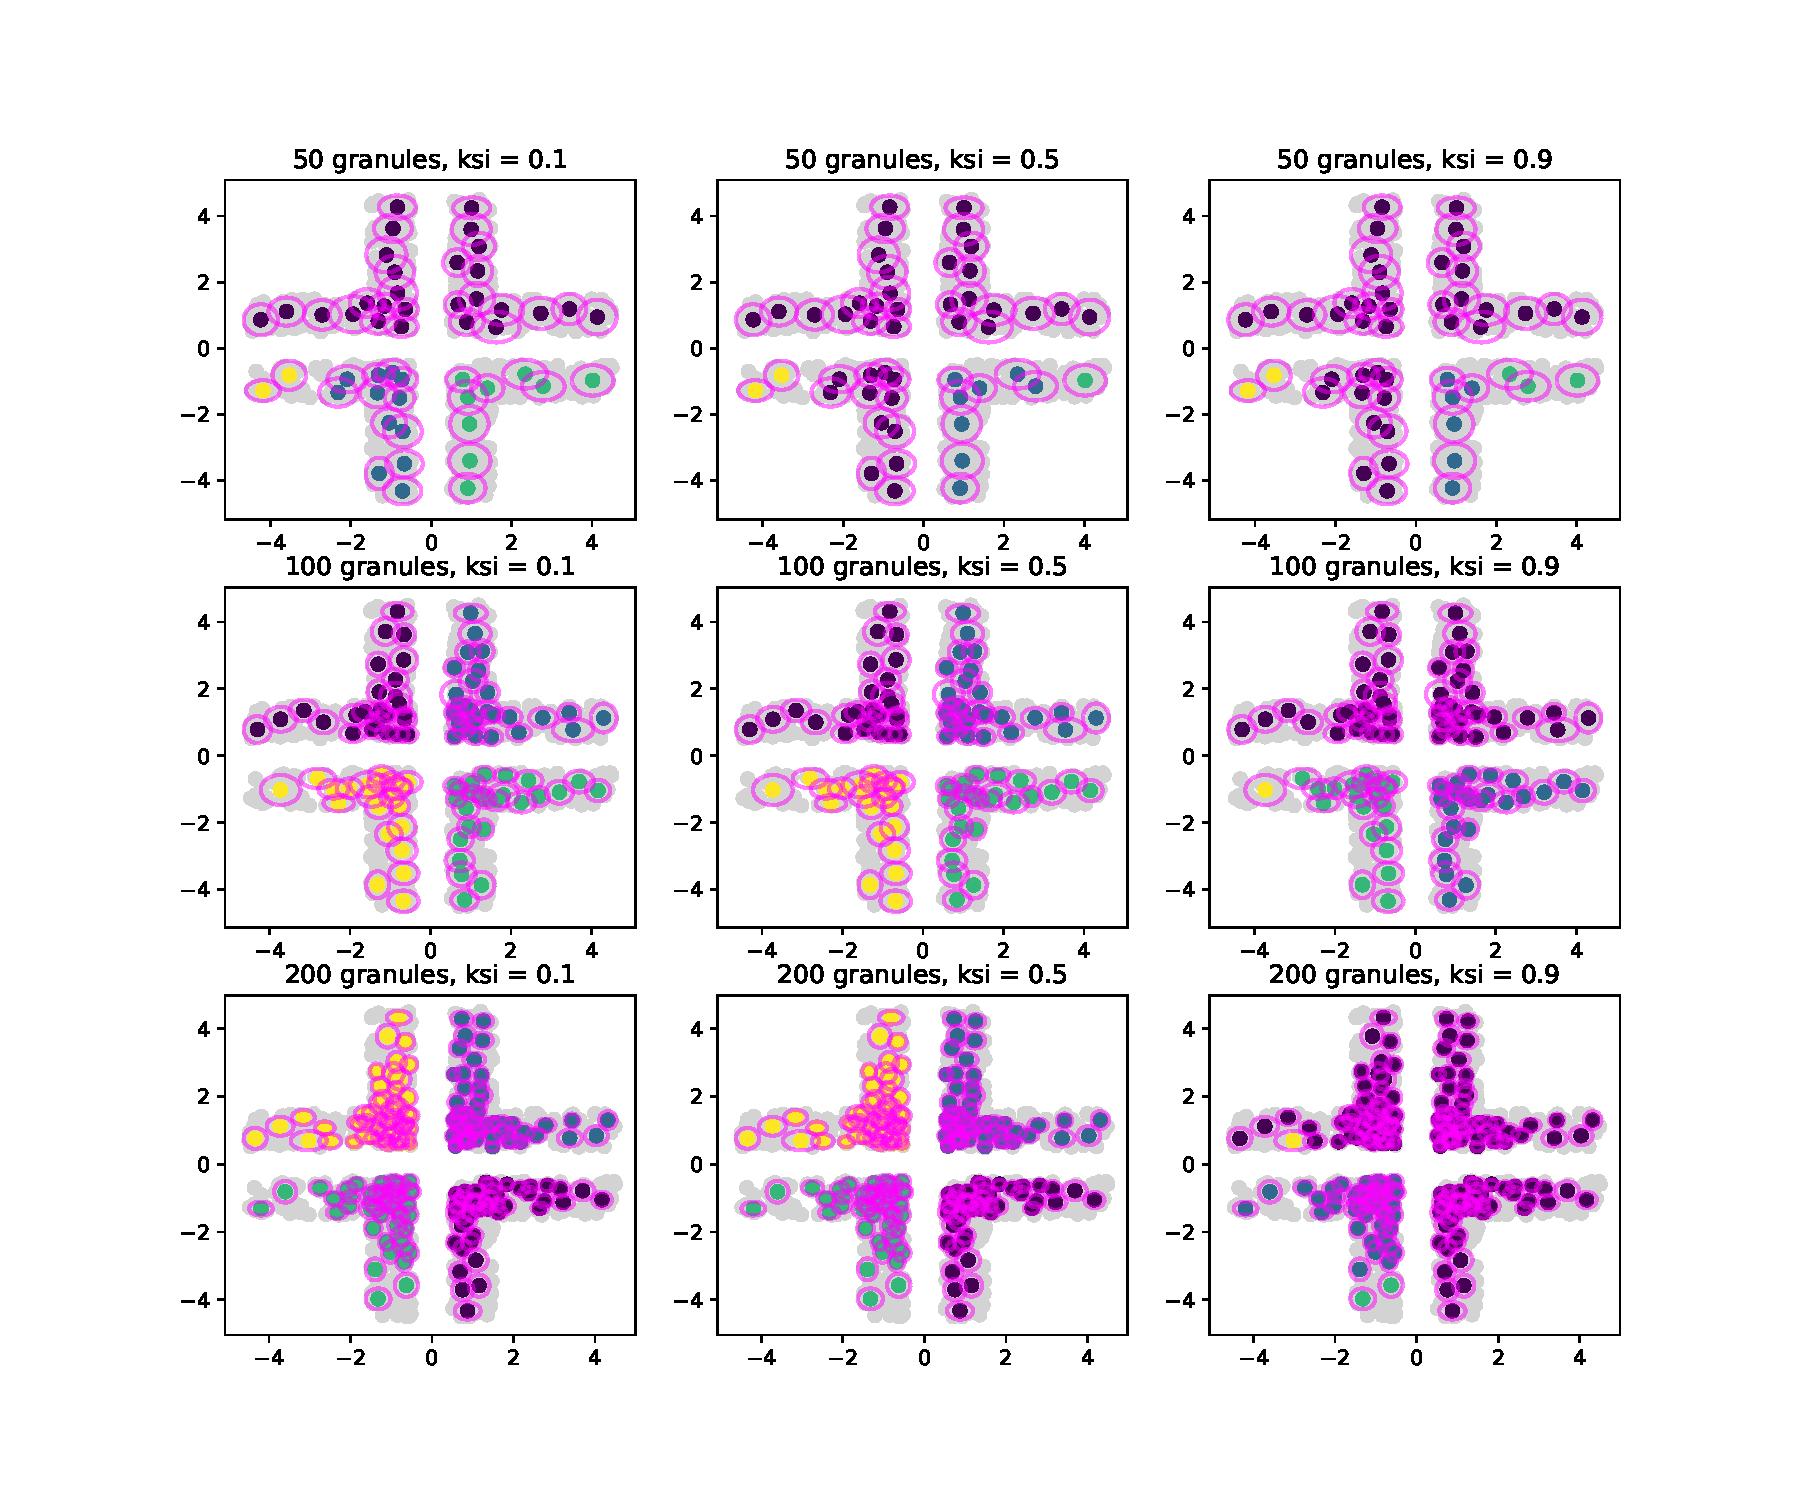
\includegraphics[width=\textwidth]{./corners1000e.pdf}
\caption{Efekty wykonania grupowania \MojAlg\ dla danych \corners\  o rozmiarze 1000 i wykładniczej relacji między liczbami rozmytymi, przy łączności \SingleLinkage{}.}
\label{fig:corners1000e}
\end{figure}

\begin{figure}
\centering
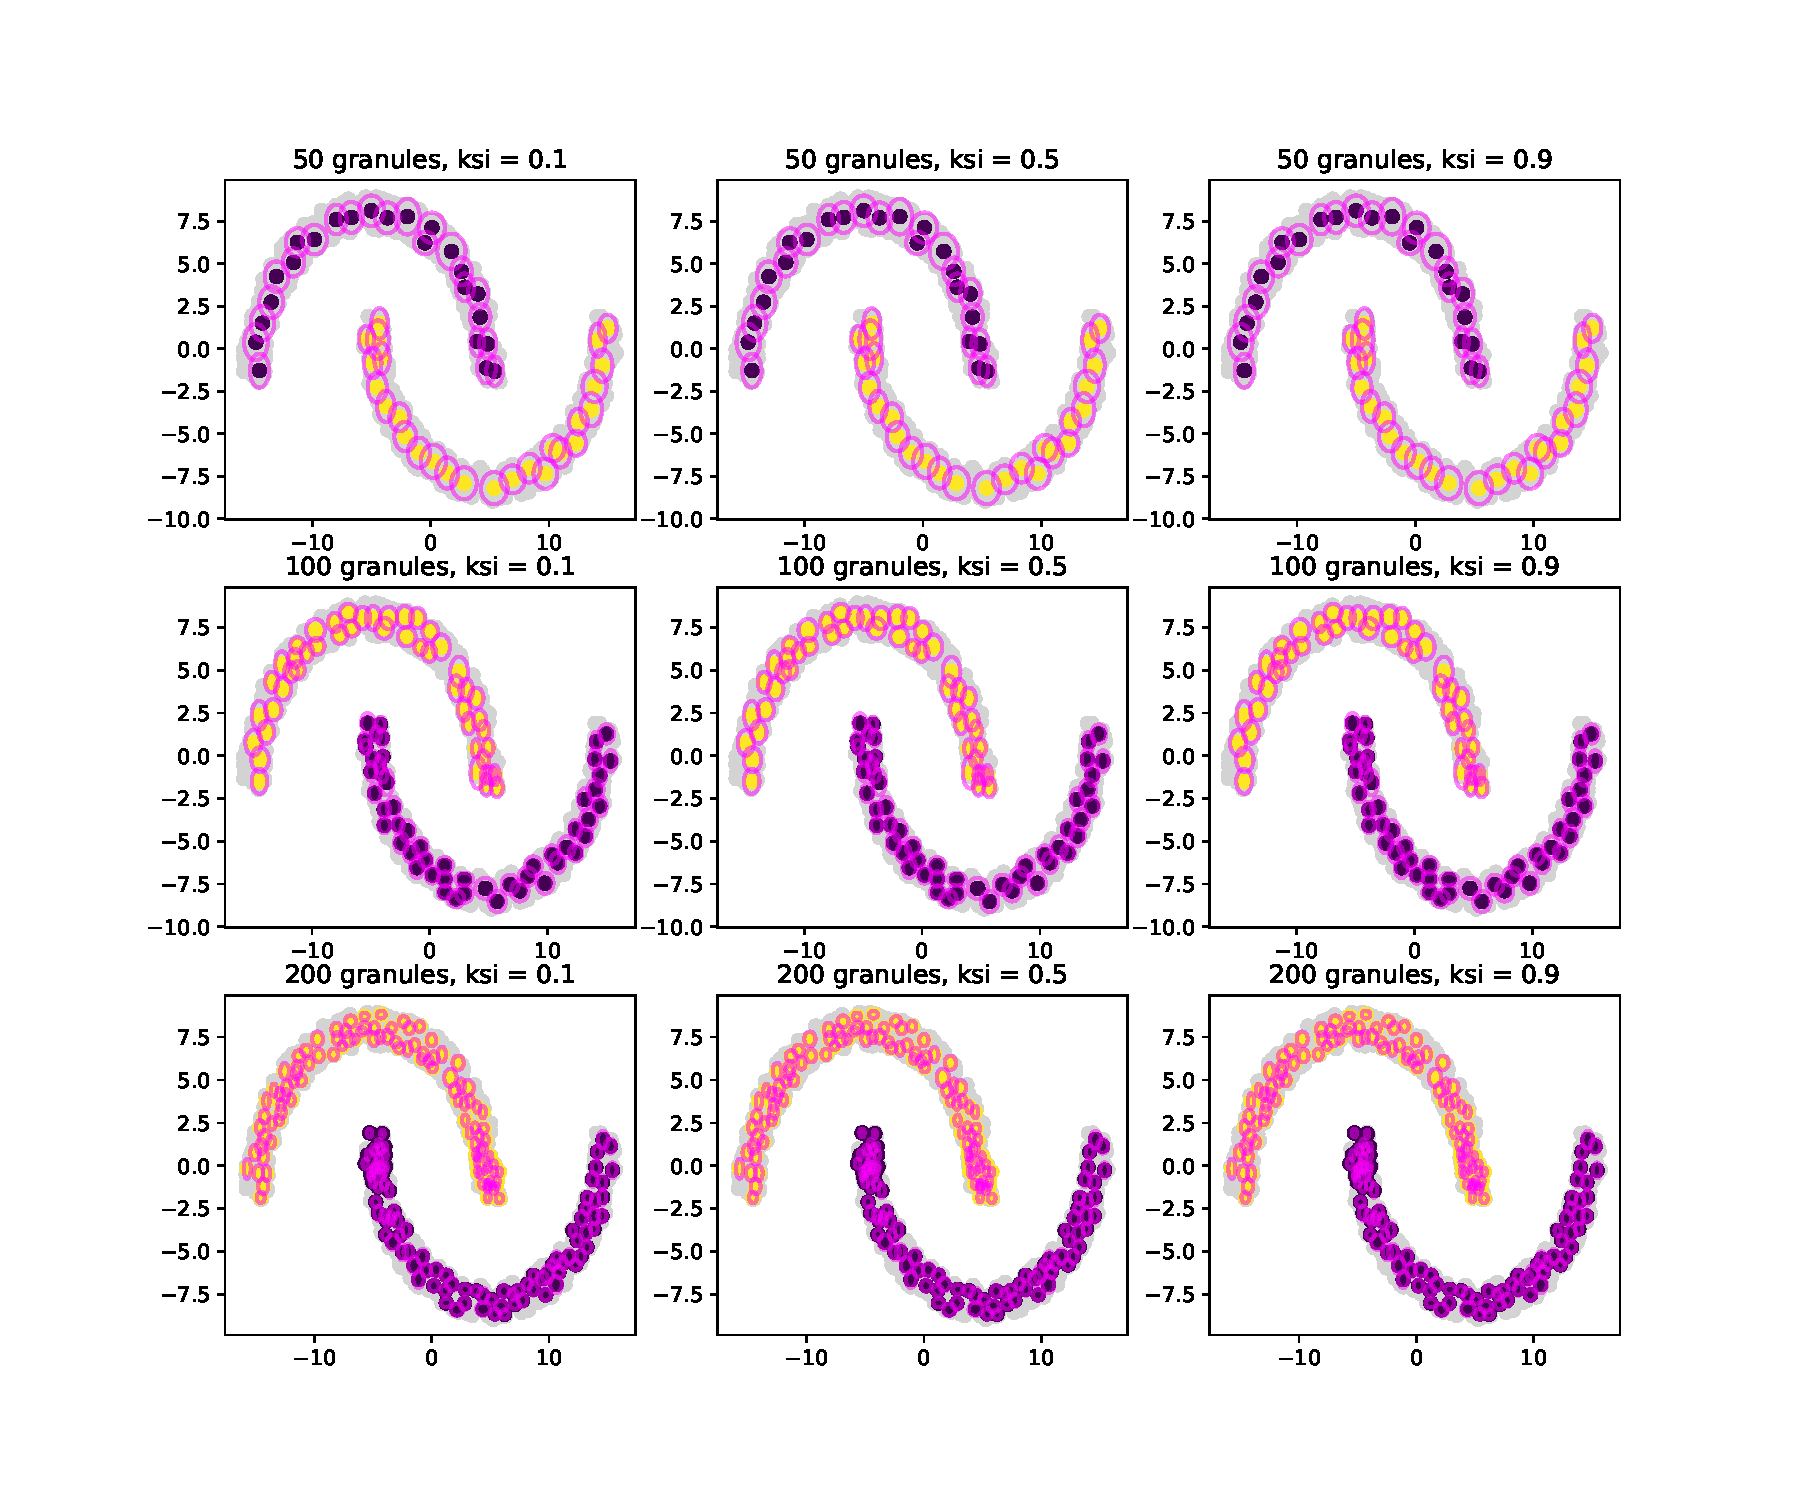
\includegraphics[width=\textwidth]{./crescents1000t.pdf}
\caption{Efekty wykonania grupowania \MojAlg\ dla danych \crescents\  o rozmiarze 1000 i trójkątnej relacji między liczbami rozmytymi, przy łączności \SingleLinkage{}.}
\label{fig:crescents1000t}
\end{figure}

\begin{figure}
\centering
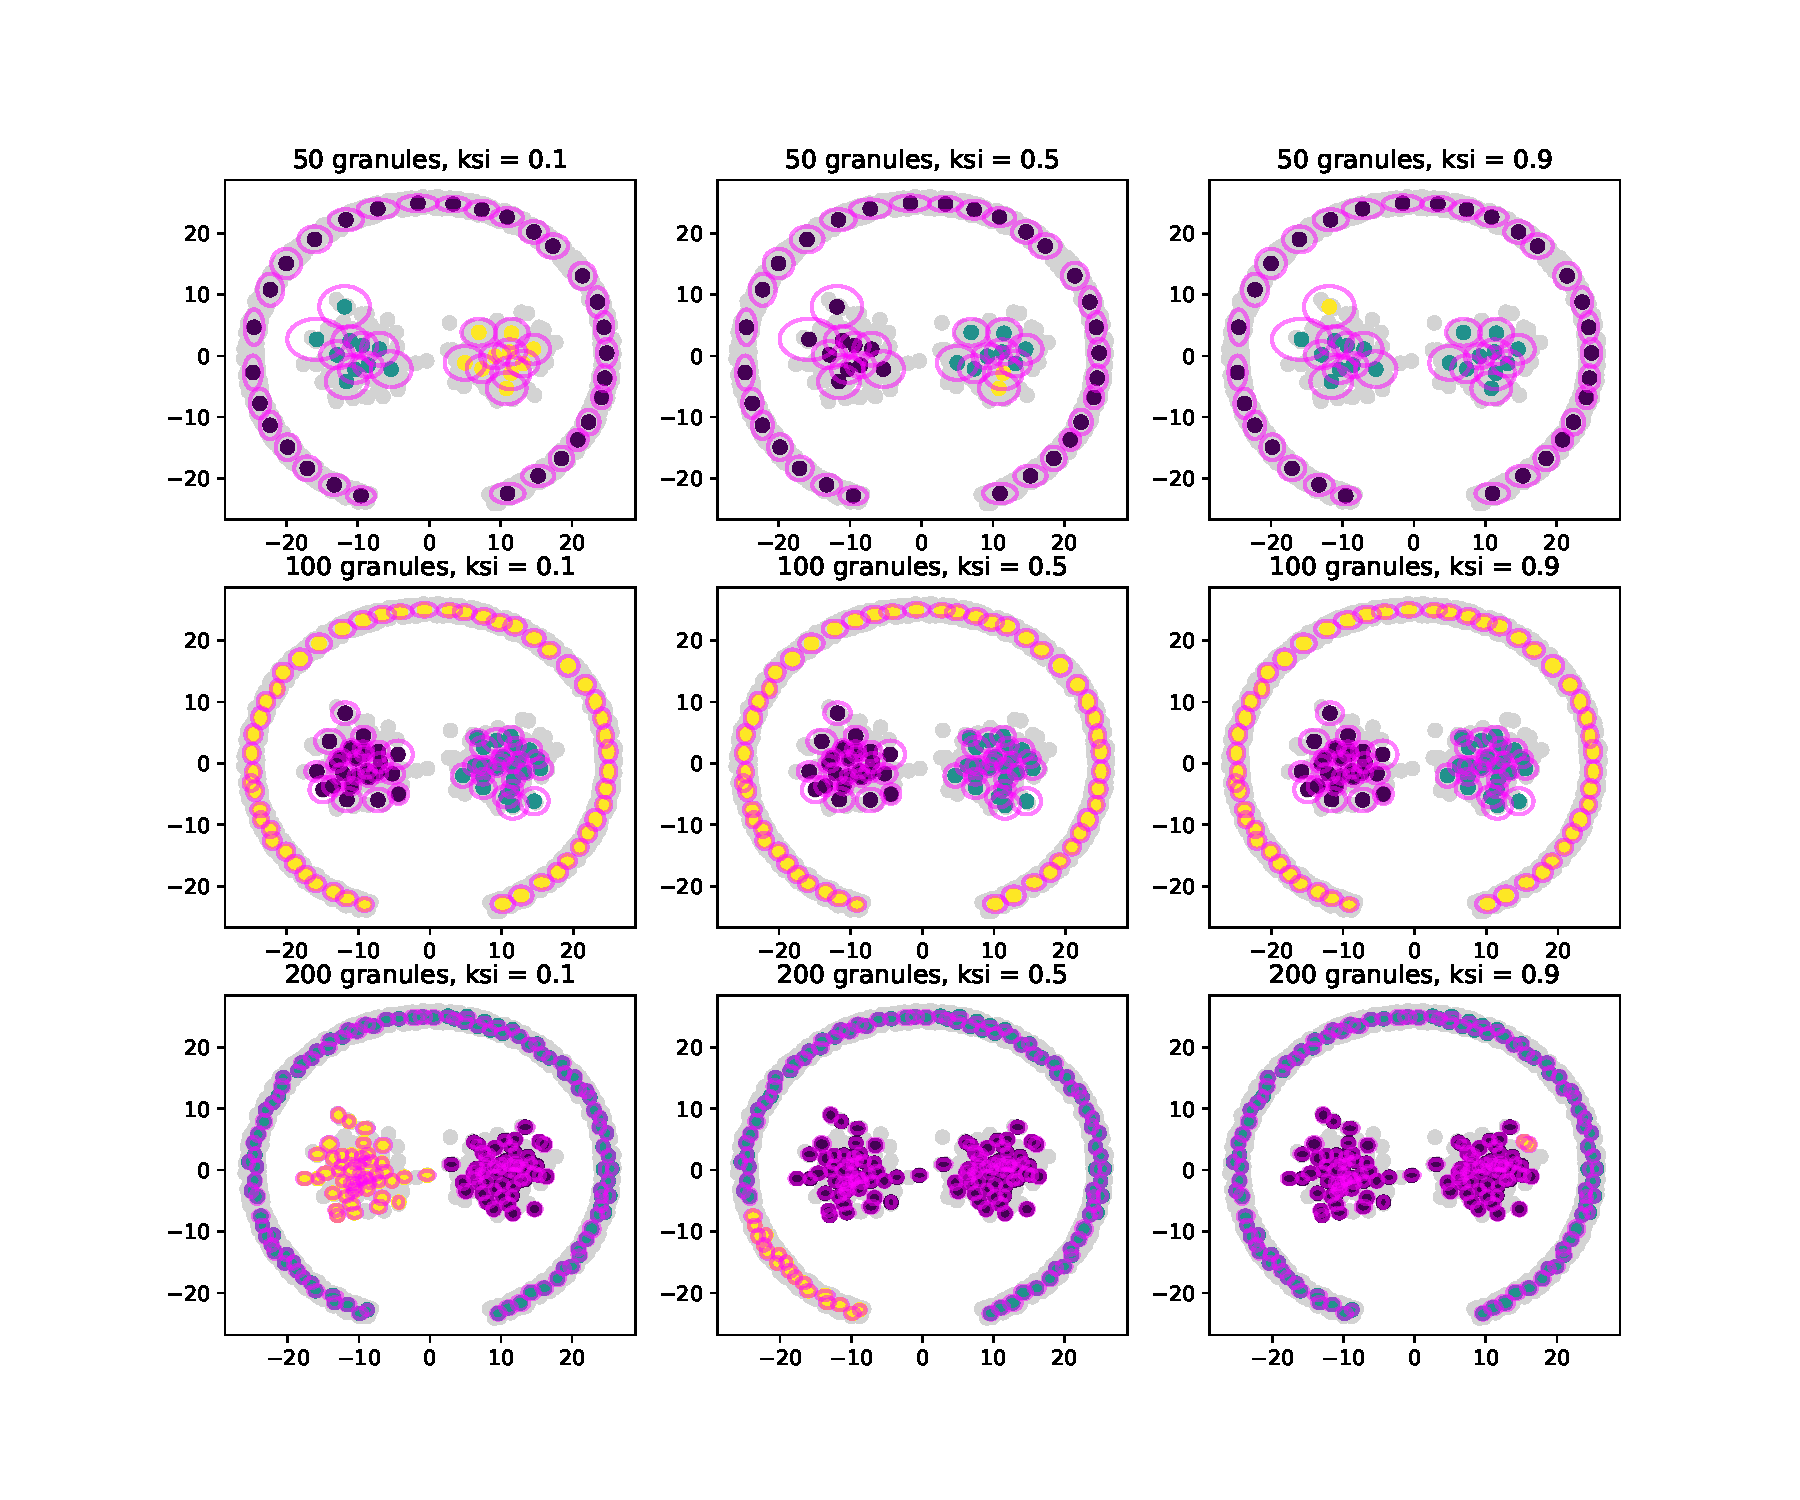
\includegraphics[width=\textwidth]{./laguna2000g.pdf}
\caption{Efekty wykonania grupowania \MojAlg\ dla danych \laguna\  o rozmiarze 2000 i gaussowskiej relacji między liczbami rozmytymi.}
\label{fig:laguna2000g}
\end{figure}

\begin{figure}
\centering
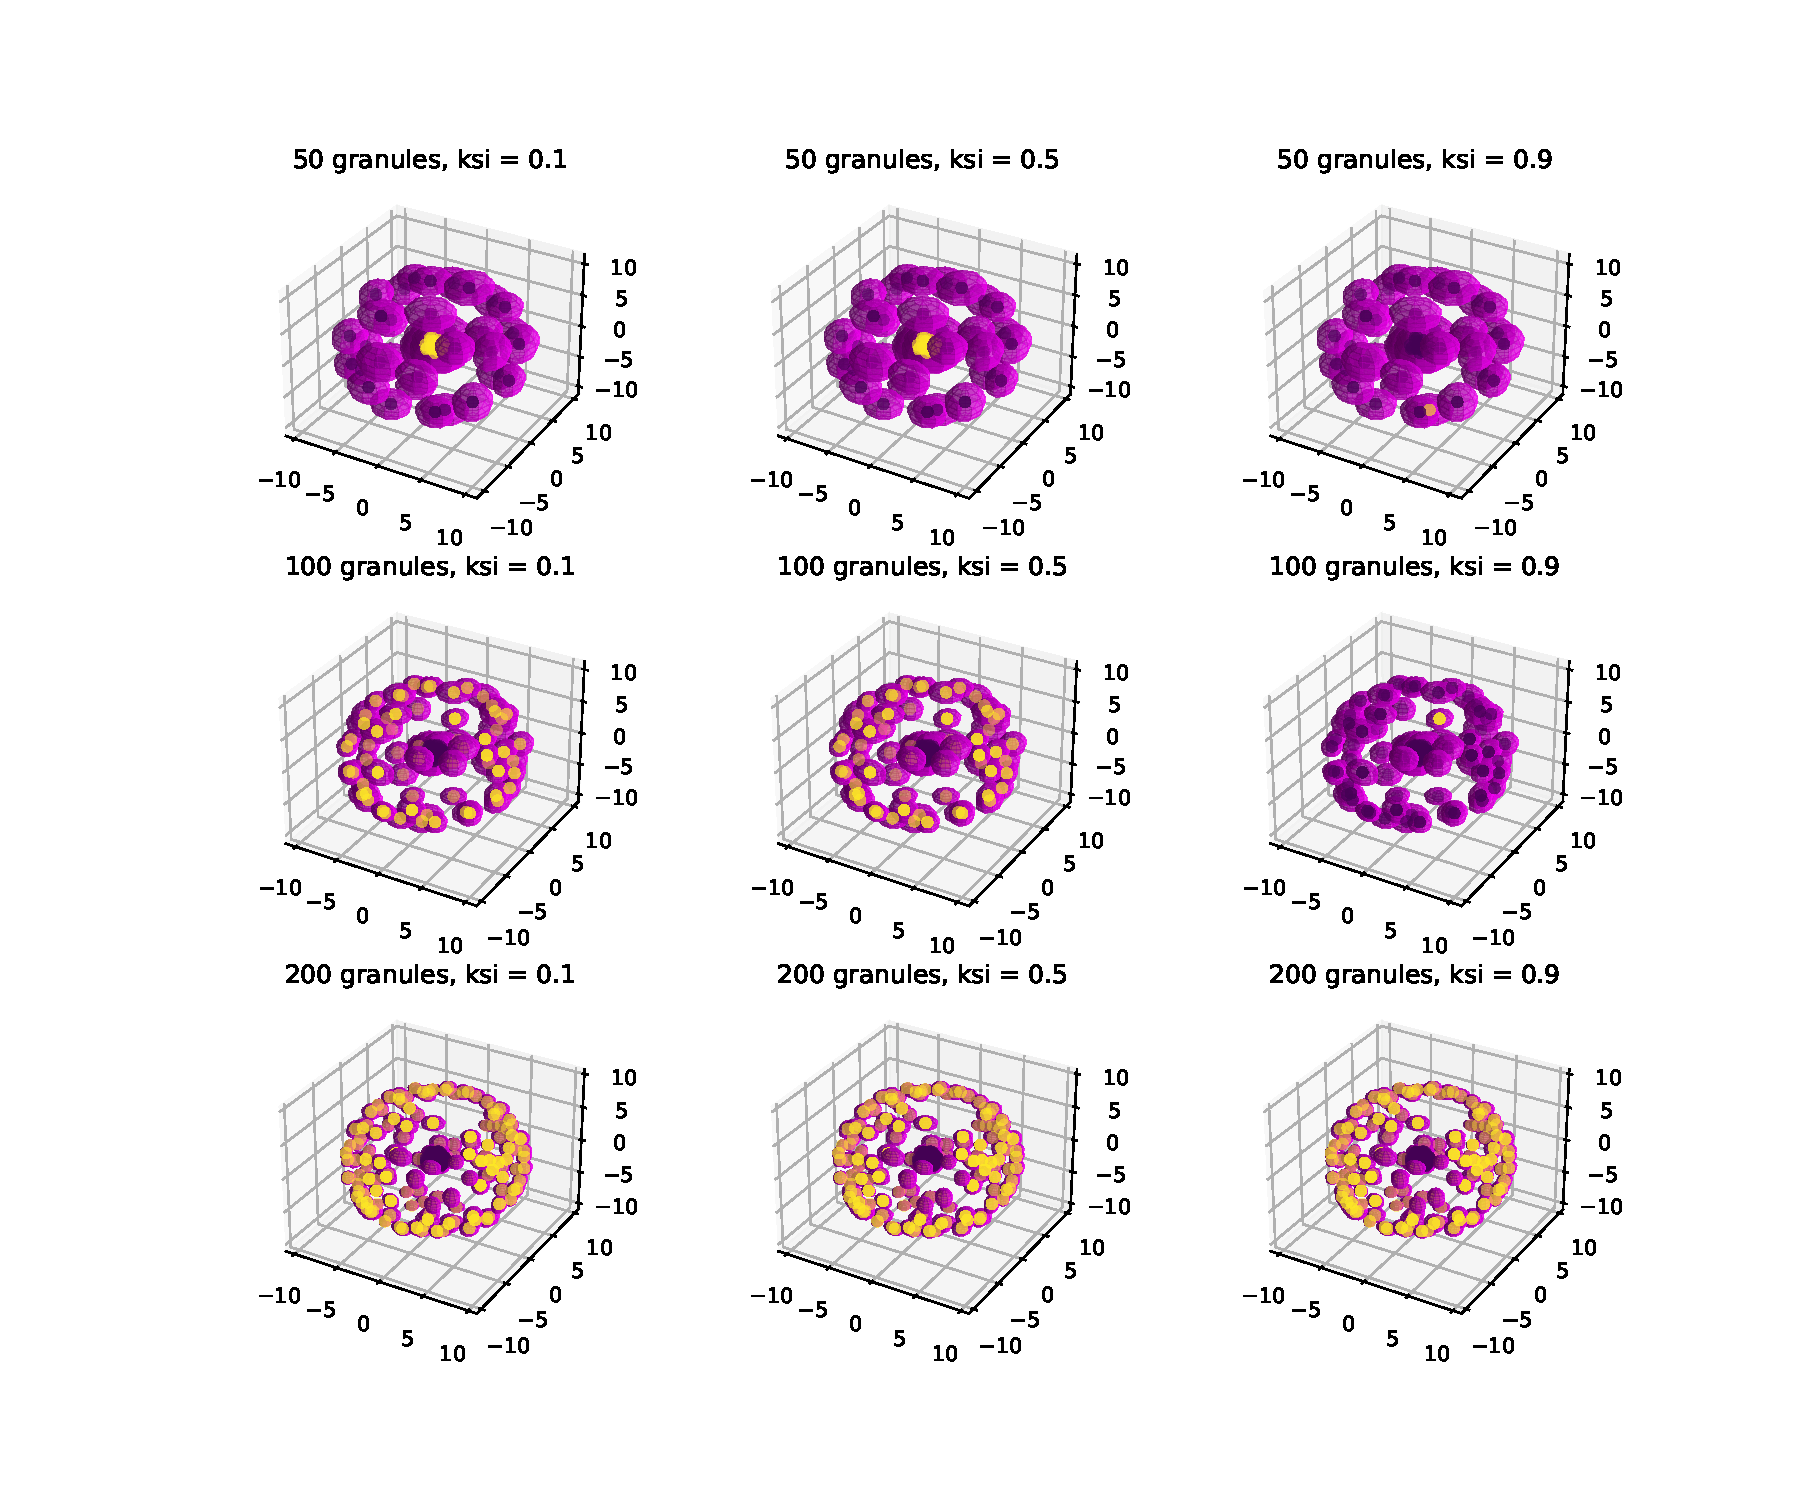
\includegraphics[width=\textwidth]{./spheres1000e.pdf}
\caption{Efekty wykonania grupowania hierarchicznego granul dla danych \spheres\  o rozmiarze 1000 i wykładniczej relacji między liczbami rozmytymi.}
\label{fig:spheres1000e}
\end{figure}

Podobnie jak w przypadku \SingleLinkage{}, najlepsze wyniki dla łączności \CompleteLinkage{} uzyskano dla danych \crescents{}. Inaczej jest w przypadku najgorszych wyników: dane \laguna\ mają najgorszą dokładność i precyzję, a dane \spheres\ -- najgorszą trafność. Wszystkie wyniki są znacznie gorsze od uzyskanych dla \SingleLinkage{}, za wyjątkiem trafności dla danych \blobs{}.


\paragraph{Zależność od liczby granul}

Średnią dokładność, trafność i precyzję grupowania danych w zależności od liczby granul przedstawiono odpowiednio w tabelach \ref{id:tab:acc-gn}, \ref{id:tab:rec-gn} i \ref{id:tab:prec-gn}. W przypadku łączności \SingleLinkage{} najlepsze wyniki osiągane są dla 100 granul, a dla \CompleteLinkage{} -- dla 50.

Dla danych takich, jak \circles{} (rys. \ref{fig:circles20000g}) czy \crescents{} (rys. \ref{fig:crescents1000t}), gdzie klastry mają podobną liczebność i gęstość, zwiększenie liczby granul powoduje ich zagęszczenie, przy równomiernym rozłożeniu.

Inaczej jest w przypadku danych \blobs{} (rys. \ref{fig:blobs1000e}). Dla większych liczebności granul, możliwe jest, że algorytm rozmytych $c$-średnich nie wyznacza ani jednego środka granuli w dwóch mniejszych klastrach, przez co niemożliwe jest poprawne grupowanie.

% TODO tu można zrobić analizę przynależności (niebieskie wykresy)

\begin{table}
\centering
\caption{Dokładność grupowania hierarchicznego danych w zależności od liczby granul i łączności}
\label{id:tab:acc-gn}
\begin{tabular}{rrr}
\toprule
	liczba granul & dokładność \SingleLinkage{} & dokładność \CompleteLinkage{} \\
\midrule
	50 & 97,7201\% & 70,1218\% \\
	100 & 98,8127\% & 68,1147\% \\
	200 & 98,6939\% & 65,7058\% \\
\bottomrule
\end{tabular}
\end{table} 

\begin{table}
\centering
\caption{Trafność grupowania hierarchicznego danych w zależności od liczby granul i łączności}
\label{id:tab:rec-gn}
\begin{tabular}{rrr}
\toprule
	liczba granul & trafność \SingleLinkage{} & trafność \CompleteLinkage{} \\
\midrule
	50 & 95,9457\% & 65,1262\% \\
	100 & 96,6480\% & 63,5260\% \\
	200 & 94,3459\% & 61,8105\% \\
\bottomrule
\end{tabular}
\end{table} 

\begin{table}
\centering
\caption{Precyzja grupowania hierarchicznego danych w zależności od liczby granul i łączności}
\label{id:tab:prec-gn}
\begin{tabular}{rrr}
\toprule
	liczba granul & precyzja \SingleLinkage{} & precyzja \CompleteLinkage{} \\
\midrule
	50 & 95,9749\% & 62,6649\% \\
	100 & 96,4913\% & 59,9919\% \\
	200 & 94,1259\% & 56,8863\% \\
\bottomrule
\end{tabular}
\end{table} 

\paragraph{Zależność od typu relacji}

Średnią dokładność grupowania danych w zależności od typu relacji między granulami dla różnych łączności przedstawiono w tabeli \ref{id:tab:acc-rt}, trafność -- w tabeli \ref{id:tab:rec-rt}, a precyzję -- w tabeli \ref{id:tab:prec-rt}.
Wyniki w zależności od typu relacji są zbliżone, jednak najlepszą dokładność, trafność i precyzję odnotowano dla relacji trójkątnej i łączności \SingleLinkage{}. Wiąże się to ze skończonym nośnikiem liczb rozmytych.
Jako że większość kształtów danych zawiera dysproporcje w liczebności, średnie wartości trafności i precyzji są niższe od odpowiadającym im wartościom dokładności.

\begin{table}
\centering
\caption{Dokładność grupowania hierarchicznego danych w zależności od typu relacji i łączności}
\label{id:tab:acc-rt}
\begin{tabular}{rrr}
\toprule
	typ relacji & dokładność \SingleLinkage{} & dokładność \CompleteLinkage{} \\
\midrule
	trójkątna & 99,4364\% & 67,5915\% \\
	wykładnicza & 97,9782\% & 67,9194\% \\
	gaussowska & 97,8122\% & 68,4314\% \\
\bottomrule
\end{tabular}
\end{table} 
\ksremark{Dokładność w tab. \ref{id:tab:acc-rt} jest układa się dokładnie odwrotnie dla \SingleLinkage\ i dla \CompleteLinkage. Tzn. tam gdzie \SingleLinkage\ jest najlepszy, tam \CompleteLinkage\ jest najgorszy i odwrotnie. Dlaczego tak się dzieje?}

\begin{table}
\centering
\caption{Trafność grupowania hierarchicznego danych w zależności od typu relacji i łączności}
\label{id:tab:rec-rt}
\begin{tabular}{rrr}
\toprule
	typ relacji & trafność \SingleLinkage{} & trafność \CompleteLinkage{} \\
\midrule
	trójkątna & 97,7833\% & 63,6595\% \\
	wykładnicza & 94,1950\% & 63,4156\% \\
	gaussowska & 94,1950\% & 63,4376\% \\
\bottomrule
\end{tabular}
\end{table} 

\begin{table}
\centering
\caption{Precyzja grupowania hierarchicznego danych w zależności od typu relacji i łączności}
\label{id:tab:prec-rt}
\begin{tabular}{rrr}
\toprule
	typ relacji & precyzja \SingleLinkage{} & precyzja \CompleteLinkage{} \\
\midrule
	trójkątna & 97,5440\% & 59,9329\% \\
	wykładnicza & 94,9921\% & 59,8046\% \\
	gaussowska & 94,0560\% & 59,8056\% \\
\bottomrule
\end{tabular}
\end{table} 

\paragraph{Zależność od parametru $\xi$}

Średnią dokładność, trafność i precyzję grupowania danych w zależności od parametru $\xi$ przedstawiono na rys. \ref{fig:xi-acc}.

Dla \SingleLinkage{}, najwyższą dokładność, trafność i precyzję -- odpowiednio 99,6232\%, 98,5214\% i 98,2\% -- osiągnięto dla $\xi=0,05$, wartości metryk spadają wraz ze wzrostem wartości parametru. Powyżej $\xi=0,85$ następuje gwałtowne załamanie na wykresie wyników.

Zależność dokładności jest przeciwna dla \CompleteLinkage{}: najlepsze wyniki -- 69,5779\% -- osiągnięto dla $\xi=0,95$. Trafność i precyzja nie wpisują się w tą zależność -- ich wartości wahają się odpowiednio około 63-64\% i 60\%. Najwyższa wartość trafności wynosi 64,13\% dla $\xi=0,2$, a precyzji -- 60,2063\% dla $\xi=0,85$.
\ksremark{Trzeba skomentować te wyniki.}
\begin{figure}
	\centering
	\begin{subfigure}{0.48\textwidth}
		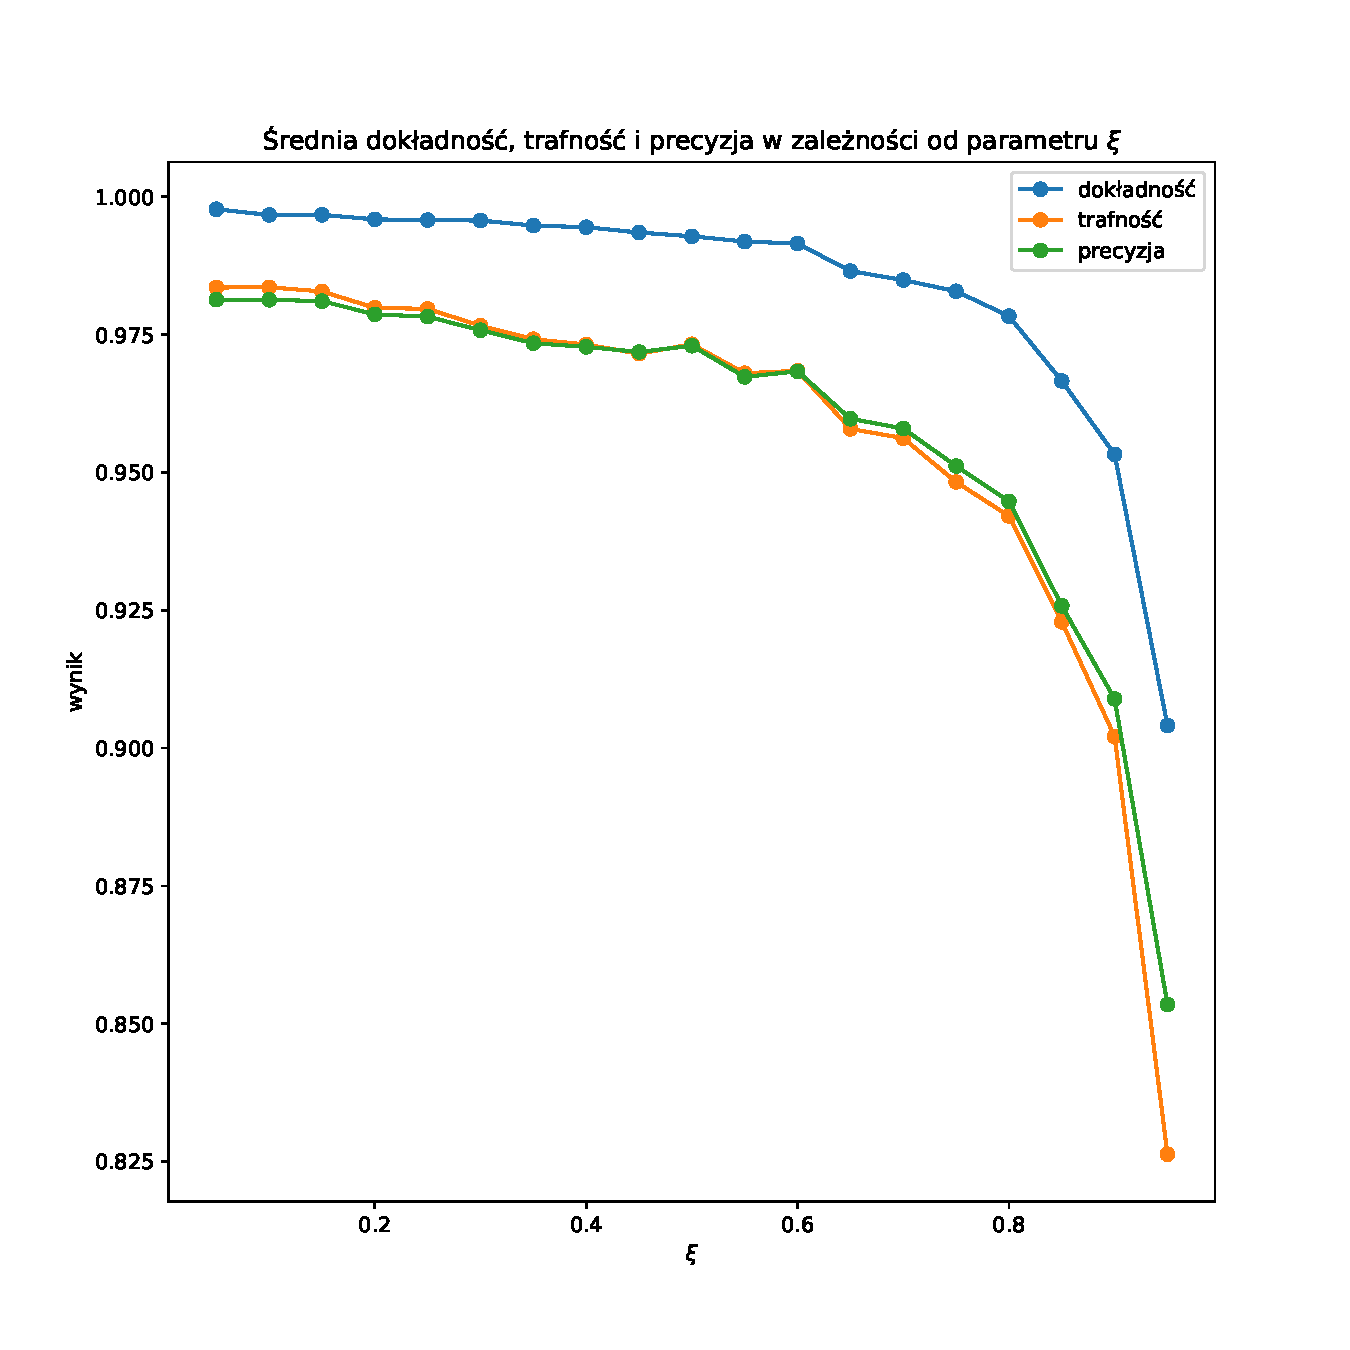
\includegraphics[width=\textwidth]{./xi_acc_sl.pdf}
		\caption{\SingleLinkage}
		\label{fig:xi-acc-sl}
	\end{subfigure}
	\hfill
	\begin{subfigure}{0.48\textwidth}
		
\includegraphics[width=\textwidth]{./xi_acc_cl.pdf}
		\caption{\CompleteLinkage}
	\label{fig:xi-acc-cl}
	\end{subfigure}
	
%	\begin{subfigure}{0.4\textwidth}
%		%    \includegraphics[width=\textwidth]{sciezka}
%		tutaj rysunek
%		\caption{Lewy dolny rysunek.}
%		\label{fig:lewy-dolny}
%	\end{subfigure}
%	\hfill
%	\begin{subfigure}{0.4\textwidth}
%		%    \includegraphics[width=\textwidth]{sciezka}
%		tutaj rysunek
%		\caption{Prawy dolny rysunek.}
%		\label{fig:prawy-dolny}
%	\end{subfigure}
	
	\caption{Zależność dokładności, trafności i precyzji grupowania od wartości parametru $\xi$.}
	\label{fig:xi-acc}
\end{figure}


\subsubsection{Dane Brightkite i Gowalla}

Algorytm grupowania hierarchicznego dostarczony przez bibliotekę scikit-learn nie odnajduje oczekiwanych klastrów (rys. \ref{fig:brightkite-nonfuzzy}).
Przedstawione na rys. \ref{fig:brightkite-fuzzy} wyniki algorytmu rozmytego są bliższe oczekiwaniom, klastry zlokalizowane są we współrzędnych odpowiadającym kontynentom.
Wstępna granulacja FCM pozwoliła na eliminację szumów, na które wrażliwy jest algorytm grupowania hierarchicznego.

\begin{figure}
\centering
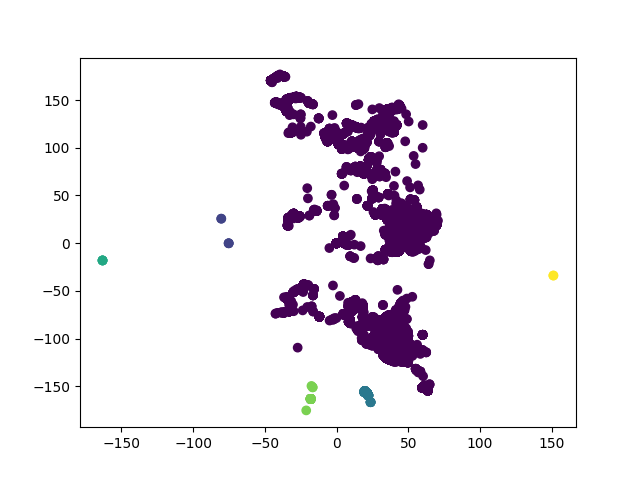
\includegraphics{./brightkite_nonfuzzy.png}
\caption{Dane \brightkite (próbka 100000 współrzędnych) zgrupowane do 6 klastrów algorytmem ostrym (AgglomerativeClustering biblioteki scikit-learn).}
\label{fig:brightkite-nonfuzzy}
\end{figure}

\begin{figure}
\centering
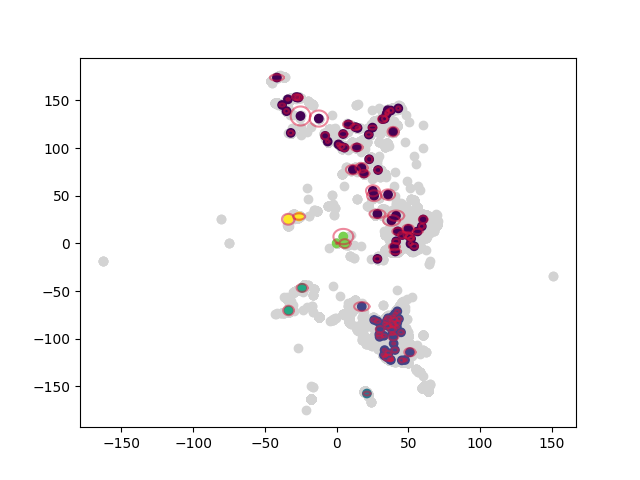
\includegraphics{./brightkite_fuzzy.png}
\caption{Dane \brightkite (próbka 100000 współrzędnych) zgrupowane do 6 klastrów algorytmem \MojAlg{}.}
\label{fig:brightkite-fuzzy}
\end{figure}

%
% 
%
%Rozdział przedstawia przeprowadzone badania. Jest to zasadnicza część i~musi wyraźnie dominować w~pracy.
%Badania i analizę wyników należy przeprowadzić, tak jak jest przyjęte w środowisku naukowym (na przykład korzystanie z danych benchmarkowych, walidacja krzyżowa, zapewnienie powtarzalności testów itd). 
%
%\section{Metodyka badań}
%
%\begin{itemize}
%\item opis metodyki badań
%\item opis stanowiska badawczego (opis interfejsu aplikacji badawczych -- w~załączniku)
%\end{itemize}
%
%
%\section{Zbiory danych}
%
%\begin{itemize}
%\item opis danych
%\end{itemize}
%
%
%\section{Wyniki}
%
%\begin{itemize}
%\item prezentacja wyników, opracowanie i poszerzona dyskusja  wyników, wnioski
%\end{itemize}
%
% 
%\begin{table}
%\centering
%\caption{Opis tabeli nad nią.}
%\label{id:tab:wyniki}
%\begin{tabular}{rrrrrrrr}
%\toprule
%	         &                                     \multicolumn{7}{c}{metoda}                                      \\
%	         \cmidrule{2-8}
%	         &         &         &        \multicolumn{3}{c}{alg. 3}        & \multicolumn{2}{c}{alg. 4, $\gamma = 2$} \\
%	         \cmidrule(r){4-6}\cmidrule(r){7-8}
%	$\zeta$ &     alg. 1 &   alg. 2 & $\alpha= 1.5$ & $\alpha= 2$ & $\alpha= 3$ &   $\beta = 0.1$  &   $\beta = -0.1$ \\
%\midrule
%	       0 &  8.3250 & 1.45305 &       7.5791 &    14.8517 &    20.0028 & 1.16396 &                       1.1365 \\
%	       5 &  0.6111 & 2.27126 &       6.9952 &    13.8560 &    18.6064 & 1.18659 &                       1.1630 \\
%	      10 & 11.6126 & 2.69218 &       6.2520 &    12.5202 &    16.8278 & 1.23180 &                       1.2045 \\
%	      15 &  0.5665 & 2.95046 &       5.7753 &    11.4588 &    15.4837 & 1.25131 &                       1.2614 \\
%	      20 & 15.8728 & 3.07225 &       5.3071 &    10.3935 &    13.8738 & 1.25307 &                       1.2217 \\
%	      25 &  0.9791 & 3.19034 &       5.4575 &     9.9533 &    13.0721 & 1.27104 &                       1.2640 \\
%	      30 &  2.0228 & 3.27474 &       5.7461 &     9.7164 &    12.2637 & 1.33404 &                       1.3209 \\
%	      35 & 13.4210 & 3.36086 &       6.6735 &    10.0442 &    12.0270 & 1.35385 &                       1.3059 \\
%	      40 & 13.2226 & 3.36420 &       7.7248 &    10.4495 &    12.0379 & 1.34919 &                       1.2768 \\
%	      45 & 12.8445 & 3.47436 &       8.5539 &    10.8552 &    12.2773 & 1.42303 &                       1.4362 \\
%	      50 & 12.9245 & 3.58228 &       9.2702 &    11.2183 &    12.3990 & 1.40922 &                       1.3724 \\
%\bottomrule
%\end{tabular}
%\end{table}  
%
%
% 
%\begin{figure}
%\centering
%\begin{tikzpicture}
%\begin{axis}[
%    y tick label style={
%        /pgf/number format/.cd,
%            fixed,   % po zakomentowaniu os rzednych jest indeksowana wykladniczo
%            fixed zerofill, % 1.0 zamiast 1
%            precision=1,
%        /tikz/.cd
%    },
%    x tick label style={
%        /pgf/number format/.cd,
%            fixed,
%            fixed zerofill,
%            precision=2,
%        /tikz/.cd
%    }
%]
%\addplot [domain=0.0:0.1] {rnd};
%\end{axis} 
%\end{tikzpicture}
%\caption{Podpis rysunku po rysunkiem.}
%\label{fig:2}
%\end{figure}
%
%
%\begin{figure}
%\begin{lstlisting}
%if (_nClusters < 1)
%	throw std::string ("unknown number of clusters");
%if (_nIterations < 1 and _epsilon < 0)
%	throw std::string ("You should set a maximal number of iteration or minimal difference -- epsilon.");
%if (_nIterations > 0 and _epsilon > 0)
%	throw std::string ("Both number of iterations and minimal epsilon set -- you should set either number of iterations or minimal epsilon.");
%\end{lstlisting}
%\caption{Przykład pseudokodu}
%\end{figure}


% TODO

\chapter{Podsumowanie}

%\begin{itemize}
%\item Jaki problem rozwiązałæm?
%\item Jak ten problem rozwiązałæm?
%\item Jakie są dobre i słabe strony mojego rozwiązania?
%\item Czy mogę sformułować jakieś rekomendacje?
%\end{itemize}

\begin{itemize}
\item syntetyczny opis wykonanych prac
\item wnioski
\item możliwość rozwoju, kontynuacji prac, potencjalne nowe kierunki
\item Czy cel pracy zrealizowany? 
\end{itemize}



\backmatter

\cleardoublepage
\phantomsection
%\bibliographystyle{plplain}  % bibtex
%\bibliography{biblio} % bibtex
\addcontentsline{toc}{chapter}{Bibliografia}
\printbibliography           % biblatex

\begin{appendices}

% TODO
\chapter{Dokumentacja techniczna}


% TODO
\chapter{Spis skrótów i symboli}

\begin{itemize}
\item[$N$] liczebność zbioru danych
\item[$\mu$] stopnień przyleżności do zbioru
\item[FCM] algorytm fuzzy-c means 
\end{itemize}

% TODO
\chapter{Lista dodatkowych plików, uzupełniających tekst pracy (jeżeli dotyczy)} 

W systemie do pracy dołączono dodatkowe pliki zawierające:
\begin{itemize}
\item źródła programu,
\item zbiory danych użyte w~eksperymentach,
\item film pokazujący działanie opracowanego oprogramowania lub zaprojektowanego i wykonanego urządzenia,
\item itp.
\end{itemize}


\listoffigures
\addcontentsline{toc}{chapter}{Spis rysunków}
\listoftables
\addcontentsline{toc}{chapter}{Spis tabel}

\end{appendices}

\end{document}


%% Finis coronat opus.

